\documentclass{../commun/prepacours}
\usepackage{../commun/raccourcis}

% \setlength{\headheight}{15.5pt}

\annee{2026-2027}
\filiere{MPI / MPI*}
\etablissement{Lycée Champollion}
\auteur{L. Dehmas}

\pgfplotsset{compat=1.18} % Utiliser une version récente pour le z-buffer


\usetikzlibrary{arrows.meta, positioning}
\usepackage{pdflscape}
\graphicspath{{./images/}}

\makeatletter
\gdef\@numchapitre{}
\gdef\@titrechapitre{TD de Mathématiques}
\makeatother

\newcommand{\docType}{TDs}

\begin{document}
\pagestyle{empty}
\newgeometry{
  top=4cm,
  bottom=4cm,
  left=3.5cm,
  right=3.5cm
}

\begin{tikzpicture}[remember picture,overlay]
  \draw[vorange, line width=1.5pt] 
    ([shift={(1.5cm,-1.5cm)}]current page.north west) rectangle 
    ([shift={(-1.5cm,1.5cm)}]current page.south east);
  \draw[vorange!40, line width=0.5pt] 
    ([shift={(1.65cm,-1.65cm)}]current page.north west) rectangle 
    ([shift={(-1.65cm,1.65cm)}]current page.south east);
    
  \node[fill=white, inner xsep=15pt, inner ysep=5pt] 
    at ([yshift=1.5cm]current page.south) {
      \color{black!60}\small\scshape Version du \today
    };
\end{tikzpicture}

\begin{center}
  \makeatletter
  \vspace*{1.5cm}
  
  {\large\color{black!70}\scshape \@etablissement \ -- \ Filière \@filiere \par}
  \vspace{3.5cm}
  
  {\fontsize{40}{48}\selectfont\bfseries\color{vorange!95!black} Maths spé\par}
  \vspace{0.8cm}
  
  \begin{tikzpicture}
    \draw[vorange, line width=1.5pt] (-3.5,0) -- (3.5,0);
    \fill[vorange] (0,0) ++(0,3.5pt) -- ++(3.5pt,-3.5pt) -- ++(-3.5pt,-3.5pt) -- ++(-3.5pt,3.5pt) -- cycle;
  \end{tikzpicture}\par
  \vspace{0.8cm}
  
  {\fontsize{34}{42}\selectfont\bfseries\scshape\color{black} \docType \par}

  \vspace{4.5cm}

  {\Large\bfseries D'après les cours de Yann Quibel\par}
  \vspace{0.6cm}
  {\normalsize\itshape Notes rédigées par L. Dehmas, C. Perry et al.\par}
  \makeatother
\end{center}


\clearpage
\begin{center}
  \vspace*{0.8cm}

  \begin{tikzpicture}[remember picture,overlay]
    \draw[vorange!50, line width=0.6pt] 
      ([shift={(15mm,-15mm)}]current page.north west) -- ++(8mm,0) 
      ([shift={(15mm,-15mm)}]current page.north west) -- ++(0,-8mm);
    \draw[vorange!50, line width=0.6pt] 
      ([shift={(-15mm,-15mm)}]current page.north east) -- ++(-8mm,0) 
      ([shift={(-15mm,-15mm)}]current page.north east) -- ++(0,-8mm);
    \draw[vorange!50, line width=0.6pt] 
      ([shift={(15mm,15mm)}]current page.south west) -- ++(8mm,0) 
      ([shift={(15mm,15mm)}]current page.south west) -- ++(0,8mm);
    \draw[vorange!50, line width=0.6pt] 
      ([shift={(-15mm,15mm)}]current page.south east) -- ++(-8mm,0) 
      ([shift={(-15mm,15mm)}]current page.south east) -- ++(0,8mm);
  \end{tikzpicture}

  {\LARGE\bfseries\scshape Crédits \& Remerciements\par}
  \vspace{0.35cm}
  \begin{tikzpicture}
    \draw[vorange, line width=1pt] (-4,0) -- (-0.4,0);
    \fill[vorange] (0,0) ++(0,2.2pt) -- ++(2.2pt,-2.2pt) -- ++(-2.2pt,-2.2pt) -- ++(-2.2pt,2.2pt) -- cycle;
    \fill[vorange!60] (-0.7,0) circle (0.9pt) (0.7,0) circle (0.9pt);
    \draw[vorange, line width=1pt] (0.4,0) -- (4,0);
  \end{tikzpicture}\par

  \vspace{1.1cm}

  \begin{minipage}{0.85\textwidth}
    \centering
    \begin{tikzpicture}
      \draw[vorange, line width=0.8pt] (0,0) -- (0.44\linewidth,0);
      \draw[vorange, line width=0.6pt] (0.47\linewidth,0) circle (2pt);
      \fill[vorange] (0.5\linewidth,0) ++(0,2.2pt) -- ++(2.2pt,-2.2pt) -- ++(-2.2pt,-2.2pt) -- ++(-2.2pt,2.2pt) -- cycle;
      \draw[vorange, line width=0.6pt] (0.53\linewidth,0) circle (2pt);
      \draw[vorange, line width=0.8pt] (0.56\linewidth,0) -- (\linewidth,0);
    \end{tikzpicture}\par
    \vspace{0.6cm}

    {\large\bfseries\color{vorange!95!black}\scshape Auteurs principaux\par}
    \vspace{0.45em}
    \begin{tabular*}{\linewidth}{@{\extracolsep{\fill}}cc@{}}
      \begin{minipage}[t]{0.45\linewidth}
        \raggedleft
        {\Large\bfseries L. Dehmas}\\[0.2em]
        {\footnotesize\scshape MPI* 2025--2026}
      \end{minipage}
      &
      \begin{minipage}[t]{0.45\linewidth}
        {\Large\bfseries C. Perry}\\[0.2em]
        {\footnotesize\scshape MPI* 2026--2027}
      \end{minipage}
    \end{tabular*}
    \\[0.5em]
    {\small\itshape Rédaction du cours et des exercices, mise en forme\par}

    \vspace{0.75cm}

    \makeatletter%
    {\large\bfseries\color{vorange!95!black}\scshape Enseignement \& Cours d'origine\par}
    \vspace{0.3em}
    {\Large\bfseries Yann Quibel\par}
    \vspace{0.2em}
    {\small Professeur de mathématiques en \@filiere{} au \@etablissement\par}
    \vspace{0.3em}
    {\small\itshape Ce polycopié reprend et met en forme l'ensemble des cours magistraux\\%
    et travaux dirigés dispensés au cours des années scolaires 2025--2026 et \@annee.\par}
    \makeatother%
    
    \vspace{0.75cm}

    {\large\bfseries\color{vorange!95!black}\scshape Autres contributions\par}
    \vspace{0.5em}

    \newcommand{\csep}{\hspace{0.5em}\tikz[baseline=-0.6ex]{\fill[vorange!80] (0,0) ++(0,1.5pt) -- ++(1.5pt,-1.5pt) -- ++(-1.5pt,-1.5pt) -- ++(-1.5pt,1.5pt) -- cycle;}\hspace{0.5em}}

    \begin{minipage}{0.96\linewidth}
      \centering\normalsize
      \mbox{\textbf{C. Bras} {\footnotesize(\textsc{MPI 2025--2026})}} \csep
      \mbox{\textbf{T. Olinger} {\footnotesize(\textsc{MPI* 2025--2027})}} 
      
      \vspace{0.25em}
      \mbox{\textbf{F. Cerisier} {\footnotesize(\textsc{MPI* 2026--2027})}} \csep
      \mbox{\textbf{E. Meyer Guenego} {\footnotesize(\textsc{MP2I 2026--2027})}}
      
      \vspace{0.25em}
      \mbox{\textbf{E. Allamand} {\footnotesize(\textsc{MPI* 2026--2027})}}
    \end{minipage}
    \\[0.5em]
    {\small\itshape Solutions d'exercices, relectures\par}

    \vspace{0.6cm}
    
    \begin{tikzpicture}
      \draw[vorange, line width=0.8pt] (0,0) -- (0.44\linewidth,0);
      \draw[vorange, line width=0.6pt] (0.47\linewidth,0) circle (2pt);
      \fill[vorange] (0.5\linewidth,0) ++(0,2.2pt) -- ++(2.2pt,-2.2pt) -- ++(-2.2pt,-2.2pt) -- ++(-2.2pt,2.2pt) -- cycle;
      \draw[vorange, line width=0.6pt] (0.53\linewidth,0) circle (2pt);
      \draw[vorange, line width=0.8pt] (0.56\linewidth,0) -- (\linewidth,0);
    \end{tikzpicture}\par
  \end{minipage}

  \vfill

  \makeatletter%
  {\small\scshape \@filiere{} -- \@etablissement\par}
  \vspace{0.25cm}
  {\footnotesize Document composé sous \LaTeX{} -- Année \@annee\par}
  \vspace{0.6cm}
  \makeatother%
\end{center}

\clearpage
\cleardoublepage
\vspace*{3cm}

\begin{center}
  {\LARGE\bfseries\color{vorange!95!black}\scshape Avant-propos\par}
  \vspace{0.4cm}
  \begin{tikzpicture}
    \draw[vorange!50, line width=1pt] (-2,0) -- (2,0);
    \fill[vorange] (0,0) ++(0,2pt) -- ++(2pt,-2pt) -- ++(-2pt,-2pt) -- ++(-2pt,2pt) -- cycle;
  \end{tikzpicture}
\end{center}

\vspace{1.5cm}

\begin{center}
\begin{minipage}{0.85\textwidth}
  \setlength{\parindent}{1.5em}
  \setlength{\parskip}{0.8em}
  \large 

  {\hyphenpenalty=10000\exhyphenpenalty=10000
  Ce polycopié rassemble l'ensemble du cours de notre grand Quibel, ainsi que les travaux dirigés et certaines de leurs corrections.
  
  Il s'agit d'un travail collaboratif. Si vous souhaitez vous porter volontaire pour rédiger des corrections d'exercices ou étoffer certaines sections, faites-vous plaisir : elles seront intégrées au document.
  
  La saisie d'un tel volume de mathématiques étant sujette aux coquilles, si vous voyez une erreur, merci de nous le signaler !

  À cet effet, vous pouvez contribuer au projet sur cette repo : \url{https://github.com/mp2i-mpi-champo/mpi-maths/}.
  \par}
  \vspace{1.8cm}
  \begin{center}
    \itshape Enjoy !
  \end{center}
\end{minipage}
\end{center}

\vfill

\clearpage

\begin{center}
  {\Huge \bfseries Table des matières \par}
  \vspace{1cm}
\end{center}
\tableofcontents
\clearpage
\pagestyle{scrheadings}

\restaurergeometrie

\pagevide

\chapitreintegral{1}{Normes et distances}
\passerenmodeexos
\section{Énoncés des Exercices}

% --- Exercice 1 (Source: Exercice 89 algèbre) ---
\begin{exercice}[Exercice 89 Algèbre]
    Soit $n \in \N$ tel que $n \geqslant 2$. On pose $z = e^{i\frac{2\pi}{n}}$.
    \begin{enumerate}
        \item On suppose $k \in \{1, \dots, n-1\}$. Déterminer le module et un argument du complexe $z^k - 1$.
        \item On pose $S = \sum_{k=0}^{n-1} |z^k - 1|$. Montrer que $S = \frac{2}{\tan \frac{\pi}{2n}}$.
    \end{enumerate}
\end{exercice}

% --- Exercice 2 (Source: Exercice 1 Normes et distances) ---
\begin{exercice}
    Montrer que sur $E = \R^2$, l'application $N$ définie par :
    $$ N(x,y) = \sup \{ |tx+y|, \ t \in [0,1] \} $$
    est une norme et que pour tout $(x,y)$, $N(x,y) = \max(|y|, |x+y|)$.
\end{exercice}

% --- Exercice 3 (Source: Exercice 37 analyse) ---
\begin{exercice}[Exercice 37 Analyse]
    On note $E$ l'espace vectoriel des applications continues de $[0,1]$ dans $\R$.
    On pose, pour $f \in E$ :
    $$ N_\infty(f) = \sup_{x \in [0,1]} |f(x)| \quad \text{et} \quad N_1(f) = \int_0^1 |f(x)| \dx $$
    \begin{enumerate}
        \item 
        \begin{enumerate}
            \item Démontrer que $N_\infty$ et $N_1$ sont deux normes sur $E$.
            \item Démontrer qu'il existe $k > 0$ tel que, pour tout $f$ de $E$, $N_1(f) \leqslant k N_\infty(f)$.
            \item Démontrer que tout ouvert pour la norme $N_1$ est un ouvert pour la norme $N_\infty$.
        \end{enumerate}
        \item Démontrer que les normes $N_1$ et $N_\infty$ ne sont pas équivalentes.
    \end{enumerate}
\end{exercice}

% --- Exercice 4 (Source: Exercice 2) ---
\begin{exercice}
    Soit $E = \{ f \in \mathscr C^1([0,1], \R) \mid f(0)=0 \}$.
    \begin{enumerate}
        \item Justifier pourquoi $E$ est un $\R$-espace vectoriel.
        \item Pour $f \in E$, on définit :
            $$ n(f) = \|f+f'\|_\infty \quad \text{et} \quad N(f) = \|f\|_\infty + \|f'\|_\infty $$
            Montrer que $n$ et $N$ sont deux normes sur $E$.
        \item Montrer qu'elles sont équivalentes.
    \end{enumerate}
\end{exercice}

% --- Exercice 5 (Source: Exercice 3) ---
\begin{exercice}
    On se place dans $E = \mathscr C^p([0,1], \R)$ et on définit pour tout entier $k$ inférieur à $p$, et toute $f \in E$ :
    $$ N_k(f) = \sum_{i=0}^{k-1} |f^{(i)}(0)| + \sup \{ |f^{(k)}(t)|, \ t \in [0,1] \} $$
    \begin{enumerate}
        \item Montrer que $N_k$ est une norme.
        \item Montrer que ces normes sont deux à deux non-équivalentes.
    \end{enumerate}
\end{exercice}

% --- Exercice 6 (Source: Exercice 4) ---
\begin{exercice}
    Soit $E$ l'espace vectoriel des fonctions lipschitziennes de $[0,1]$ dans $\R$. Pour $f \in E$, on pose :
    $$ N(f) = \sup \{ |f(x)|, x \in [0,1] \} + \sup \left\{ \left| \frac{f(x)-f(y)}{x-y} \right|, x \ne y \right\} $$
    Montrer que $N$ est une norme. Est-elle équivalente à la norme infinie ?
\end{exercice}

% --- Exercice 7 (Source: Exercice 5) ---
\begin{exercice}
    On note $E = \{ f \in \mathscr C^2([0,1], \R) \mid f(0)=f(1)=0 \}$ que l'on munit de $\|\cdot\|_\infty$ et de $N$ définie par :
    $$ N(f) = \sqrt{\int_0^1 f''(t)^2 \dt} $$
    \begin{enumerate}
        \item Vérifier que $N$ est une norme sur $E$.
        \item Montrer que pour $f \in E$, $\|f\|_\infty \leqslant N(f)$.
            \textit{Indication : On montrera successivement que pour tout $x$ on a :}
            $$ f(x) \leqslant \sqrt{\int_0^1 f'(t)^2 \dt}, \quad \text{puis} \quad f(x) \leqslant \sqrt{\int_0^1 -f(t)f''(t) \dt} $$
            $$ \text{puis} \quad f(x) \leqslant \sqrt{\|f\|_\infty \sqrt{\int_0^1 f''(t)^2 \dt}} $$
        \item Montrer que $N$ et $\|\cdot\|_\infty$ ne sont pas équivalentes.
    \end{enumerate}
\end{exercice}

% --- Exercice 8 (Source: Exercice 38 analyse) ---
\begin{exercice}[Exercice 38 Analyse]
    On note $\R[X]$ l'espace vectoriel des polynômes à coefficients réels.
    On pose : $\forall P \in E$, $N_1(P) = \sum_{i=0}^n |a_i|$ et $N_\infty(P) = \max_{0 \leqslant i \leqslant n} |a_i|$ 
    où $P = \sum_{i=0}^n a_i X^i$ avec $n \geqslant \deg P$.
    \begin{enumerate}
        \item 
        \begin{enumerate}
            \item Démontrer que $N_\infty$ est une norme sur $\R[X]$.
            \item Dans la suite de l'exercice, on admet que $N_1$ est une norme sur $\R[X]$. 
                Démontrer que tout ouvert pour la norme $N_\infty$ est un ouvert pour la norme $N_1$.
            \item Démontrer que les normes $N_1$ et $N_\infty$ ne sont pas équivalentes.
        \end{enumerate}
        \item On note $\R_k[X]$ le sous-espace vectoriel de $\R[X]$ constitué par les polynômes de degré inférieur ou égal à $k$. 
            On note $N'_1$ la restriction de $N_1$ à $\R_k[X]$ et $N'_\infty$ la restriction de $N_\infty$ à $\R_k[X]$.
            Les normes $N'_1$ et $N'_\infty$ sont-elles équivalentes ?
    \end{enumerate}
\end{exercice}

% --- Exercice 9 (Source: Exercice 6) ---
\begin{exercice}
    On a vu plus haut que dans $E = \R^2$, l'application $N : (x,y) \mapsto \sup \{ |tx+y|, t \in [0,1] \}$ 
    est une norme et que pour tout $(x,y)$, $N(x,y) = \max(|y|, |x+y|)$. Dessiner la boule fermée de centre 0 et de rayon 1.
\end{exercice}

% --- Exercice 10 (Source: Exercice 7) ---
\begin{exercice}
    Soit $B$ une partie d'un espace vectoriel normé $E$ telle qu'il existe $a$ et $R > 0$ tels que $B = B(a,R)$. 
    Montrer que $R$ et $a$ sont uniques.
\end{exercice}

\newpage
\section{Corrections}

% --- Correction 1 ---
\begin{correction}{1}
\begin{enumerate}
    \item On pose $Z = z^k - 1$.
    $$ Z = e^{i\frac{k\pi}{n}} - 1 = e^{i\frac{k\pi}{n}} \left( e^{i\frac{k\pi}{n}} - e^{-i\frac{k\pi}{n}} \right) e^{-i \dots \text{(factorisation par l'arc moitié)}} $$
    Plus précisément :
    $$ z^k - 1 = e^{i\frac{2k\pi}{n}} - 1 = e^{i\frac{k\pi}{n}} \left( e^{i\frac{k\pi}{n}} - e^{-i\frac{k\pi}{n}} \right) = e^{i\frac{k\pi}{n}} \cdot 2i \sin\left(\frac{k\pi}{n}\right) $$
    C'est-à-dire $Z = 2 \sin\left(\frac{k\pi}{n}\right) e^{i\left(\frac{k\pi}{n} + \frac{\pi}{2}\right)}$.

    Pour $k \in \{1, \dots, n-1\}$, on a $0 < \frac{k\pi}{n} < \pi$, donc $\sin\left(\frac{k\pi}{n}\right) > 0$.

    Donc le module de $z^k-1$ est $2\sin\left(\frac{k\pi}{n}\right)$ et un argument est $\frac{k\pi}{n} + \frac{\pi}{2}$.
    \\

    \item On remarque que pour $k=0$, $|z^k-1| = 0$ et $\sin\left(\frac{k\pi}{n}\right) = 0$.
    
    Donc d'après la question précédente, on a $S = 2 \sum_{k=0}^{n-1} \sin\left(\frac{k\pi}{n}\right)$.

    $S$ est donc la partie imaginaire de $T = 2 \sum_{k=0}^{n-1} e^{i\frac{k\pi}{n}}$.

    Comme $e^{i\frac{\pi}{n}} \ne 1$, on a :
    $$ T = 2 \frac{1 - e^{i\pi}}{1 - e^{i\frac{\pi}{n}}} = \frac{4}{1 - e^{i\frac{\pi}{n}}} $$
    Or $1 - e^{i\frac{\pi}{n}} = e^{i\frac{\pi}{2n}} (e^{-i\frac{\pi}{2n}} - e^{i\frac{\pi}{2n}}) = -2i e^{i\frac{\pi}{2n}} \sin\left(\frac{\pi}{2n}\right)$.

    On en déduit que $T = \frac{4}{-2i \sin\left(\frac{\pi}{2n}\right) e^{i\frac{\pi}{2n}}} = \frac{2i}{\sin\left(\frac{\pi}{2n}\right)} e^{-i\frac{\pi}{2n}}$.

    En isolant la partie imaginaire de $T$, et comme $\cos\left(\frac{\pi}{2n}\right) \ne 0$ (car $n \ge 2$), on en déduit que :
    $$ S = \text{Im}(T) = \frac{2}{\sin \frac{\pi}{2n}} \cos \frac{\pi}{2n} = \frac{2}{\tan \frac{\pi}{2n}} $$
\end{enumerate}
\end{correction}

% --- Correction 2 ---
\begin{correction}{2}

    Le plus simple est de commencer par montrer la formule proposée pour $N$.

    À $(x,y)$ fixé, $t \mapsto tx+y$ est affine donc atteint son maximum et son minimum en 0 et 1 sur le segment $[0,1]$.

    Donc la borne supérieure recherchée, qui est la valeur maximale de la valeur absolue
    (car on a affaire à une fonction continue sur un segment), est atteinte soit en 0 soit en 1.

    Ainsi, $N(x,y) = \max(|y|, |x+y|)$. \\

    $N$ est donc bien à valeurs dans $\R^+$. \\

    Soient $x,y, x', y'$ des réels et $\lambda \in \R$.

    \textbf{Séparation :}
    \begin{quote}
        Si $N(x,y) = 0$, \\
        alors $\max(|y|, |x+y|) = 0$, \\
        donc $y = 0$ et $x+y = 0$, \\
        donc $x=0$. \\
        D'où $(x,y) = (0,0)$.
    \end{quote}

    \textbf{Homogénéité :}
    $$ N(\lambda x, \lambda y) = \sup_{t \in [0,1]} |t\lambda x + \lambda y| = |\lambda| \sup_{t \in [0,1]} |tx+y| = |\lambda| N(x,y) $$

    \textbf{Inégalité triangulaire :}
    $$ N((x,y) + (x',y')) = N(x+x', y+y') = \max(|x+x'+y+y'|, |y+y'|) $$
    Or $|x+x'+y+y'| \le |x+y| + |x'+y'| \le N(x,y) + N(x',y')$.

    Et $|y+y'| \le |y| + |y'| \le N(x,y) + N(x',y')$.

    Le maximum de deux nombres inférieurs à $S$ est inférieur à $S$,
    
    donc $N((x,y)+(x',y')) \le N(x,y) + N(x',y')$.
\end{correction}

% --- Correction 3 ---
\begin{correction}{3}
\begin{enumerate}
    \item 
    \begin{enumerate}
        \item
        
        \textbf{$N_\infty$ est une norme :}
        Soit $f \in E$. $f$ est continue sur le segment $[0,1]$,
        donc bornée, $N_\infty(f)$ existe.
        \begin{itemize}
            \item \textit{Séparation :} Si $N_\infty(f) = 0$, alors $\forall t \in [0,1], |f(t)| = 0$, donc $f=0$.
            \item \textit{Homogénéité :} $N_\infty(\lambda f) = \sup |\lambda f(x)| = |\lambda| N_\infty(f)$.
            \item \textit{Inégalité triangulaire :} $|(f+g)(t)| \le |f(t)| + |g(t)| \le N_\infty(f) + N_\infty(g)$,
                donc en passant au sup, $N_\infty(f+g) \le N_\infty(f) + N_\infty(g)$.
        \end{itemize}

        \textbf{$N_1$ est une norme :}
        \begin{itemize}
            \item \textit{Séparation :} Si $N_1(f) = 0$, alors $\int_0^1 |f(t)| \dt = 0$. Or $|f|$ est continue et positive, donc $|f|=0$, soit $f=0$.
            \item \textit{Homogénéité :} Par linéarité de l'intégrale, $N_1(\lambda f) = |\lambda| N_1(f)$.
            \item \textit{Inégalité triangulaire :} $|f(t)+g(t)| \le |f(t)| + |g(t)|$. Par croissance de l'intégrale, $N_1(f+g) \le N_1(f) + N_1(g)$.
        \end{itemize}

        \item $k=1$ convient car $\forall f \in E$, $N_1(f) = \int_0^1 |f(t)| \dt \le \int_0^1 N_\infty(f) \dt = N_\infty(f)$.

        \item L'application identité de $(E, N_\infty)$ vers $(E, N_1)$ est continue car linéaire et vérifiant $N_1(f) \le k N_\infty(f)$.
        L'image réciproque d'un ouvert par une application continue étant un ouvert, on en déduit qu'un ouvert pour la norme $N_1$ est un ouvert pour la norme $N_\infty$.     
    \end{enumerate}

    \item
    Pour $f_n(t) = t^n$, on a $N_1(f_n) = \frac{1}{n+1}$ et $N_\infty(f_n) = 1$.
    Donc $\lim_{n \to +\infty} \frac{N_\infty(f_n)}{N_1(f_n)} = +\infty$. Les normes ne sont pas équivalentes.
\end{enumerate}
\end{correction}

% --- Correction 4 ---
\begin{correction}{4}
\begin{enumerate}
    \item $E$ est un sous-ensemble non vide de $C^1([0,1], \R)$ (contient la fonction nulle). 
    
    Il est stable par combinaison linéaire, c'est donc un sous-espace vectoriel.

    \item $n$ et $N$ sont à valeurs dans $\R^+$. Soient $f,g \in E, \lambda \in \R$.

    \textit{Pour $n(f)$ :}
    \begin{itemize}
        \item \textbf{Séparation :} Si $n(f)=0$,
        \begin{quote}
            alors $\|f+f'\|_\infty = 0$, donc $f+f'=0$. \\
            C'est une équation différentielle $y' + y = 0$. \\
            Il existe $\alpha$ tel que $f(x) = \alpha e^{-x}$. \\
            Or $f(0)=0$, donc $\alpha=0$ et $f=0$.
        \end{quote}
        \item \textbf{Homogénéité :} $n(\lambda f) = \|\lambda(f+f')\|_\infty = |\lambda| n(f)$.
        \item \textbf{Inégalité triangulaire :} $n(f+g) = \|(f+g) + (f+g)'\|_\infty \le \|f+f'\|_\infty + \|g+g'\|_\infty = n(f) + n(g)$.
    \end{itemize}

    \textit{Pour $N(f)$ :}
    Si $N(f)=0$, alors $\|f\|_\infty = 0$ et $\|f'\|_\infty = 0$, donc $f=0$. 
    
    L'homogénéité et l'inégalité triangulaire découlent directement des propriétés de la norme $\|\cdot\|_\infty$.

    \item Il est clair par inégalité triangulaire que pour tout $f \in E$, $n(f) \le \|f\|_\infty + \|f'\|_\infty = N(f)$.

    Pour l'autre sens, majorons $\|f\|_\infty$ par $n(f)$.
    
    Soit $x \in [0,1]$. Posons $g(x) = e^x f(x)$. 
    \begin{quote}
        On a $f(x) = e^{-x} g(x) = e^{-x} (g(x)-g(0)) = e^{-x} \int_0^x g'(t) \dt$. \\
        Or $g'(t) = e^t (f(t)+f'(t))$. \\
        Donc $|f(x)| \le e^{-x} \int_0^x e^t |f(t)+f'(t)| \dt \le 1 \cdot \int_0^1 e^1 n(f) \dt = e \cdot n(f)$. \\
        Ceci étant vrai pour tout $x$, $\|f\|_\infty \le e \cdot n(f)$. \\
        Alors $\|f'\|_\infty = \|(f+f') - f\|_\infty \le n(f) + \|f\|_\infty \le (1+e)n(f)$. \\
        Au total, $N(f) = \|f\|_\infty + \|f'\|_\infty \le (1+2e) n(f)$. 
    \end{quote}
    Les normes sont équivalentes.
\end{enumerate}
\end{correction}

% --- Correction 5 ---
\begin{correction}{5}
\begin{enumerate}
    \item  $N_k(f)$ est bien définie car $f^{(k)}$ est continue sur un segment donc bornée.
        \begin{itemize}
            \item \textbf{Séparation :} Si $N_k(f) = 0$, 
            \begin{quote}
                alors $\|f^{(k)}\|_\infty = 0$ donc $f^{(k)} = 0$. \\
                $f$ est un polynôme de degré $\le k-1$. \\
                De plus, $f^{(i)}(0) = 0$ pour $i < k$. \\
                La formule de Taylor en 0 montre que $f=0$.
            \end{quote}
            \item \textbf{Homogénéité :} Immédiate par linéarité de la dérivation.
            \item \textbf{Inégalité triangulaire :} Immédiate par inégalité triangulaire dans $\R$ et pour la norme infinie.
        \end{itemize}

    \item Considérons la suite $f_n(x) = x^n$.
    
    Soient $k_1 < k_2$. Pour $n > k_2$, on a $N_{k_1}(f_n) \approx \frac{n!}{(n-k_1)!}$ (termes dominant en norme infinie sur $[0,1]$).

    Le rapport $\frac{N_{k_1}(f_n)}{N_{k_2}(f_n)}$ tend vers 0 quand $n$ tend vers l'infini 
    
    \begin{quote}
        (le degré de dérivation $k_2$ "tue" moins de termes $n$ que $k_1$ ? \\
        Non, c'est l'inverse. $f^{(k)}(x) = n(n-1)\dots(n-k+1)x^{n-k}$. $\|f^{(k)}\|_\infty \approx n^k$. \\
        Donc $N_{k_1} \approx n^{k_1}$ et $N_{k_2} \approx n^{k_2}$. Le rapport tend vers 0).
    \end{quote}

    Conclusion : les normes ne sont pas équivalentes.
\end{enumerate}
\end{correction}

% --- Correction 6 ---
\begin{correction}{6}

Notons $\Delta = \{(x,x), x \in [0,1]\}$ et $A = [0,1]^2 \setminus \Delta$.

Puisque $f$ est lipschitzienne, le taux d'accroissement $g_f(x,y) = \frac{f(x)-f(y)}{x-y}$ est borné sur $A$.

$N(f) = \|f\|_\infty + \|g_f\|_\infty$ est bien définie et positive.

\begin{itemize}
    \item \textbf{Séparation :} Si $N(f)=0$, alors $\|f\|_\infty = 0$, donc $f=0$.

    \item \textbf{Homogénéité :} $N(\lambda f) = |\lambda| N(f)$.

    \item \textbf{Inégalité triangulaire :} 
    \begin{quote}
        $|g_{f+h}(x,y)| \le |g_f(x,y)| + |g_h(x,y)|$, \\
        donc $\|g_{f+h}\|_\infty \le \|g_f\|_\infty + \|g_h\|_\infty$. \\
        D'où $N(f+h) \le N(f) + N(h)$.
    \end{quote}
\end{itemize}

\textbf{Non-équivalence avec la norme infinie :}
\begin{quote}
    Prenons $f_n(x) = x^n$. $\|f_n\|_\infty = 1$. \\
    Pour une fonction $C^1$, $\|g_f\|_\infty = \|f'\|_\infty$. Ici $\|f'_n\|_\infty = n$. \\
    Donc $N(f_n) = 1 + n$. \\
    Le rapport $N(f_n) / \|f_n\|_\infty = n+1$ tend vers $+\infty$. \\
    Les normes ne sont pas équivalentes.
\end{quote}
\end{correction}

% --- Correction 7 ---
\begin{correction}{7}
\begin{enumerate}
    \item $N(f) = \|f''\|_2$. $N$ est à valeurs positives. 
    
    Homogénéité et inégalité triangulaire découlent de la norme 2.

    Séparation : Si $N(f)=0$, alors $f''=0$, donc $f$ est affine. Comme $f(0)=f(1)=0$, $f=0$.

    \item Comme $f(0)=0$, $f(x) = \int_0^x f'(t) \dt = \langle f', \mathbf{1}_{[0,x]} \rangle$.

    Par Cauchy-Schwarz : $|f(x)| \le \|f'\|_2 \cdot \sqrt{x} \le \|f'\|_2 \le \sqrt{\int_0^1 f'(t)^2 \dt}$.

    Ensuite, par intégration par parties : 
    $$\int_0^1 f'(t)^2 \dt = [f(t)f'(t)]_0^1 - \int_0^1 f(t)f''(t) \dt = - \int_0^1 f(t)f''(t) \dt$$ (car $f(0)=f(1)=0$).

    Donc $f(x)^2 \le \left| \int_0^1 f(t)f''(t) \dt \right| \le \|f\|_\infty \int_0^1 |f''(t)| \dt \le \|f\|_\infty \|f''\|_2$ (par Cauchy-Schwarz sur 1 et $|f''|$).

    Ainsi $f(x)^2 \le \|f\|_\infty N(f)$.

    En passant au sup sur $x$, $\|f\|_\infty^2 \le \|f\|_\infty N(f)$, d'où $\|f\|_\infty \le N(f)$.

    \item Considérons $f_n(x) = \sin(n\pi x)$ (pour satisfaire les conditions aux bords, $f_n \in E$ si on prend $\sin(k\pi x)$,
    ici prenons simplement $\sin(nx)$ adapté ou plus simplement la suite de l'énoncé suggère $f_n(x) = \sin(nx)$ mais attention aux bords).

    Le corrigé suggère $f_n(x) = \sin(nx)$. Vérifions si elle est dans $E$... 
    non, $f(1)=\sin(n) \ne 0$ en général.

    Prenons $f_n(x) = \sin(n\pi x)$. $\|f_n\|_\infty = 1$.

    $f_n''(x) = -(n\pi)^2 \sin(n\pi x)$. $N(f_n) = (n\pi)^2 \|\sin(n\pi \cdot)\|_2 \approx C n^2$.
    
    Le rapport tend vers l'infini donc les normes ne sont pas équivalentes.
\end{enumerate}
\end{correction}

% --- Correction 8 ---
\begin{correction}{8}
\textit{Note : Le corrigé fourni dans le document source semble traiter d'opérateurs intégraux ou de dérivation, ce qui diffère légèrement de la question posée sur l'équivalence directe des normes de polynômes, mais correspond aux thèmes classiques.}

\begin{enumerate}
    \item
    \begin{enumerate}
        \item $N_\infty$ est clairement une norme (le max des coefficients).
        \item ?
        \item Pour $P_n(X) = \sum_{k=0}^n X^k$, $N_\infty(P_n) = 1$ et $N_1(P_n) = n+1$. \\
            Le rapport tend vers l'infini. Les normes ne sont pas équivalentes sur $\R[X]$.
    \end{enumerate}

    \item \textbf{Sur $\R_k[X]$ :}
    $\R_k[X]$ est un espace vectoriel de dimension finie ($k+1$).

    Toutes les normes sur un espace de dimension finie sont équivalentes.

    Donc $N'_1$ et $N'_\infty$ sont équivalentes.
\end{enumerate}
\end{correction}

% --- Correction 9 ---
\begin{correction}{9}

La boule unité fermée est définie par $B = \{ (x,y) \in \R^2 \mid N(x,y) \le 1 \}$.
$$ N(x,y) \le 1 \iff \max(|y|, |x+y|) \le 1 \iff |y| \le 1 \text{ et } |x+y| \le 1 $$

Ceci équivaut au système d'inégalités :
$$ -1 \le y \le 1 \quad \text{et} \quad -1 \le x+y \le 1 $$

C'est donc l'intersection de la bande horizontale définie par $y \in [-1,1]$
et de la bande oblique définie par $-1-y \le x \le 1-y$.

C'est un parallélogramme (centré en 0, de sommets $(1,0), (0,1), (-1,0), (0,-1)$ si on regarde les intersections... 
non, vérifions : si $y=1, -2 \le x \le 0$, points $(0,1)$ et $(-2,1)$. 
Si $y=-1, 0 \le x \le 2$, points $(0,-1)$ et $(2,-1)$).

La figure est un parallélogramme.
\end{correction}

% --- Correction 10 ---
\begin{correction}{10}

Supposons que $B = B(a,R) = B(a',R')$.

Le diamètre de la boule est $d(B) = \sup \{ \|x-y\|, x,y \in B \} = 2R$.

Donc $2R = 2R'$, soit $R=R'$.\\

Supposons maintenant $a \ne a'$.
On va construire un point qui est dans $B(a,R)$ et pas dans $B(a',R')$.
\begin{quote}
    Posons $u = \frac{a'-a}{\|a'-a\|}$. Considérons $x = a' + \left(R - \frac{\|a'-a\|}{2}\right)u$.
    
    On calcule $\|x-a'\| = R - \frac{\|a'-a\|}{2} < R$ (si $a \ne a'$), donc $x \in B(a',R')$.
    
    Mais $\|x-a\| = \|a' - a + (R - \dots)u\| = \| \|a'-a\|u + (R - \frac{\|a'-a\|}{2})u \| = R + \frac{\|a'-a\|}{2} > R$.
    
    Donc $x \notin B(a,R)$.
    Ceci contredit l'égalité des ensembles. 
\end{quote}
Donc $a=a'$.
\end{correction}



\pagevide
\chapitreintegral{2}{Suites}
\passerenmodeexos
\section{Énoncés des Exercices}

\subsection{Suites récurrentes de \texorpdfstring{$\R$}{R}}

% --- Exercice 1 (Source: Exercice 43 analyse) ---
\begin{exercice}[Exercice 43 Analyse]
    Soit $x_{0}\in\R$. On définit la suite $(u_{n})$ par $u_{0}=x_{0}$ et, $\forall n\in\N$, $u_{n+1}=\arctan(u_{n}).$
    \begin{enumerate}
        \item 
        \begin{enumerate}
            \item Démontrer que la suite $(u_{n})$ est monotone et déterminer, en fonction de la valeur de $x_{0}$, le sens de variation de $(u_{n})$.
            \item Montrer que $(u_{n})$ converge et déterminer sa limite.
        \end{enumerate}
        \item Déterminer l'ensemble des fonctions $h$ continues sur $\R$ telles que $\forall x\in\R$, $h(x)=h(\arctan x)$.
    \end{enumerate}
\end{exercice}

% --- Exercice 2 (Source: Exercice 1 Suites Arithmético-géométriques) ---
\begin{exercice}
\begin{enumerate}
    \item On considère $a, b\in\R^{*}$, $u_{0}\in\R$ et $(u_{n})$ définie par $\forall n\in\N$, $u_{n+1}=au_{n}+b$.

    Déterminer $u_{n}$ en fonction de $n$.
    \textit{On pourra remarquer que pour un choix judicieux de $c$, la suite $u_{n}-c$ est géométrique.}

    \item 
        Votre banquier préféré vous prête une somme $S$ au taux d'intérêt fixe mensuel de $t\%$ sur une durée de $N$ mois avec remboursement mensuel constant.

        Déterminer votre remboursement mensuel en fonction de $S, t, N$.
\end{enumerate}
\end{exercice}

% --- Exercice 3 (Source: Exercice 2) ---
\begin{exercice}
    On suppose que $f\in \mathscr C^{1}(I,I)$ et que $a\in I$ vérifie $f(a)=a$.
    On considère $u_{0}\in I$ et $\forall n\in\N$, $u_{n+1}=f(u_{n})$.
    On suppose que $f^{\prime}(a)\in]-1,1[$. \\

    Montrer qu'il existe un intervalle $J\subset I$ différent de $\{a\}$ tel que si on suppose $u_{0}\in J$,
    $(u_n)$ converge vers $a$ ($a$ est alors appelé point fixe attractif).
\end{exercice}

% --- Exercice 4 (Source: Exercice 3) ---
\begin{exercice}
    On pose $u_{0}\in\R$ et $u_{n+1}=\frac{1}{3}(u_{n}^{3}+2)$.
    Étudier le comportement de $u_{n}$ en fonction de $u_{0}$.
    Déterminer un développement asymptotique de $u_{n}$ lorsqu'il y a convergence.

    \textit{Pour cela, on posera $v_{n}=1-u_{n}$, on trouvera un réel $\alpha<0$ tel que $v_{n+1}^{\alpha}-v_{n}^{\alpha}$ possède une limite finie non nulle, 
    puis on appliquera le théorème de Cesàro à la suite $v_{n+1}^{\alpha}-v_{n}^{\alpha}$.}
\end{exercice}

% --- Exercice 5 (Source: Exercice 4) ---
\begin{exercice}
    On pose $\alpha=e^{\frac 1 e}$ et on définit une suite $(u_{n})$ par :
    $u_{0}=1$ et $\forall n\in\N$, $u_{n+1}=\alpha^{u_{n}}$.

    Étudier la convergence de cette suite.
\end{exercice}

\newpage
\subsection{Autres suites numériques}
% --- Exercice 6 (Source: EXERCICE 1 analyse) ---
\begin{exercice}[Exercice 1 Analyse]
\begin{enumerate}
    \item On considère deux suites numériques $(u_{n})$ et $(v_{n})$ 
        telles que $(v_{n})_{n\in\N}$ est non nulle à partir d'un certain rang et $u_{n}\sim v_{n}$.
        
        Démontrer que $u_{n}$ et $v_{n}$ sont de même signe à partir d'un certain rang.

    \item Déterminer le signe, au voisinage de l'infini, de $u_{n}=\sinh\left(\frac{1}{n}\right)-\tan\left(\frac{1}{n}\right)$.
\end{enumerate}
\end{exercice}

% --- Exercice 7 (Source: Exercice 5) ---
\begin{exercice}
On pose pour tout naturel $n\geqslant1$, $f_{n}(x)=nx^{n+1}-(n+1)x^{n}-\frac{1}{2}$.
\begin{enumerate}
    \item Montrer qu'il existe un unique réel $x_{n}>0$ tel que $f_{n}(x_{n})=0$.
    \item Montrer que la suite $(x_{n})_{n\in\N}$ est monotone et qu'elle converge.
    \item Déterminer sa limite $\ell$.
    \item Déterminer un équivalent de $x_{n}-\ell$.

    \textit{Indication : On montrera d'abord qu'il existe un unique réel $\alpha>0$ tel que $e^{\alpha}(\alpha-1)=\frac{1}{2}$. 
    On calculera ensuite pour $\beta\in\R$ un équivalent de $f_{n}\left(1+\frac{\alpha}{n}+\frac{\beta}{n^{2}}\right)$. 
    On en déduira qu'il existe deux réels $\beta$ et $\beta^{\prime}$ tels que pour $n$ assez grand 
    $1+\frac{\alpha}{n}+\frac{\beta}{n^{2}}\leqslant x_{n}\leqslant 1+\frac{\alpha}{n}+\frac{\beta^{\prime}}{n^{2}}$ puis on conclura.}
\end{enumerate}
\end{exercice}

% --- Exercice 8 (Source: Exercice 6) ---
\begin{exercice}
    Soit $(x_{n})$ une suite réelle. Définissons les suites $(y_{n})$ et $(z_{n})$ par :
    $\forall n\in\N^{*}$, $y_{n}=x_{n+1}-x_{n}$ et $z_{n}=\frac{x_{n}}{n}$.

    Montrer que si $\lim_{n \to + \infty} y_{n} = \ell$ alors $\lim_{n \to + \infty} z_{n} = \ell$.
    Trouver un contre-exemple à la réciproque.
\end{exercice}

\subsection{Suites d'un espace vectoriel normé}
% --- Exercice 9 (Source: Exercice 7) ---
\begin{exercice}
    On se place dans l'espace des fonctions bornées de $\R^{+}$ dans $\R$ muni de la norme infinie.
    Étudier la convergence de la suite $(f_{n})$ de fonctions dans les cas suivants :
    \begin{enumerate}
        \item $f_{n}:\R^{+}\rightarrow\R, \quad x\mapsto\frac{x}{1+nx}$
        \item $f_{n}:\R^{+}\rightarrow\R, \quad x\mapsto nxe^{-nx}\sin(x)$
        \item $f_{n}:\R^{+}\rightarrow\R, \quad x\mapsto\frac{ne^{-x}+1}{x^{2}+n}$
    \end{enumerate}
    \textit{On commencera par démontrer que si $f_{n}$ converge vers $f$ pour la norme $\|\cdot\|_{\infty}$ alors pour tout $x$, $f_{n}(x)$ converge vers $f(x)$.}
\end{exercice}

% --- Exercice 10 (Source: Exercice 8) ---
\begin{exercice}
    On se place dans l'espace $E=\ell^{\infty}(\R)$ des suites bornées sur $\R$ muni de la norme infinie.

    On considère une suite $(X_{p})$ d'éléments de $E$ définie par : 
    $\forall p\in\N, X_{p}=(u_{n,p})_{n}$ avec $u_{n,p}=1$ si $n<p$ et $0$ sinon.

    On suppose dans un premier temps que la suite $(X_{p})$ converge vers une suite $Y=(y_{n})_{n\in\N}$.

    Montrer qu'alors pour tout naturel $n$, $y_{n}$ est la limite quand $p$ tend vers l'infini de la suite $u_{n,p}$.
    
    En déduire la valeur de $Y$. Conclure.
\end{exercice}

% --- Exercice 11 (Source: Exercice 9) ---
\begin{exercice}
    On munit $\mathscr M_{p}(\R)$ de la norme $N(A) = \max\{|a_{ij}|, i,j\in\{1,\dots,p\}\}$.
    Soit $A\in \mathscr M_{p}(\R)$ telle que la suite $A^{n}$ converge.

    Montrer que la limite $L$ de la suite vérifie $L^{2}=L$. Qu'en déduire ?
\end{exercice}

\subsection{Valeurs d'adhérence}
% --- Exercice 12 (Source: Exercice 10) ---
\begin{exercice}
    Soit $(x_{n})$ une suite réelle bornée. On pose pour tout naturel $n$,
    $a_{n}=\inf\{x_{p},p\geqslant n\}$ et $b_{n}=\sup\{x_{p},p\geqslant n\}$.
    \begin{enumerate}
        \item Montrer que ces deux suites sont monotones et bornées.
        \item On note $\ell$ la limite de la suite $(a_{n})$.
        
            Montrer que $\ell$ est une valeur d'adhérence de la suite $(x_{n})$.
            Quel théorème venons-nous de démontrer ?
    \end{enumerate}
\end{exercice}

% --- Exercice 13 (Source: Exercice 11) ---
\begin{exercice}
    Soit $(a_{n})$ une suite réelle telle que $a_{n+1}-a_{n}$ tend vers 0.
    Montrer que l'ensemble des valeurs d'adhérence de cette suite est un intervalle.
\end{exercice}

% --- Exercice 14 (Source: Exercice 12) ---
\begin{exercice}
    On considère une suite $(u_{n})$ de réels strictement positifs tels que $\forall n,p\in\N$, $u_{n+p}\leqslant u_{n}+u_{p}$ 
    et on pose pour tout naturel $n$, $x_{n}=\frac{u_{n}}{n}$.
    \begin{enumerate}
        \item Montrer que la suite $(x_{n})_{n\in\N}$ est bornée.
        \item En déduire que l'on peut définir pour tout naturel $n$, $y_{n}=\sup\{x_{p}, p\geqslant n\}$.
        \item Montrer que la suite $y_{n}$ converge. On notera $\ell$ sa limite.
        \item Montrer que $\ell$ est une valeur d'adhérence de $(x_{n})$.
        \item On fixe un entier $q$ non nul, montrer en utilisant la division euclidienne de $n$ par $q$ qu'il existe une constante $M_{q}$ 
            telle que pour tout naturel $n$, $x_{n}\leqslant x_{q}+\frac{M_{q}}{n}$.
        \item En déduire que pour tout $q$ naturel, $\ell\leqslant x_{q}$ et enfin que la suite $(x_{n})_{n\in\N}$ converge vers $\ell$.
    \end{enumerate}
    \textit{Ce résultat s'appelle le lemme sous-additif ou lemme de Fekete.}
\end{exercice}

\newpage
\section{Corrections}

% --- Correction 1 ---
\begin{correction}{1}
On pose $f(x)=\arctan x$.

\begin{enumerate}
\item~
    \begin{enumerate}
        \item
        \textit{Premier cas : Si $u_{1}<u_{0}$.}
        Puisque la fonction $f:x\mapsto \arctan x$ est strictement croissante sur $\R$, alors $\arctan(u_{1})<\arctan(u_{0})$, c'est-à-dire $u_{2}<u_{1}$.
        Par récurrence, on prouve que $\forall n\in\N$, $u_{n+1}<u_{n}$. Donc la suite $(u_{n})$ est strictement décroissante.

        \textit{Deuxième cas : Si $u_{1}>u_{0}$.}
        Par un raisonnement similaire, on prouve que la suite $(u_{n})$ est strictement croissante.

        \textit{Troisième cas : Si $u_{1}=u_{0}$.}
        La suite $(u_{n})$ est constante.

        Pour connaître les variations de la suite $(u_{n})$ il faut donc déterminer le signe de $u_{1}-u_{0}$, signe de $\arctan(u_{0})-u_{0}$.
        On pose alors $g(x)=\arctan x - x$ et on étudie le signe de la fonction $g$.
        On a $\forall x\in\R$, $g^{\prime}(x)=\frac{1}{1+x^{2}} - 1 = \frac{-x^{2}}{1+x^{2}}$ et donc $\forall x\in\R^{*}$, $g^{\prime}(x)<0$.
        Donc $g$ est strictement décroissante sur $\R$ et comme $g(0)=0$ alors :
        $\forall x\in]0,+\infty[$, $g(x)<0$ et $\forall x\in]-\infty,0[$, $g(x)>0$.
        On a donc trois cas suivant le signe de $x_{0}$ :
        \begin{itemize}
            \item Si $x_{0}>0$, la suite $(u_{n})$ est strictement décroissante.
            \item Si $x_{0}=0$, la suite $(u_{n})$ est constante.
            \item Si $x_{0}<0$, la suite $(u_{n})$ est strictement croissante.
        \end{itemize}

        \item 
        La fonction $g$ étant strictement décroissante et continue sur $\R$, elle induit une bijection de $\R$ sur $g(\R)=\R$.
        
        $0$ admet donc un unique antécédent par $g$ et, comme $g(0)=0$, alors 0 est le seul point fixe de $f$.
        Donc si la suite $(u_{n})$ converge, elle converge vers 0, le seul point fixe de $f$.
        \begin{itemize}
            \item \textit{Si $u_{0}>0$ :} L'intervalle $]0,+\infty[$ étant stable par $f$, on a par récurrence $\forall n\in\N, u_{n}>0$. 
                Donc la suite $(u_{n})$ est décroissante et minorée par 0, donc elle converge vers 0, unique point fixe de $f$.
            \item \textit{Si $u_{0}<0$ :} Par un raisonnement similaire, on prouve que $(u_{n})$ est croissante et majorée par 0, donc elle converge vers 0.
            \item \textit{Si $u_{0}=0$ :} La suite est constante égale à 0.
        \end{itemize}

        \textit{Conclusion :} $\forall u_{0}\in\R$, $(u_{n})$ converge vers 0.
    \end{enumerate}

    \item 
    Soit $h$ une fonction continue sur $\R$ telle que $\forall x\in\R, h(x)=h(\arctan x)$.
    Soit $x\in\R$. 

    Considérons la suite $(u_{n})$ définie par $u_{0}=x$ et $u_{n+1}=\arctan(u_{n})$.

    On a alors $h(x)=h(u_{0})=h(\arctan(u_{0}))=h(u_{1})=h(\arctan(u_{1}))=h(u_{2})=\dots$

    Par récurrence, on prouve que $\forall n\in\N$, $h(x)=h(u_{n})$.

    De plus, par convergence de la suite $(u_{n})$ vers 0 et par continuité de $h$, $\lim_{n\rightarrow+\infty}h(u_{n})=h(0)$ 

    On obtient ainsi : $h(x)=h(0)$ et donc $h$ est une fonction constante.

    Réciproquement, toutes les fonctions constantes conviennent.
\end{enumerate}
\end{correction}

% --- Correction 2 ---
\begin{correction}{2}
\begin{enumerate}
    \item 
    On pose $c$ la constante telle que $c=ac+b$, c'est-à-dire $c=\frac{b}{1-a}$.

    Alors $v_{n}=u_{n}-c$ est géométrique de raison $a$.

    Donc pour tout $n$, $v_{n}=a^{n}v_{0}$ donc $u_{n}=c+a^{n}(u_{0}-c)$.

    \item 
    On note $u_{n}$ le capital restant dû au bout de $n$ mois.

    On a donc $u_{0}=S$, pour tout $n$, $u_{n+1}=(1+t)u_{n}-R$.

    D'après la question pécédente : $u_n = \frac{R}{t} + (1+t)^n(S - \frac{R}{t})$

    De plus $u_N = 0$, d'où :
    \begin{align*}
        0 &= \frac{R}{t} + (1+t)^N(S-\frac{R}{t})\\
        \iff R &= (1+t)^N(R-t\cdot S)\\
        \iff R &= -\frac{t\cdot S(1+t)^N}{1-(1+t)^N}
    \end{align*}
\end{enumerate}
\end{correction}

% --- Correction 3 ---
\begin{correction}{3}

    Par continuité de $f'$, il existe $\alpha>0$ et $\beta\in]0,1[$ tels que $\forall x\in]a-\alpha,a+\alpha[, |f^{\prime}(x)|\leqslant\beta$. \\
    Posons $J=]a-\alpha,a+\alpha[\cap I$. \\
    Tout d'abord $J$ est bien stable par $f$, car si $x\in J$, $x\in I$ donc $f(x)\in I$.

    De plus par l'inégalité des accroissements finis, \\
    $|f(x)-a|=|f(x)-f(a)|\leqslant \sup_{[a,x]}|f^{\prime}|\cdot|x-a|\leqslant\beta|x-a| < |x-a| \leqslant \alpha$. Donc $f(x)\in J$. \\

    Ainsi si on pose $u_{0}\in J$ tous les $u_{n}$ sont dans $J$. \\
    Et donc toujours par l'inégalité des accroissements finis, pour tout $n$, $|u_{n+1}-a|=|f(u_{n})-f(a)|\leqslant\beta|u_{n}-a|$. \\
    Et donc par récurrence $|u_{n}-a|\leqslant\beta^{n}|u_{0}-a|$ qui converge vers 0. \\

    Conclusion : $(u_n)$ converge vers $a$.
\end{correction}

% --- Correction 4 ---
\begin{correction}{4}

    On pose pour $x$ réel $f(x)=\frac{1}{3}(x^{3}+2)$ et $g(x)=f(x)-x$. \\
    $f$ et $g$ sont polynomiales donc $C^{1}$ et pour tout $x$, $f^{\prime}(x)=x^{2}$ et $g^{\prime}(x)=x^{2}-1$.

    On étudie les variations :

    \begin{tikzpicture}
    \tkzTabInit[lgt=2, espcl=3] 
      {$x$ / 1, $g'(x)$ / 1, $g(x)$ / 2} 
      {$-\infty$, $-1$, $1$, $+\infty$}
  
    \tkzTabLine{, +, z, -, z, +, }

    \tkzTabVar{-/ $-\infty$, +/ $\frac{4}{3}$, -/ $0$, +/ $+\infty$}
    \tkzTabVal{1}{2}{0.5}{-2}{0}
    \end{tikzpicture}
   
    On remarque que les seuls points fixes de $f$ sont $-2$ et $1$. \\
    On en déduit que :
    \begin{itemize}
        \item Si $u_{0}\in\{-2,1\}$, la suite est constante.
        \item Si $u_{0}\in]-\infty,-2[$, comme cet intervalle est stable, tous les $u_{n}$ y sont, \\
            donc $u_{n+1}-u_{n}=g(u_{n})\leqslant0$, donc la suite est décroissante. \\
            Si elle était convergente, elle convergerait vers un point fixe $l$ avec $l\leqslant u_{0}<-2$, absurde. \\
            Donc elle diverge vers $-\infty$.
        \item Si $u_{0}\in]-2,1[$, comme cet intervalle est stable, $u_{n+1}-u_{n}=g(u_{n})\geqslant0$,
            donc la suite est croissante. \\
            Elle est majorée par 1, donc converge vers un point fixe $l$ avec $-2<u_{0}\leqslant l\leqslant1$, donc $l=1$.
        \item Si $u_{0}\in]1,+\infty[$, intervalle stable, $u_{n+1}-u_{n}\geqslant0$, suite croissante. \\
            Si elle était conergente, elle convergerait vers $l \geqslant u_0 > 1$, absurde. Elle diverge vers $+\infty$.
    \end{itemize}
    Les cas de convergence sont donc $u_{0}\in\{-2,1\}$ où la suite est constante et $u_{0}\in]-2,1[$. \\
    Dans ce dernier cas on pose $v_{n}=1-u_{n}$ qui est positive et converge vers 0.
    
    On trouve ensuite une relation de récurrence entre $v_{n+1}$ et $v_{n}$. 

    \begin{align*}
        v_{n+1} &= 1-u_{n+1}\\
        &= 1-\frac{u_n^3+2}{3}\\
        &=1-\frac{(1-v_n)^3+2}{3}\\
        &=\frac{1-(1-v_n)^3}{3}\\
        &= v_n - v_n^2 + \frac{1}{3} v_n^3\\
        &= v_n \cdot \left(1 - v_n +\frac{1}{3}v_n^2\right)
    \end{align*}

    Ainsi pour $\alpha < 0$ :
    \begin{align*}
        v_{n+1}^\alpha &= v_n^\alpha\cdot\left(1-v_n+\frac{1}{3}v_n^2\right)^\alpha\\
        &= v_n^\alpha\cdot\left(1-v_n+o(v_n)\right)^\alpha\\
        &= v_n^\alpha - \alpha \cdot v_n^{\alpha+1} +o\left(v_n^{\alpha+1}\right)
   \end{align*}

Et donc :
\[v_{n+1}^\alpha - v_n^\alpha \sim -\alpha\cdot v_n^{\alpha+1}\]
A une limite non nul pour $\alpha = -1$ dans ce cas la limite est $1$.

En applicant le théoreme de Cesàro $$ \frac{1}{n}\sum_{k=0}^{n-1}v_{k+1}^{-1} - v_k^{-1} = \frac{v_n^{-1}-v_0^{-1}}{n} \xrightarrow[n\to\infty]{} 1 $$

Donc $ v_n \sim \frac{1}{n}$
Finalement :
\[u_n = 1-v_n = 1 -\frac{1}{n}+o\left(\frac{1}{n}\right)\]
\end{correction}

\newpage
% --- Correction 5 ---
\begin{correction}{5}

Pour pouvoir poser $f(x)=\alpha^{x}=e^{x \ln \alpha}=e^{\frac{x}{e}}$.

On vérifie aisément que $[0,e]$ est stable par $f$.

On étudie la fonction $f$, la fonction $g$ définie par $g(x)=f(x)-x$.

Pour $x\in\R_+^*$ : $ g'(x) = \frac{1}{e}e^{\frac{x}{e}}-1$


\begin{tikzpicture}
    \tkzTabInit[lgt=2,espcl=3]
        {$x$ / 1, $g'(x)$ / 1, $g(x)$ / 2} 
        {$0$, $e$,  $+\infty$}

    \tkzTabLine{, -, z, +, }

    \tkzTabVar{+/ $1$, -/ $0$, +/ $+\infty$}
\end{tikzpicture}

On trace le tableau de variation et on en déduit que $e$ est l'unique point fixe de $f$ et que $(u_n)$ est croissante.
Donc $u_n \to e$.
\end{correction}

% --- Correction 6 ---
\begin{correction}{6}
\begin{enumerate}
    \item 
    Par hypothèse, $\exists N_{0}\in\N, \forall n\geqslant N_{0}, v_{n}\ne0$. \\
    Ainsi la suite $\left(\frac{u_{n}}{v_{n}}\right)$ est définie à partir du rang $N_{0}$. \\
    Comme $u_{n}\sim v_{n}$, on a $\lim_{n\rightarrow+\infty}\frac{u_{n}}{v_{n}}=1$. \\
    Alors, $\forall\varepsilon>0, \exists N\geqslant N_{0}, \forall n\geqslant N \Rightarrow |\frac{u_{n}}{v_{n}}-1|\leqslant\varepsilon$. \\
    Prenons $\varepsilon=\frac{1}{2}$. On en déduit que pour $n \geqslant N$, $\frac{1}{2} \leqslant \frac{u_n}{v_n} \leqslant \frac{3}{2}$. \\
    Donc $\frac{u_{n}}{v_{n}}>0$, ce qui implique que $u_{n}$ et $v_{n}$ sont de même signe.

    \item
    Au voisinage de $+\infty$, $\sinh\left(\frac{1}{n}\right)=\frac{1}{n}+\frac{1}{6n^{3}}+o\left(\frac{1}{n^{3}}\right)$
    et $\tan\frac{1}{n}=\frac{1}{n}+\frac{1}{3n^{3}}+o(\frac{1}{n^{3}})$. \\
    Donc $u_{n}\sim -\frac{1}{6n^{3}}$. \\
    On en déduit, d'après 1, qu'à partir d'un certain rang, $u_{n}$ est négatif.
\end{enumerate}
\end{correction}

% --- Correction 7 ---
\begin{correction}{7}
\begin{enumerate}

    \item Etudions $f_n$ :

    Pour $x\in\R_+$ : $f_n'(x) = n(n+1)\left(x^n -x^{n-1}\right)$

    \begin{tikzpicture}
        \tkzTabInit[lgt=2,espcl=3]
            {$x$ / 1, $f'(x)$ / 1, $f(x)$ / 2} 
            {$0$, $1$,  $+\infty$}

        \tkzTabLine{ z, - ,z, +, }

        \tkzTabVar{+/ $-\frac{1}{2}$, -/ $-\frac{3}{2}$, +/ $+\infty$}
        \tkzTabVal{2}{3}{0.5}{$x_n$}{0}
    \end{tikzpicture}

    $x_n$ existe et est unique par le théorème de la bijection.
    
    \item La stricte croissance de $f_{n}$ montre que $x_{n+1}-x_{n}$ 
        est du même signe que $f_{n}(x_{n+1})-f_{n}(x_{n})=f_{n}(x_{n+1})$ car $f_n(x_n)=0$. \\
        Or $f_{n+1}(x_{n+1})=0=(n+1)x_{n+1}^{n+2}-(n+2)x_{n+1}^{n+1}-\frac{1}{2}$.
        Donc $\frac{1}{2}=(n+1)x_{n+1}^{n+2}-(n+2)x_{n+1}^{n+1}$. \\
        En injectant dans $f_n(x_{n+1})$, on trouve que $f_{n}(x_{n+1}) \leqslant 0$ après factorisation. \\
        Donc la suite décroît et est minorée par 1.

        Elle converge.

    \item On a $\ell\ge1$. Supposons par l'absurde que $\ell>1$.  \\

    Pour tout $n\in\N$ :
    \begin{align*}
        f_{n}(x_n)=nx_n^{n+1}-(n+1)x_n^{n}-\frac{1}{2} &= 0 \\
        \text{Donc : } x_n^n (nx_n - (n+1)) &= \frac{1}{2} 
    \end{align*}
    Donc : $ nx_n - (n+1) \sim \frac{1}{2\ell}$

    Or : $ nx_n - (n+1) = n(x_n-1) + 1 \sim n(x_n-1) \to+\infty \neq \frac{1}{2\ell}$ ce qui est contradictoire

    Finalement $\ell=1$ 

    \item \textbf{Existence de $\alpha$ :} 

    Posons $\varphi(t) = e^t(t-1)$. La fonction $\varphi$ est dérivable sur $\R$ et $\varphi'(t) = e^t(t-1) + e^t = te^t$. 

    Pour $t > 0$, $\varphi'(t) > 0$, donc $\varphi$ est strictement croissante sur $\R_+^*$. 

    De plus, $\varphi(0) = -1$ et $\lim_{t \to +\infty} \varphi(t) = +\infty$. 

    Comme $\varphi$ est continue et strictement croissante, elle réalise une bijection de $\R_+^*$ sur $]-1, +\infty[$. 

    Puisque $\frac{1}{2} \in ]-1, +\infty[$, il existe un unique réel $\alpha > 0$ tel que $\varphi(\alpha) = \frac{1}{2}$, soit $e^\alpha(\alpha - 1) = \frac{1}{2}$.


    \textbf{Équivalent de $f_n\left(1 + \frac{\alpha}{n} + \frac{\beta}{n^2}\right)$ :}

    Posons $u_n = 1 + \frac{\alpha}{n} + \frac{\beta}{n^2}$. Exprimons $f_n(u_n)$ :
    $$f_n(u_n) = n u_n^{n+1} - (n+1)u_n^n - \frac{1}{2} = u_n^n (nu_n - n - 1) - \frac{1}{2}$$

    D'une part, $nu_n - n - 1 = n\left(1 + \frac{\alpha}{n} + \frac{\beta}{n^2}\right) - n - 1 = \alpha - 1 + \frac{\beta}{n}$.
    
    D'autre part, effectuons un développement asymptotique de $u_n^n = \exp(n \ln(u_n))$ :
    \begin{align*}
        \ln(u_n) &= \ln\left(1 + \frac{\alpha}{n} + \frac{\beta}{n^2}\right) \\
        &= \frac{\alpha}{n} + \frac{\beta}{n^2} - \frac{1}{2}\left(\frac{\alpha}{n}\right)^2 + o\left(\frac{1}{n^2}\right) \\
        &= \frac{\alpha}{n} + \frac{\beta - \frac{\alpha^2}{2}}{n^2} + o\left(\frac{1}{n^2}\right)
    \end{align*}
    Donc, $n \ln(u_n) = \alpha + \frac{\beta - \frac{\alpha^2}{2}}{n} + o\left(\frac{1}{n}\right)$.

    En passant à l'exponentielle :
    \begin{align*}
        u_n^n &= e^\alpha \exp\left(\frac{\beta - \frac{\alpha^2}{2}}{n} + o\left(\frac{1}{n}\right)\right) \\
        &= e^\alpha \left( 1 + \frac{\beta - \frac{\alpha^2}{2}}{n} + o\left(\frac{1}{n}\right) \right)
    \end{align*}
    
    On remplace dans l'expression de $f_n(u_n)$ :
    \begin{align*}
        f_n(u_n) &= e^\alpha \left( 1 + \frac{\beta - \frac{\alpha^2}{2}}{n} + o\left(\frac{1}{n}\right) \right) \left( \alpha - 1 + \frac{\beta}{n} \right) - \frac{1}{2} \\
        &= e^\alpha \left( (\alpha - 1) + \frac{\beta}{n} + \frac{(\alpha - 1)\left(\beta - \frac{\alpha^2}{2}\right)}{n} \right) - \frac{1}{2} + o\left(\frac{1}{n}\right) \\
        &= e^\alpha (\alpha - 1) + \frac{e^\alpha}{n} \left( \beta + (\alpha - 1)\beta - \frac{\alpha^2(\alpha - 1)}{2} \right) - \frac{1}{2} + o\left(\frac{1}{n}\right)
    \end{align*}

    Or, par définition de $\alpha$, $e^\alpha(\alpha - 1) = \frac{1}{2}$ :
    $$f_n(u_n) = \frac{e^\alpha}{n} \left( \alpha\beta - \frac{\alpha^2(\alpha - 1)}{2} \right) + o\left(\frac{1}{n}\right)$$

    Ainsi, on obtient l'équivalent suivant (pourvu que la parenthèse soit non nulle) :
    $$f_n\left(1 + \frac{\alpha}{n} + \frac{\beta}{n^2}\right) \sim \frac{e^\alpha}{n} \left( \alpha\beta - \frac{\alpha^2(\alpha - 1)}{2} \right)$$
    
    \textbf{Conclusion :}

    Le signe de $f_n\left(1 + \frac{\alpha}{n} + \frac{\beta}{n^2}\right)$ pour $n$ assez grand est donné par le signe de $\alpha\beta - \frac{\alpha^2(\alpha - 1)}{2}$.

    Puisque $\alpha > 0$, l'expression $\alpha\beta - \frac{\alpha^2(\alpha - 1)}{2}$ est strictement croissante en fonction de $\beta$.
    \begin{itemize}
        \item En choisissant un réel $\beta$ suffisamment petit (par exemple négatif), cette quantité est strictement négative. Pour un tel $\beta$, $f_n\left(1 + \frac{\alpha}{n} + \frac{\beta}{n^2}\right) < 0$ pour $n$ assez grand.
        \item En choisissant un réel $\beta'$ suffisamment grand, cette quantité est strictement positive. Pour un tel $\beta'$, $f_n\left(1 + \frac{\alpha}{n} + \frac{\beta'}{n^2}\right) > 0$ pour $n$ assez grand.
    \end{itemize}

    Or, par définition $f_n(x_n) = 0$. Comme $f_n$ est strictement croissante sur $[1, +\infty[$ et que les termes considérés sont supérieurs à 1, on a :
    $$f_n\left(1 + \frac{\alpha}{n} + \frac{\beta}{n^2}\right) \leqslant f_n(x_n) \leqslant f_n\left(1 + \frac{\alpha}{n} + \frac{\beta'}{n^2}\right)$$

    qui donne :
    $$1 + \frac{\alpha}{n} + \frac{\beta}{n^2} \leqslant x_n \leqslant 1 + \frac{\alpha}{n} + \frac{\beta'}{n^2}$$

    On retranche la limite $\ell = 1$ et on multiplie par $n$ :
    $$\alpha + \frac{\beta}{n} \leqslant n(x_n - 1) \leqslant \alpha + \frac{\beta'}{n}$$

    D'après le théorème des gendarmes, on en déduit que $\lim_{n \to +\infty} n(x_n - 1) = \alpha$.
    En conclusion, puisque $\alpha \neq 0$ :
    $$x_n - \ell \sim \frac{\alpha}{n}$$
\end{enumerate}
\end{correction}

% --- Correction 8 ---
\begin{correction}{8}

On applique le théorème de Cesàro à la suite $y_{n}$.
$$z_n = \frac{1}{n} \sum_{k=0}^{n-1} (x_{k+1}-x_k) + \frac{x_0}{n} = \frac{1}{n} \sum_{k=0}^{n-1} y_k + \frac{x_0}{n}$$

La moyenne de Cesàro converge vers $\ell$, et le terme $x_0/n$ tend vers 0. Donc $(z_n)$ tend vers $\ell$.

$(-1)^n$ ou $\mathbb{sin}(\frac{\pi}2 n)$ sont des contre-exemples à la réciproque ($z_n \to 0$ mais $y_n$ ne converge pas).
\end{correction}

\begin{correction}{9}

\uline{Démonstration du lemme :}

Supposons que $f_n \xrightarrow[n\to+\infty]{||\cdot||_{\infty}} f \in E$, c'est à dire que $(f_n)$ converge uniformément vers f.

Alors pour $x \in \R^{+}$ fixé, $|f_n(x) - f(x)| \leqslant ||f_n - f||_{\infty}$ or $||f_n - f||_{\infty} \rightarrow 0$

Donc $f_n(x) - f(x) \rightarrow 0$ donc $f_n(x) \rightarrow f(x)$.

On dit que "$f_n$ converge simplement vers f".\\

\uline{Questions :}
\begin{enumerate}
    \item~
    \begin{itemize}
        \item Étude de la convergence simple :

        Si $x = 0$, $f_n(x) = 0 \rightarrow 0$.

        Si $x \not \equal 0$, $f_n(x) \sim \frac{x}{nx} = \frac 1 n \rightarrow 0$

        \item Étude de la convergence uniforme :

        $f_n$ est $C^1$ par théorèmes d'opérations.

        $\forall x, f_n'(x) = \frac{1 + nx - nx}{(1 + nx)^2} = \frac 1 {(1 + nx)^2}$

        Donc $f_n$ est strictement croissante,
        
        Donc $\norm{f_n}_\infty = \ds\lim_{x\to+\infty}f_n(x) = \frac{1}{n}$

        Donc $||f_n||_{\infty} \rightarrow 0$.

        Ainsi $(f_n)$ converge simplement et uniformément vers la fonction nulle sur $\R_+$
    \end{itemize}

    \item~
    \begin{itemize}
        \item Convergence simple :

        Pour tout $x\in\R_+$ : $ f_n(x)\xrightarrow[n\to+\infty]{} 0$ par croissances comparées.
        
        \item Convergence uniforme :

        Pour $x\in\R_+$ : $f(x) \leqslant \underbrace{nx^2e^{-nx}}_{g_n(x)} $  (car sur $\R_+, \sin(x) \leqslant x$)

        Et : $g'_n(x) = nx(2-nx)e^{-nx}$

        \begin{tikzpicture}
            \tkzTabInit[lgt=2,espcl=3]
                {$x$ / 1,$g'(x)$ / 1,$g(x)$ / 2.5}
                {$0$ , $\frac{2}{n}$ , $+\infty$}

            \tkzTabLine{,+,z,-,}

            \tkzTabVar{-/ $0$, +/ $\frac{4}{ne^2}$, -/ $0$}
        \end{tikzpicture}

        Ainsi : $\forall x\in\R_+, f_n(x) \leqslant \frac{4}{ne^2}$

        Donc : $\norm{f_n}_\infty \to 0$        


        Finalement : $(f_n)$ converge simplement et uniformément vers la fonction nulle sur $\R_+$
    \end{itemize}
    
    \item~
    \begin{itemize}
        \item Convergence simple :

        $\forall x\in\R_+, f_n(x)\xrightarrow[n\to+\infty]{} e^{-x}$
        \item Convergence uniforme :

        $\forall x\in\R_+, \abs{f_n(x)-e^{-x}} = f_n(x)-e^{-x} \leqslant \frac{1}{n}$

        Donc $\norm{f_n}_\infty \to 0$

        Finalement $(f_n)$ converge simplement et uniformément vers $\fonction{f}{\R_+}{\R}{x}{e^{-x}}$
    \end{itemize}
\end{enumerate}    
\end{correction}

\begin{correction}{10}

    \uline{\textbf{Analyse :}}
    
    Supposons que $(X_p)$ converge vers une suite $Y$.
       
    Alors, $\norm{X_p - Y} \to 0$

    C'est à dire $\ds\sup_{k\in\N}\{x_{k,p}-y_k\} \to 0$

    Or : $\forall n\in\N, \abs{x_{n,p} - y_n } \leqslant \ds\sup_{k\in\N}\{x_{k,p}-y_k\} \to 0 $

    Et : $x_{n,p} \xrightarrow[p\to+\infty]{} 1 $

    D'où : $Y$ est la suite constante égale à 1.

    \uline{\textbf{Synthese :}}

    Soit $Y = (1)_{n\in\N}$

    $\norm{X_p-Y} = \ds\sup_{k\in\N}\{x_{k,p} - 1\} = 1 \not\to 0$

    Donc $(X_p)$ ne converge pas vers $Y$ donc d'après l'analyse $(X_p)$ ne converge pas pour $\norm{\cdot}$
\end{correction}


\begin{correction}{11} \\
On prend la suite $(A^{2n})$ or $A^{2n} = (A^n)^2$ et $M \mapsto M^2$ est continue. Donc $A^{2n} \rightarrow L^2$.
\end{correction}

\begin{correction}{12}
\begin{enumerate}
    \item $\forall n \in \N, a_0 = m \leqslant x_n \leqslant M = b_0$\\
    
    $a_n$ existe car l'ensemble est non vide et minoré donc $a_0 \leqslant a_n \leqslant x_n \leqslant b_0$. Donc $a_n$ bornée.

    On a que $\{x_p \mid p \geqslant n + 1\} \subset \{x_p \mid p \geqslant n\}$. Donc $a_{n+1} \geqslant a_n$. 
    Donc $(a_n)$ converge vers $\ell$ par le théorème de la limite monotone. 
    Par passage à la limite $a_0 \leqslant \ell \leqslant b_0$.\\

    De même pour $(b_n)$.
    \item Soit $\varepsilon > 0$,\\

    Soit $G_{\varepsilon} = \{n \in \N \mid |x_n - \ell \leqslant \varepsilon|\}$, montrons que $G_{\varepsilon}$ est infini.

    Soit $N \in \N$;
    $a_n$ tend vers $\ell$ donc $\exists n_0 \in \N, \forall n \geqslant n_0, |a_n - \ell| \leqslant \frac{\varepsilon}2$.

    Par définition de l'inf, $\exists p \geqslant n_0$ tel que $a_n \leqslant x_p \leqslant a_n + \frac\varepsilon2$ 
    et $p \geqslant N$ donc $|x_p - l| \leqslant |x_p - a_n- + |a_n -l| \leqslant l$.

    Donc $p \in G_{\varepsilon}$ donc $G_{\varepsilon}$ est infini, donc $p$ est une valeur d'adhérence de $(x_n)$.
\end{enumerate}
\end{correction}

\begin{correction}{13}
    Soit $(a_n)$ une telle suite.\\

    S'il n'y a pas de valeurs d'adhérence, $\varnothing$ est bien un intervalle, de même s'il n'y en a qu'une un singleton est bien un intervalle.\\

    Soient $y_1,y_2$ deux valeurs d'adhérences telles que $y_1 \leqslant y_2$, montrons que $[y_1,y_2] \subset$ dans les valeurs d'adhérences.\\

    Soit $y_3 \in ]y_1, y_2[$ et $0 < \varepsilon < min_{i \in J}\frac{|y_J - j_i|}{3}$,

    Soit $N \in \N$, $a_{n+1} - a_n \rightarrow 0$, donc $\exists n_0 > N, \forall n \geqslant n_0 |a_{n+1} - a_n| \leqslant \frac\varepsilon2$.

    Comme $y_1$ est une valeur d'adhérence, il existe $n_1 \geqslant n_0$ tel que $a_{n_1} \in \text{B}(y_1, \varepsilon)$.

    De même, $\exists n_2 > n_1$ tel que $a_{n2} \in \text{B}(y_2, \varepsilon)$.\\

    Considérons $E = \{n \in \N, n \geqslant n_1, a_n \geqslant y_3\}$, comme $a_{n_2} \in \text{B}(y_2,\varepsilon)$. Comme on a bien choisi $\varepsilon$, $n_2 \in E$.

    Ainsi, $E$ est une partie non vide de $\N$ et donc monorée. Posons $n_3 = \text{min}(E)$.

    Alors $a_{n_3} \geqslant y_3$ et $a_{n_3 - 1} < y_3$ or $|a_{n_3} - a_{n_3 - 1}| \leqslant \frac\varepsilon2$, donc $|a_{n_3} - y_3| \leqslant \varepsilon$. Donc $n_3$ convient, donc $y_3$ est une valeur d'adhérence.\\

    Donc l'ensemble des valeurs d'adhérence de la suite est un intervalle. 
\end{correction}

\begin{correction}{14}
\begin{enumerate}
    \item Il suffit de remarquer que $x_n \leqslant x_1$ en utilisant la relation donnée.
    
    \item Comme $(x_n)$ est bornée, $\{x_p, p \geqslant n\}$ est majoré donc possède un sup.

    \item Par l'exercice 12, $y_n$ est décroissante minorée et donc tend vers $\ell$.

    \item Par l'exercice 12.

    \item Soit $ q \in \N^{*}$ et $n = q \alpha + r$, $r \in \{0, ..., q -1\}$

    Donc $u_n \leqslant \alpha u_q + u_r$ (par récurrence sur $\alpha$)

    $x_n \leqslant \frac{\alpha q}n x_q + \frac{u_r}n$ donc $x_n \leqslant x_q + \frac{u_r}n$
    Or $r$ prend un nombre fini de valeurs donc on peut poser $M_q = \text{max}(u_0,u_1,...,u_{q-1})$

    Donc $\forall n \in \N$, $x_n \leqslant x_q + \frac{M_q}n$

    Donc il existe $x_{\varphi(n)} \rightarrow \ell$. Donc $\ell \leqslant x_q$.

    Or $l \leqslant x_n \leqslant y_n$ et $y_n \rightarrow \ell$. Donc par le théorème des gendarmes $x_n \rightarrow \ell$.
\end{enumerate}
\end{correction}


\pagevide
\chapitreintegral{3}{Topologie et continuité}
\passerenmodeexos
\section{Énoncés des Exercices}

\subsection{Topologie}
% --- Exercice 1 ---
\begin{exercice}
    Montrer que $\Z$ est fermé dans $\R$ de 4 manières différentes :
    \begin{enumerate}
        \item En revenant à la définition (complémentaire ouvert).
        \item Par la caractérisation séquentielle.
        \item En voyant le complémentaire comme union d'ouverts.
        \item En considérant $x \mapsto \sin(\pi x)$.
    \end{enumerate}
\end{exercice}

% --- Exercice 2 (Source: EXERCICE 34 analyse) ---
\begin{exercice}[Exercice 34 Analyse]
    Soit $A$ une partie non vide d'un espace vectoriel normé $E$.
    \begin{enumerate}
        \item Rappeler la définition d'un point adhérent à $A$, en termes de voisinages ou de boules.
        \item Démontrer que : $x \in \overline{A} \iff \exists (x_{n})_{n \in \N}$ telle que, 
            $\forall n \in \N, x_{n} \in A$ et $\lim_{n \rightarrow +\infty} x_{n} = x$.
        \item Démontrer que si $A$ est un sous-espace vectoriel de $E$, alors $\overline{A}$ est un sous-espace vectoriel de $E$.
        \item Démontrer que si $A$ est convexe alors $\overline{A}$ est convexe.
    \end{enumerate}
\end{exercice}

% --- Exercice 3 (Source: EXERCICE 44 analyse) ---
\begin{exercice}[Exercice 44 Analyse]
    Soit $E$ un espace vectoriel normé. Soient $A$ et $B$ deux parties non vides de $E$.
    \begin{enumerate}
        \item 
        \begin{enumerate}
            \item Rappeler la caractérisation de l'adhérence d'un ensemble à l'aide des suites.
            \item Montrer que $A \subset B \Rightarrow \overline{A} \subset \overline{B}$.
        \end{enumerate}
        \item Montrer que $\overline{A \cup B} = \overline{A} \cup \overline{B}$.
        \item 
        \begin{enumerate}
            \item Montrer que $\overline{A \cap B} \subset \overline{A} \cap \overline{B}$.
            \item Montrer à l'aide d'un exemple que l'autre inclusion n'est pas forcément vérifiée (on pourra prendre $E=\R$).
        \end{enumerate}
    \end{enumerate}
\end{exercice}

% --- Exercice 4 (Source: EXERCICE 45 analyse) ---
\begin{exercice}[Exercice 45 Analyse]
    Les questions 1 et 2 sont indépendantes. Soit $E$ un espace vectoriel normé. 
    Soit $A$ une partie non vide de $E$. On note $\overline{A}$ l'adhérence de $A$.
    \begin{enumerate}
        \item 
        \begin{enumerate}
            \item Donner la caractérisation séquentielle de $\overline{A}$.
            \item Prouver que, si $A$ est convexe, alors $\overline{A}$ est convexe.
        \end{enumerate}
        \item On pose $\forall x \in E, d_{A}(x) = \inf_{a \in A} \|x-a\|$.
        \begin{enumerate}
            \item Soit $x \in E$. Prouver que $d_{A}(x) = 0 \Rightarrow x \in \overline{A}$.
            \item On suppose que $A$ est fermée et que, $\forall (x,y) \in E^{2}, \forall t \in [0,1], d_{A}(tx+(1-t)y) \leqslant t d_{A}(x) + (1-t) d_{A}(y)$. 
                Prouver que $A$ est convexe.
        \end{enumerate}
    \end{enumerate}
\end{exercice}

% --- Exercice 5 (Source: Exercice 2) ---
\begin{exercice}
    Soit $A$ une partie non vide de $E$ un espace vectoriel normé. On note pour $x \in E$, $d_{A}(x)$ la distance de $x$ à $A$.
    \begin{enumerate}
        \item Montrer que la partie formée des éléments de $E$ dont la distance à $A$ est nulle est l'adhérence de $A$.
        \item En déduire que si $A$ et $B$ sont deux parties de $E$, on a $d_{A} = d_{B}$ si et seulement si $A$ et $B$ ont même adhérence.
        \item On note $\mathcal{F}$ l'ensemble des fermés non vides de $E$. 
            Montrer que l'application $A \mapsto d_{A}$ de $\mathcal{F}$ vers $\mathcal{F}(E, \R)$ est injective.
    \end{enumerate}
\end{exercice}

\subsection{Limites et continuité d'une application}
% --- Exercice 6 (Source: EXERCICE 35 analyse) ---
\begin{exercice}[Exercice 35 Analyse]
    $E$ et $F$ désignent deux espaces vectoriels normés.
    \begin{enumerate}
        \item Soient $f$ une application de $E$ dans $F$ et $a$ un point de $E$. On considère les propositions suivantes :
        \begin{itemize}
            \item P1. $f$ est continue en $a$.
            \item P2. Pour toute suite $(x_{n})$ d'éléments de $E$ telle que $\lim_{n \rightarrow +\infty} x_{n} = a$, 
                alors $\lim_{n \rightarrow +\infty} f(x_{n}) = f(a)$.
        \end{itemize}
            Prouver que les propositions P1 et P2 sont équivalentes.
        \item Soit $A$ une partie dense d'un sous-espace vectoriel normé $E$, et soient $f$ et $g$ deux applications continues de $E$ dans $F$. 
            Démontrer que si, pour tout $x \in A$, $f(x)=g(x)$, alors $f=g$.
    \end{enumerate}
\end{exercice}

% --- Exercice 7 (Source: EXERCICE 41 analyse) ---
\begin{exercice}[Exercice 41 Analyse]
    Énoncer quatre théorèmes différents ou méthodes permettant de prouver qu'une partie d'un espace vectoriel normé est fermée,
    et pour chacun d'eux, donner un exemple concret d'utilisation dans $\R^{2}$. \\

    \textit{Remarques :}
    1. On utilisera au moins une fois des suites.
    2. On pourra utiliser au plus une fois le passage au complémentaire.
    3. Ne pas utiliser le fait que $\R^{2}$ et l'ensemble vide sont des parties ouvertes et fermées.
\end{exercice}

% --- Exercice 8 (Source: Exercice 3) ---
\begin{exercice}
    Étudier la continuité en $(0,0)$ de l'application de $\R^{2}$ dans $\R$ définie par :
    $$ f(x,y) = \begin{cases} \frac{xy}{x^{2}+y^{2}} & \text{si } (x,y) \neq (0,0) \\ 0 & \text{si } (x,y) = (0,0) \end{cases} $$
\end{exercice}

% --- Exercice 9 (Source: Exercice 4) ---
\begin{exercice}
    Étudier la continuité en $(0,0)$ de l'application de $\R^{2}$ dans $\R$ définie par :
    $$ f(x,y) = \begin{cases} \frac{\sqrt{|xy|}}{\sqrt{|x|+|y|}} & \text{si } (x,y) \neq (0,0) \\ 0 & \text{si } (x,y) = (0,0) \end{cases} $$
\end{exercice}

% --- Exercice 10 (Source: Exercice 5) ---
\begin{exercice}
    On considère $E=\R^{2}$. Justifier la continuité sur $\R^{2}$ des applications de $\R^{2}$ dans $\R$ définies par :
    \begin{itemize}
        \item $f(x,y) = \begin{cases} \frac{x^{3}+y^{3}}{x^{2}+y^{2}} & \text{si } (x,y) \neq (0,0) \\ 0 & \text{si } (x,y) = (0,0) \end{cases}$
        \item $g(x,y) = \begin{cases} \frac{x^{2}y^{2}}{x^{2}+y^{2}} & \text{si } (x,y) \neq (0,0) \\ 0 & \text{si } (x,y) = (0,0) \end{cases}$
        \item $h(x,y) = \begin{cases} \frac{\sin(x)-\sin(y)}{x-y} & \text{si } x \neq y \\ \cos(x) & \text{sinon} \end{cases}$
    \end{itemize}
    \textit{Indication :} On commencera par remarquer que $\displaystyle h(x,y) = \int_{0}^{1} \cos((x-y)t+y) \dt$
    et on en déduira que $h$ est lipschitzienne.
\end{exercice}

% --- Exercice 11 (Source: Exercice 6) ---
\begin{exercice}
    Soit $(E, \| \cdot \|)$ un espace vectoriel normé et $f: E \rightarrow E$ définie par $f(x) = \frac{1}{1+\|x\|}x$.

    Montrer que $f$ est un homéomorphisme de $E$ sur la boule unité ouverte $B(0,1)$, 
    c'est-à-dire réalise une bijection de $E$ sur $B(0,1)$, continue ainsi que sa réciproque $f^{-1}$.
    Résoudre pour cela l'équation $f(x)=y$ pour expliciter $f^{-1}$.
\end{exercice}

% --- Exercice 12 (Source: Exercice 7) ---
\begin{exercice}
    Déterminer les applications $f: \R^{+} \rightarrow \R$ continues vérifiant pour tout $x \in \R^{+}$, $f(x^{2})=f(x)$.
    On utilisera le fait que pour tout naturel $n$ et tout $x \in \R^{+}$, $f(x) = f(x^{\frac{1}{n}})$. 
    (Attention, l'énoncé suggère $x^{1/2^n}$ plutôt).
\end{exercice}

% --- Exercice 13 (Source: Exercice 8) ---
\begin{exercice}
    Dans $E=\R^{n}$ euclidien pour le produit scalaire usuel, justifier la continuité de l'application $E \times E \rightarrow \R$ 
    définie par $(x,y) \mapsto \|x\| \cdot \|y\| - |\langle x | y \rangle|$.
    En déduire que l'ensemble $\{(x,y) \in E \times E, (x,y) \text{ libre}\}$ est un ouvert de $E \times E$.
\end{exercice}

% --- Exercice 14 (Source: Exercice 9) ---
\begin{exercice}
    On munit $M_{n}(\R)$ de la norme $N(A) = \max \{|a_{ij}|, i,j \in \{1,\dots,n\}\}$.
    \begin{enumerate}
        \item En identifiant $M_{n}(\R)$ à $\K^{n^{2}}$, justifier que $N$ est bien une norme.
        \item On fixe une matrice $A$ de $M_{n}(\R)$. Montrer que les applications suivantes sont continues :
            $$ M \mapsto A+M, \quad M \mapsto AM, \quad M \mapsto MA $$
        \item Montrer que $GL_{n}(\R)$ est un ouvert dense de $M_{n}(\R)$.
        \item Montrer que $SL_{n}(\R)$ est un fermé d'intérieur vide de $M_{n}(\R)$.
    \end{enumerate}
\end{exercice}

\subsection{Continuité d'une application linéaire}
% --- Exercice 15 (Source: EXERCICE 36 analyse) ---
\begin{exercice}[Exercice 36 Analyse]
    Soient $E, F$ deux espaces vectoriels normés sur le corps $\R$.
    \begin{enumerate}
        \item Démontrer que si $f$ est une application linéaire de $E$ dans $F$, alors les propriétés suivantes sont deux à deux équivalentes :
        \begin{itemize}
            \item P1. $f$ est continue sur $E$.
            \item P2. $f$ est continue en $0_{E}$.
            \item P3. $\exists k > 0$ tel que $\forall x \in E, \|f(x)\|_{F} \leqslant k \|x\|_{E}$.
        \end{itemize}
        \item Soit $E$ l'espace vectoriel des applications continues de $[0,1]$ 
            dans $\R$ muni de la norme définie par $\|f\|_{\infty} = \sup_{x \in [0,1]} |f(x)|$.

            On considère l'application $\varphi$ de $E$ dans $\R$ définie par $\displaystyle\varphi(f) = \int_{0}^{1} f(t) \dt$. 
            Démontrer que $\varphi$ est linéaire et continue.
    \end{enumerate}
\end{exercice}

% --- Exercice 16 (Source: Exercice 10) ---
\begin{exercice}
    On pose $E= \mathscr C^{0}([0,1], \R)$ muni de la norme $\|\cdot\|_{\infty}$.
    Montrer que l'application qui à une fonction $f$ de $E$ associe son unique primitive s'annulant en 0 est linéaire et continue. 
    Déterminer sa norme d'opérateur.
\end{exercice}

% --- Exercice 17 (Source: EXERCICE 54 analyse) ---
\begin{exercice}[Exercice 54 Analyse]
    Soit $E$ l'ensemble des suites à valeurs réelles qui convergent vers 0.
    \begin{enumerate}
        \item Prouver que $E$ est un sous-espace vectoriel de l'espace vectoriel des suites à valeurs réelles.
        \item On pose : $\forall u=(u_{n})_{n \in \N} \in E, \|u\| = \sup_{n \in \N} |u_{n}|$.
        \begin{enumerate}
            \item Prouver que $\|\cdot\|$ est une norme sur $E$.
            \item Prouver que $\forall u=(u_{n})_{n \in \N} \in E, \sum \frac{u_{n}}{2^{n+1}}$ converge.
            \item On pose alors $\displaystyle f(u) = \sum_{n=0}^{+\infty} \frac{u_{n}}{2^{n+1}}$. Prouver que $f$ est continue sur $E$.
        \end{enumerate}
    \end{enumerate}
\end{exercice}

% --- Exercice 18 (Source: Exercice 11) ---
\begin{exercice}
    On considère $E=\R[X]$ muni de la norme $\|P\| = \max \{|a_{i}|, i \in \{0,\dots,n\}\}$ pour $\displaystyle P = \sum_{i=0}^{n} a_{i} X^{i}$.

    Les formes linéaires suivantes sont-elles continues ? Si oui déterminer leur norme d'opérateur.
    $$ P \mapsto P(0), \quad P \mapsto \int_{0}^{1} P(t) \dt, \quad P \mapsto P(1) $$
\end{exercice}

% --- Exercice 19 (Source: Exercice 12) ---
\begin{exercice}
    On munit $\R^{2}$ de la norme $\|\cdot\|_{\infty}$.
    \begin{enumerate}
        \item Montrer que pour toute matrice $A \in \mathscr M_{2}(\R)$ on peut définir 
            $|||A||| = \sup \left\{ \frac{\|AX\|_{\infty}}{\|X\|_{\infty}}, X \in \R^{2} \setminus \{0\} \right\}$.
        \item Expliciter sa valeur en fonction des coefficients de $A$.
        \item Montrer qu'il s'agit d'une norme d'algèbre.
        \item Mêmes questions en remplaçant $\|\cdot\|_{\infty}$ par $\|\cdot\|_{1}$.
    \end{enumerate}
\end{exercice}

% --- Exercice 20 (Source: Exercice 13) ---
\begin{exercice}
    Soit $f \in \mathscr L(E,F)$ où $E$ et $F$ sont deux espaces vectoriels normés sur $\K$.
    Montrer que $f$ est continue ssi $\{x \in E, \|f(x)\| = 1\}$ est un fermé.
\end{exercice}

% --- Exercice 21 (Source: Exercice 14) ---
\begin{exercice}
    Soient $(E, N)$ un espace vectoriel normé, $\varphi$ une forme linéaire non nulle et $H = \ker(\varphi)$.
    \begin{enumerate}
        \item Justifier l'existence d'un vecteur $a$ tel que $\varphi(a)=1$ et montrer que $E = H \oplus \text{Vect}(a)$.
        \item On suppose que $\varphi$ est continue. Montrer que $H$ est fermé.
        \item On suppose que $\varphi$ n'est pas continue.
        \begin{enumerate}
            \item Montrer qu'il existe une suite $u_{n}$ de vecteurs de norme 1 telle que pour tout $n$, $|\varphi(u_{n})| \geqslant n$.
            \item Construire à l'aide de $u_{n}$ et $a$ une suite de vecteurs de $H$ qui converge vers $a$.
            \item En déduire que $H$ n'est pas fermé.
        \end{enumerate}
    \end{enumerate}
\end{exercice}

\subsection{Compacité et convexité}
% --- Exercice 22 (Source: Exercice 15) ---
\begin{exercice}
    Vérifier que $O(2) = \{A \in M_2 (\R), A^T \cdot A = I_2\}$, 
    l'ensemble des matrices orthogonales, est un compact de $GL_{2}(\R)$.
\end{exercice}

% --- Exercice 23 (Source: Exercice 16) ---
\begin{exercice}
    Soit $A$ un compact et $B$ un fermé de l'espace vectoriel normé $E$.
    Montrer que $A+B$ est un fermé de $E$.
    \textit{On pensera aux caractérisations séquentielles.}
\end{exercice}

% --- Exercice 24 (Source: Exercice 17) ---
\begin{exercice}
    Soit $E$ un espace vectoriel normé. On rappelle que le diamètre d'une partie $A$ bornée non vide de $E$ 
    est le réel $\text{diam}(A) = \sup \{ \|x-y\|, (x,y) \in A^{2} \}$.

    Soit $A$ une partie compacte de $E$. Montrer qu'il existe un couple $(a,b)$ de points de $A$ tels que $\text{diam}(A) = \|a-b\|$.
\end{exercice}

% --- Exercice 25 (Source: Exercice 18) ---
\begin{exercice}
    Soit $(E, N)$ un espace vectoriel normé et $(u_{n})_{n \in \N}$ une suite convergente de limite $\ell$.
    Montrer que $A = \{u_{n}, n \in \N\} \cup \{\ell\}$ est un compact.
\end{exercice}

% --- Exercice 26 (Source: Exercice 19) ---
\begin{exercice}
    Soit $A$ un compact de $E$ et $f$ une application de $A$ dans $A$ lipschitzienne de rapport $k \in [0,1[$.
    \begin{enumerate}
        \item En utilisant $g : x \mapsto \|x-f(x)\|$, montrer que $f$ possède un point fixe. Montrer que ce point fixe est unique.
        \item Montrer que toute suite $(u_{n})_{n \in \N}$ définie par $u_{0} \in A$ et pour tout $n$, $u_{n+1}=f(u_{n})$ converge vers ce point fixe.
    \end{enumerate}
\end{exercice}

% --- Exercice 27 (Source: Exercice 20) ---
\begin{exercice}
    Montrer qu'une application continue périodique de $\R$ dans $\R$ est uniformément continue sur $\R$.
\end{exercice}

% --- Exercice 28 (Source: Exercice 21) ---
\begin{exercice}
    Montrer que $x \mapsto \sqrt{x}$ est uniformément continue sur $\R^{+}$.
\end{exercice}

% --- Exercice 29 (Source: Exercice 22) ---
\begin{exercice}
    Montrer que dans un evn de dimension finie supérieure à 2, la sphère unité est connexe par arcs.
\end{exercice}

% --- Exercice 30 (Source: Exercice 23) ---
\begin{exercice}
    Soit $A \neq E$ un fermé dont la frontière est connexe par arcs.
    \begin{enumerate}
        \item Soit $a \in A, c \notin A$. Montrer qu'il existe $d \in [a,c]$ tel que $d \in \text{Fr}(A)$.
        \item En déduire que $A$ est connexe par arcs.
    \end{enumerate}
\end{exercice}

% --- Exercice 31 (Source: Exercice 24) ---
\begin{exercice}
    Utiliser la fonction déterminant pour montrer que ni $GL_{n}(\R)$ 
    ni le groupe orthogonal $O(n)$ ne sont connexes par arcs.
\end{exercice}

\newpage
\section{Corrections}

% --- Correction 1 ---
\begin{correction}{1}
\begin{enumerate}
    \item \textbf{Par le complémentaire :}
        $\R \setminus \Z = \bigcup_{k \in \Z} ]k, k+1[$.

        Chaque intervalle $]k, k+1[ = B(k+\frac{1}{2}, \frac{1}{2})$ est une boule ouverte, donc un ouvert.
        Une réunion d'ouverts étant ouverte, le complémentaire de $\Z$ est ouvert, donc $\Z$ est fermé.

    \item \textbf{Par l'image réciproque :}
        Considérons $f : x \mapsto \sin(\pi x)$.
        $f$ est continue sur $\R$. \\
        $\Z = \{ x \in \R, f(x)=0 \} = f^{-1}(\{0\})$.
        $\{0\}$ est un fermé (singleton dans un espace séparé). 
        L'image réciproque d'un fermé par une application continue est un fermé. 
        Donc $\Z$ est fermé.

    \item \textbf{Par caractérisation séquentielle :}
        Soit $(u_{n})$ une suite d'éléments de $\Z$ qui converge vers $\ell \in \R$.

        Une suite convergente de Cauchy : $\exists N, \forall p,q \geqslant N, |u_{p} - u_{q}| < \varepsilon$.

        Prenons $\varepsilon = \frac{1}{2}$.
        Si $u_{p}, u_{q} \in \Z$ et $|u_{p} - u_{q}| < \frac{1}{2}$, alors $u_{p} = u_{q}$.

        La suite est donc stationnaire à partir d'un certain rang : $\exists N, \forall n \geqslant N, u_{n} = C \in \Z$.

        Donc $\ell = C \in \Z$. $\Z$ est séquentiellement fermé.

    \item \textbf{Autre méthode (voisinage) :}
        Montrons que le complémentaire $A = \R \setminus \Z$ est ouvert.

        Soit $a \in A$. $a \notin \Z$, donc $\lfloor a \rfloor < a < \lfloor a \rfloor + 1$.

        Posons $R = \min(a - \lfloor a \rfloor, \lfloor a \rfloor + 1 - a)$.
        Alors $B(a, R) \subset ]\lfloor a \rfloor, \lfloor a \rfloor + 1[ \subset \R \setminus \Z$.

        Donc $A$ est ouvert.
\end{enumerate}
\end{correction}

\begin{correction}{2}
\begin{enumerate}
    \item Cours
    \item Cours
    \item Soit $A$ un sous-espace vectoriel de $E$, montrons que $\overline{A} \subset E$ et que $\{0\} \in \overline{A}$

        Soient $x,y^\in \overline{A}$, $\alpha,\beta \in \K$, par caractérisation séquentielle il existe $(u_n),(v_n) \in A^{\N}$ telles que $u_n \to x$ et $v_n \to y$.
        Par théorème d'opération $\alpha u_n + \beta v_n \to \alpha x + \beta y$. Or $A$ est un sev donc $\alpha x + \beta y \in \overline{A}$

        Donc $\overline{A}$ est un sev de $E$.
    
    \item $A \subset E$ convexe non vide. Soient $x,y \in \overline{A}$. Soit $z \in [x,y]$, 
        $\exists \lambda \in [0,1], z = \lambda x + (1 - \lambda)y$,

        par caractérisation séquentielle, $\exists (u_n),(v_n) \in A^{\N}$ telles que $\lambda u_n + (1 - \lambda) v_n \to z$.
        
        $A$ convexe donc $z \in \overline{A}$. Donc $\overline{A}$ est convexe.
\end{enumerate}
\end{correction}

\begin{correction}{3}
\begin{enumerate}
    \item
        \begin{enumerate}
            \item Cours
            \item Supposons que $A \subset B$, soit $x \in \overline{A}$, par caractérisation séquentielle, $\exists (u_n) \in A^{\N}$ telle que $u_n \to x$.
            Or $A \subset B$ donc $(u_n)$ suite de $B$ donc $x \in \overline{B}$. Donc $\overline{A} \subset \overline{B}$.
        \end{enumerate}

    \item $A \subset A \cup B$
        donc $\overline{A} \subset \overline{A \cup B}$, de même pour $B$
        donc $\overline{A} \cup \overline{B} \subset \overline{A \cup B}$

        Et $A \subset \overline A$ ... ok

    \item
    \begin{enumerate}
        \item ...
        \item ...
    \end{enumerate}
\end{enumerate}
\end{correction}

% --- Correction 5 (Exercice 2 dans le PDF) ---
\begin{correction}{5}
\begin{enumerate}
    \item \textbf{Distance nulle et adhérence :}
        On note $W = \{x \in E, d_{A}(x) = 0\}$.
        Soit $x \in E$.
        \begin{align*}
            x \in W &\iff \inf_{a \in A} \|x-a\| = 0  \\
            &\iff \forall \varepsilon > 0, \exists a \in A, \|x-a\| \leqslant \varepsilon &\text{(caractérisation de l'inf)} \\
            &\iff \forall \varepsilon > 0, A \cap B(x, \varepsilon) \neq \emptyset \\
            &\iff x \in \overline{A}
        \end{align*}
        Donc $W = \overline{A}$.

    \item \textbf{Égalité des distances :}
        Supposons $d_{A} = d_{B}$.
        Alors $\forall x, d_{A}(x)=0 \iff d_{B}(x)=0$.

        D'après 1., cela signifie $x \in \overline{A} \iff x \in \overline{B}$. Donc $\overline{A} = \overline{B}$.

        Réciproquement, montrons le lemme : $\forall A \subset E, d_{A} = d_{\overline{A}}$.
        \begin{quote}
            Puisque $A \subset \overline{A}$, $\inf_{y \in \overline{A}} \|x-y\| \leqslant \inf_{y \in A} \|x-y\|$, donc $d_{\overline{A}}(x) \leqslant d_{A}(x)$.

            Inversement, soit $y \in \overline{A}$. Il existe une suite $(a_{n}) \in A$ telle que $a_{n} \to y$.

            On a $\|x-a_{n}\| \to \|x-y\|$.
            Or $\|x-a_{n}\| \geqslant d_{A}(x)$. À la limite, $\|x-y\| \geqslant d_{A}(x)$.

            En passant à l'infimum sur $y \in \overline{A}$, on a $d_{\overline{A}}(x) \geqslant d_{A}(x)$.
            D'où l'égalité.
        \end{quote}
        Si $\overline{A} = \overline{B}$, alors $d_{A} = d_{\overline{A}} = d_{\overline{B}} = d_{B}$.

    \item \textbf{Injectivité :}
        Soient $A, B \in \mathcal{F}$ (fermés non vides).
        Si $d_{A} = d_{B}$, alors d'après 2., $\overline{A} = \overline{B}$.

        Comme $A$ et $B$ sont fermés, $A = \overline{A}$ et $B = \overline{B}$.
        Donc $A = B$.

        L'application est injective.
\end{enumerate}
\end{correction}

\begin{correction}{6}
\begin{enumerate}
    \item Cours (non trivial)
    \item Cours (non trivial)
\end{enumerate}
\end{correction}

\begin{correction}{7}
\begin{itemize}
    \item Par caractérisation séquentielle (ex: appliquée à $(0,0)$ est fermé)
    \item Tout sous-espace vectoriel de dimension finie est fermé (ex: $\Vect(1,1)$ est fermé)
    \item L'image réciproque d'un fermé par une application continue est un fermé \\
        (ex: $f : (x,y) \mapsto \sin^2(\pi x) + \sin^2(\pi y)$ donc $f^{-1}(\{0\} = \Z^2)$)
    \item Complémentaire d'un ouvert
\end{itemize}
\end{correction}

% --- Correction 9 (Exercice 4 du PDF) ---
\begin{correction}{9}
On s'intéresse à la continuité en $(0,0)$.

L'inégalité utile ici est : $\sqrt{|x|} \leqslant \sqrt{|x|+|y|}$ et $\sqrt{|y|} \leqslant \sqrt{|x|+|y|}$.
Donc $\frac{\sqrt{|x|}}{\sqrt{|x|+|y|}} \leqslant 1$.

Ainsi $|f(x,y)| = \sqrt{|y|} \frac{\sqrt{|x|}}{\sqrt{|x|+|y|}} \leqslant \sqrt{|y|}$.

Quand $(x,y) \to (0,0)$, $\sqrt{|y|} \to 0$.
Donc $\lim_{(x,y) \to (0,0)} f(x,y) = 0 = f(0,0)$.

La fonction est continue en $(0,0)$.
\end{correction}

\begin{correction}{10}
\begin{itemize}
    \item $f$ est clairement continue par théorèmes d'opérations.
    \[
        \forall (x,y) \in \R^2, | f(x,y) - f(0,0)| = \frac{|x^3 + y^3|}{|x^2 + y^2|} 
        \leqslant | x \frac {x^2} {x^2 + y^2} + y \frac{y^2}{x^2 + y^2} | 
        \leqslant ||x| + |y||
    \]

    \item $g$ est clairement continue par théorèmes d'opérations.
    \item Soit $\Delta$ la première bissectrice, $\Delta$ est un fermé.
        Soit $(x_0, y_0) \in \R^2$, $h$ est définie par la formule 2 sur un voisinage donc continue en $(x_0,y_0)$.

        Soit $(x,y) \in \R^2$, si $x \not \equal y$, 
        $\frac 1 {x - y} (\sin x - \sin y) = [\frac{\sin{x-y}t + y}{x - y}]_0^1 = \int_0^1 \cos{(x-y)t + y}~\dt$ 
        
        Si $x \equal y$, $h(x,y) = \int_0^1 \cos{(x-y)t + y}~\dt$

        Soit $(x_0, y_0) \in \R^2$ et $(x,y) \in \R$, 
        $|h(x,y) - h(x_0,y_0)| \leqslant \int_0^1 |t(x-y) + y - (t(x_0 - y_0) + y_0)|\dt \leqslant 2 ||(x,y) - (x_0,y_0)||_1$.
        Donc elle est continue.
\end{itemize}
\end{correction}

\begin{correction}{11}
    $f$ est continue sur $E$.

    Alors $f(E) \subset B(0,1)$ car $\forall x \in E, \frac 1 {1 - ||x||} < 1$, cherchons $f^{-1}$ :

    \begin{quote}
        Soit $y \in B(0,1)$, $x \in E$, que $ y = \frac 1 {1 + ||x||}$, \\
        Donc $||x|| = \frac{||y||}{1 - ||y||}$ \\
        Donc $x = \frac y {1 - ||y||}$. 
    \end{quote}

    Donc $f^{-1} : y \mapsto \frac y {1 - ||y||}$ est continue.
\end{correction}

\begin{correction}{13}

    On est en dimension finie, soit $B = (b_1, \dots, b_n)$ une base orthonormée.

    Si $x = \Sigma_{i = 1}^n x_ib_i$ et $y = \Sigma_{i = 1}^n y_ib_i$,

    $f(x,y) = \sqrt{\Sigma_{i = 1}^n x_i^2}\sqrt{\Sigma_{i = 1}^n y_n^2} - | \Sigma_{i=1}^n x_iy_i|$ 
    est continue par théorèmes d'opérations car s'exprime continûment en fonction des coordonnées.  

    $\{(x,y) \in E^2 \mid (x,y)~libre\} = f^{-1}(\R^{*})$.
\end{correction}

\begin{correction}{14}
\begin{enumerate}
    \item À faire
    \item $M_n(\R)$ est de dimension finie. Munissons le de la base des matrices élémentaires. 
        Chacune des coordonées de l'image par $f,g$ ou $h$ s'exprime comme somme de produits de coordonées de l'antécédent.

        Donc elles sont continues par théorèmes d'opérations, donc $f,g$ et $h$ aussi.

    \item $GL_n(\R)$ dense dans $M_n(\R)$ (voir exemple du cours). $GL_n(\R) = \det^{-1}(\R^{*})$, 
        $\det$ est continu car, pour toute matrice, son déterminant est une somme de produits de coordonées.

        $\R^{*}$ est un ouvert, donc $GL_n(\R)$ est un ouvert.

    \item $SL_n(\R)$ est le groupe spécial linéaire (groupe des matrices de déterminant 1). 

        $SL_n(\R) = \det^{-1} (\{1\})$ donc $SL_n(\R)$ est un fermé.

        Soit $A \in SL_n(\R)$, posons $\forall p \in \N^{*}, B_p = (1 + \frac 1 p) A$.

        $\det B_p = (1 + \frac 1 p)^n \det A \not \equal 1$. Donc $B_p \not \in SL_n(\R)$ et $B_p \to A$ donc $A \not \in \mathring{SL_n(\R)}$.

        Donc $\mathring{SL_n(\R)} = \varnothing$.
\end{enumerate}
\end{correction}

\begin{correction}{16}

    $\varphi$ est bien un endomorphisme car une primitive d'une fonction continue est continue. \\

    \uline{Linéarité :}
    $\varphi{(0)} = 0$.

    Par la linéarité de la dérivation il est clair que $\varphi (\lambda f) = \lambda \varphi f$, 
    de même $\varphi (f + g) = \varphi{(f)} + \varphi{(g)}$. 

    Donc $\varphi$ est linéaire. \\

    \uline{Continuité :}

    Soit $f \in E$, $\| \varphi{(f)}\|_{\infty} \leqslant \|f\|_{\infty}$ (on majore pour tout $x \in [0,1]$).

    Si $f \not \equal 0$, on a montré que $\frac{\|\varphi{(f)}\|_{\infty}}{\|f\|_{\infty}} \leqslant 1$. Donc $|||\varphi||| \leqslant 1$.

    Soit $f = 1$, alors $\|f\|_{\infty} = 1$ et donc $\|\varphi{(f)}\|_{\infty} = 1$.
    Donc le majorant est atteint en f. Donc $|||\varphi||| = 1$.
\end{correction}

% --- Correction 18 (Exercice 11 du PDF) ---
\begin{correction}{18}
Soit $E = \R[X]$ muni de $\|P\| = \max |a_{i}|$.
\begin{enumerate}
    \item $\varphi_{1}(P) = P(0) = a_{0}$. $|\varphi_{1}(P)| = |a_{0}| \leqslant \|P\|$.
    
        Donc $\varphi_{1}$ est continue et $\|\varphi_{1}\| \leqslant 1$.
        Pour $P=1$, $\varphi_{1}(1)=1$ et $\|1\|=1$, donc $|\varphi_{1}(1)| = 1 \cdot \|1\|$.

        La norme est atteinte, $|||\varphi_{1}||| = 1$.

    \item $\varphi_{2}(P) = \int_{0}^{1} P(t) \dt = \sum_{i=0}^{n} \frac{a_{i}}{i+1}$.
        Considérons $P_{n} = \sum_{k=0}^{n} X^{k}$, alors $\|P_{n}\| = 1$.

        $\varphi_{2}(P_{n}) = \sum_{k=0}^{n} \frac{1}{k+1} \to +\infty$ quand $n \to +\infty$.

        Le rapport $\frac{|\varphi_{2}(P_{n})|}{\|P_{n}\|}$ n'est pas borné.
        $\varphi_{2}$ n'est pas continue.

    \item $\varphi_{3}(P) = P(1) = \sum a_{i}$.
        De même avec $P_{n} = \sum_{k=0}^{n} X^{k}$, $\varphi_{3}(P_{n}) = n+1$.

        $\|P_{n}\| = 1$. Non borné. $\varphi_{3}$ non continue.
\end{enumerate}
\end{correction}

% --- Correction 20 (Exercice 13 du PDF) ---
\begin{correction}{20}
    Soit $B = \{x \in E, \|f(x)\| = 1\}$.

    $\Rightarrow$ Supposons $f$ continue. $x \mapsto \|f(x)\|$ est continue (composition).
    $B$ est l'image réciproque du fermé $\{1\}$ par une application continue, donc $B$ est fermé. \\

    $\Leftarrow$ Réciproquement, supposons $B$ fermé. Supposons par l'absurde que $f$ n'est pas continue.
    \begin{quote}
        Alors $f$ n'est pas bornée sur la boule unité.
        $\forall n \in \N, \exists x_{n} \in E, \|f(x_{n})\| > n \|x_{n}\|$.

        On peut supposer $f(x_{n}) \neq 0$.
        Posons $u_{n} = \frac{x_{n}}{\|f(x_{n})\|}$.

        Par linéarité, $\|f(u_{n})\| = \frac{\|f(x_{n})\|}{\|f(x_{n})\|} = 1$. Donc $u_{n} \in B$.
        Mais $\|u_{n}\| = \frac{\|x_{n}\|}{\|f(x_{n})\|} < \frac{1}{n}$.

        Donc $u_{n} \to 0_{E}$.
        Puisque $B$ est fermé, la limite $0_{E}$ devrait appartenir à $B$.

        Or $\|f(0_{E})\| = 0 \neq 1$. Contradiction.
    \end{quote}
    Donc $f$ est continue.
\end{correction}

\begin{correction}{21}
\begin{enumerate}
    \item Il existe un $\alpha$ telle qu'elle n'est pas nulle, alors pour $a = \frac {\alpha} {\varphi{\alpha}}$, $\varphi{(a)} =1$.

    $E = Vect(a) + H$ (analyse synthèse classique).

    \item $\varphi^{-1}{(\{0\})} = H$ donc $H$ est fermé car image réciproque d'un fermé pat une fonction continue.

    \item
    \begin{enumerate}
    \item Alors $\forall c, \exists x \in E, |\varphi(x)| > c\|x\|$.
        Appliquons ceci à $c = n \in \N$.
        
        Il existe donc $x_n \in E$ tel que $\varphi(x_n)| > n \|x_n\|$.
        Remarquons que $x_n \not = 0$.
        
        Posons $u_n = \frac {x_n} {\|x_n\|}$.
        Par linéarité de $\varphi$ on a $\varphi(u_n) > n$.

    \item Posons $y_n = a - \frac {u_n} {\varphi(u_n)}$. Qui existe car $\varphi(u_n) > n$.
        Par linéarité de $\varphi$ on a $\varphi(y_n) = 0$, donc $y_n \in H$.

        Or $\|y_n - a\| \leqslant \frac 1 n \to 0$ donc $y_n \to a$. Donc $H$ non fermé.
    \end{enumerate}
\end{enumerate}    
\end{correction}

\begin{correction}{22}

    $M_2(\R)$ est de dimension finie, munissons le de la norme infinie.

    Si $A \in O(2), \| A\|_{\infty} \leqslant 1$. Donc $O(2)$ est borné.

    Posons $f: A \mapsto A^T \cdot A$, continue car composée de fonctions continues.
    $O(2) = f^{-1}(\{I^2\})$ donc $O(2)$ est fermé.

    Donc $O(2)$ est compact.
\end{correction}

% --- Correction 23 (Exercice 16 du PDF) ---
\begin{correction}{23}

    Soit $(c_{n})$ une suite de $A+B$ convergeant vers $\ell$.
    $c_{n} = a_{n} + b_{n}$ avec $a_{n} \in A, b_{n} \in B$.

    Comme $A$ est compact, on peut extraire une sous-suite $(a_{\phi(n)})$ qui converge vers $a \in A$.
    On a $b_{\phi(n)} = c_{\phi(n)} - a_{\phi(n)}$.
    $c_{\phi(n)} \to \ell$ (suite extraite convergente) et $a_{\phi(n)} \to a$.

    Donc $b_{\phi(n)} \to \ell - a$.
    Or $B$ est fermé, donc la limite $\ell - a$ appartient à $B$.

    Ainsi $\ell = a + (\ell - a) \in A + B$.
    $A+B$ est fermé. \\

    \textbf{Contre-exemple si $A$ est seulement fermé :} $\{(x, \frac 1 x), x \in \R^*\}$ est un fermé car image réciproque de $\{1\}$ par $f: x,y \mapsto xy$. 
    Soit $B = \{(x, 0), x \in \R\}$ un fermé car droite. $A + B = \R^2 \setminus B$, qui est donc ouvert...
\end{correction}

% --- Correction 24 (Exercice 17 du PDF) ---
\begin{correction}{24}

    $A$ est compact donc borné. L'ensemble des distances est borné, la borne sup existe.

    Considérons l'application $\Phi : A \times A \rightarrow \R$ définie par $\Phi(x,y) = \|x-y\|$.
    $\Phi$ est continue car la norme est continue (lipschitzienne).
    $A \times A$ est compact car produit de deux compacts.

    L'image d'un compact par une application continue est un compact (donc borné et atteint ses bornes).
    Donc le sup est atteint : $\exists (a,b) \in A^{2}, \text{diam}(A) = \|a-b\|$.
\end{correction}

% --- Correction 25 (Exercice 18 du PDF) ---
\begin{correction}{25}

    Soit $(a_{p})$ une suite d'éléments de $K = \{u_{n}\} \cup \{\ell\}$.
    \begin{itemize}
    \item 
        Cas 1 : La suite prend une infinité de fois la valeur $\ell$ ou une valeur $u_{n_0}$. \\
        Alors on peut extraire une sous-suite constante, qui converge dans $K$.
    \item
        Cas 2 : La suite $(a_{p})$ prend une infinité de valeurs distinctes de la suite $(u_{n})$. \\
        On peut extraire une sous-suite $(u_{\phi(n)})$. \\
        Comme $u_{n} \to \ell$, toute sous-suite converge vers $\ell$.
        $\ell \in K$.
    \end{itemize}
    Dans tous les cas, on peut extraire une sous-suite convergente dans $K$.
    Donc $K$ est compact.
\end{correction}

% --- Correction 26 (Exercice 19 du PDF) ---
\begin{correction}{26}
\begin{enumerate}
    \item Soit $g : x \mapsto \|x-f(x)\|$. $g$ est continue sur le compact $A$ par théorèmes d'opération, donc elle atteint son minimum en un point $x_{0}$ par le théorème des bornes atteintes.

    Supposons $g(x_{0}) > 0$.
    $g(f(x_{0})) = \|f(x_{0}) - f(f(x_{0}))\| \leqslant k \|x_{0} - f(x_{0})\|$ (car $f$ $k$-lipschitzienne).

    Donc $g(f(x_{0})) \leqslant k g(x_{0}) < g(x_{0})$ (car $k < 1$).
    Cela contredit le fait que $g(x_{0})$ est le minimum.

    Donc $g(x_{0}) = 0$, soit $f(x_{0}) = x_{0}$, donc il existe bien un point fixe.
    
    Unicité : Si $x, y$ sont points fixes, $\|x-y\| = \|f(x)-f(y)\| \leqslant k \|x-y\|$.
    $(1-k)\|x-y\| \leqslant 0 \implies \|x-y\| = 0 \implies x=y$.

    \item $\|u_{n+1} - x_{0}\| = \|f(u_{n}) - f(x_{0})\| \leqslant k \|u_{n} - x_{0}\|$.
    Par récurrence, $\|u_{n} - x_{0}\| \leqslant k^{n} \|u_{0} - x_{0}\|$.
    Comme $k \in [0,1[$, $k^{n} \to 0$. Donc $u_{n} \to x_{0}$.
\end{enumerate}
\end{correction}

% --- Correction 27 (Exercice 20 du PDF) ---
\begin{correction}{27}

    Soit $f$ continue et $T$-périodique.

    Sur le segment $[0, 2T]$, $f$ est continue, donc uniformément continue (théorème de Heine).

    Donc $\forall \varepsilon > 0, \exists \delta > 0, \forall x,y \in [0, 2T], |x-y| \leqslant \delta \implies |f(x)-f(y)| \leqslant \varepsilon$. \\

    Prenons $\delta' = \min(\delta, T)$.
    Soient $x, y \in \R$ tels que $|x-y| \leqslant \delta'$.

    Il existe $n \in \Z$ tel que $x' = x - nT \in [0, T]$.

    Posons $y' = y - nT$. Alors $|x'-y'| = |x-y| \leqslant \delta' \leqslant T$.
    Donc $y' \in [-T, 2T]$. \\

    En fait, on peut toujours se ramener à un intervalle de longueur $2T$ centré ou décalé.
    Si $x' \in [0, T]$, alors $y' \in [-\delta, T+\delta] \subset [-T, 2T]$.

    La fonction étant périodique, elle prend les mêmes valeurs sur des intervalles décalés.
    La restriction de $f$ à tout intervalle de longueur $2T$ est uniformément continue avec le même module de continuité.

    Donc $f$ est uniformément continue sur $\R$.
\end{correction}

% --- Correction 28 (Exercice 21 du PDF) ---
\begin{correction}{28}

    Sur $[1, +\infty[$, $f(x) = \sqrt{x}$ a pour dérivée $f'(x) = \frac{1}{2\sqrt{x}} \leqslant \frac{1}{2}$.

    La dérivée est bornée, donc $f$ est lipschitzienne, donc uniformément continue sur $[1, +\infty[$.

    Sur $[0, 1]$, $f$ est continue sur un compact, donc uniformément continue (Heine).

    L'union de deux intervalles sur lesquels $f$ est uniformément continue (avec recouvrement)
    conserve l'uniforme continuité (prouvé en exemple du cours).

    Donc $f$ est uniformément continue sur $\R^{+}$.
\end{correction}

% --- Correction 29 (Exercice 22 du PDF) ---
\begin{correction}{29}

    Soient $a, b$ deux points de la sphère unité $S$.

    \begin{itemize}
    \item 
        Si $b \neq -a$ :
        considérons le segment $[a,b]$. Il ne passe pas par 0.
        
        On projette ce segment sur la sphère : $f(t) = \frac{(1-t)a + tb}{\|(1-t)a + tb\|}$. \\
        C'est bien défini car le dénominateur ne s'annule pas
        ($0$ n'est pas sur le segment car $a, b$ non antipodaux de même norme et $a \neq -b$). \\
        $f$ est un chemin continu reliant $a$ à $b$ sur la sphère.
    \item
        Si $b = -a$ :
        comme la dimension est $\geqslant 2$, il existe un vecteur $c$ sur la sphère tel que $c \neq a$ et $c \neq -a$. \\
        On peut relier $a$ à $c$ (car non antipodaux) et $c$ à $b$ (car non antipodaux). \\
        La concaténation des chemins relie $a$ à $b$. \\
    \end{itemize}

    La sphère est connexe par arcs.
\end{correction}

% --- Correction 30 (Exercice 23 du PDF) ---
\begin{correction}{30}
\begin{enumerate}
    \item Soit $\phi(t) = (1-t)a + tc$ le segment reliant $a \in A$ à $c \notin A$.
        Soit $E = \{ t \in [0,1], \phi(t) \in A \}$. $0 \in E$, donc $E$ non vide.
        Soit $t_{0} = \sup E$.

        Comme $A$ est fermé, $\phi(t_{0}) \in A$.
        Comme $c \notin A$, $t_{0} < 1$.
        Pour tout $\varepsilon > 0$, il existe $t > t_{0}$ tel que $\phi(t) \notin A$
        (sinon $t_{0}$ ne serait pas le sup).

        Donc $\phi(t_{0})$ est limite de points hors de $A$ et est dans $A$.
        C'est un point frontière.

        Donc $d = \phi(t_{0}) \in \text{Fr}(A)$.

    \item Soient $x, y \in A$.
        \begin{itemize}
        \item 
            Si le segment $[x,y] \subset A$, c'est fini.
        \item
            Sinon, il sort de $A$. Mais l'énoncé suggère d'utiliser la frontière.

            On peut relier tout point de $A$ à la frontière ? Non, pas forcément (ex : boule ouverte). \\
            Mais si $A$ est fermé et connexe par arcs... l'énoncé dit "dont la frontière est connexe par arcs". \\

            Si $A \neq E$ et $A \neq \emptyset$.
            Pour tout $a \in A$, peut-on le relier à la frontière ? \\

            Si $A$ est borné, on prend une demi-droite partant de $a$.
            Elle finit par sortir. Le point de sortie est sur la frontière.

            On relie $a$ (resp. $b$) à un point $d_{a}$ (resp. $d_{b}$) $\in \text{Fr}(A)$ par un segment.

            Comme $\text{Fr}(A)$ est connexe par arcs, on relie $d_{a}$ à $d_{b}$ par un chemin dans la frontière (donc dans $A$).

            Le chemin total relie $a$ à $b$ dans $A$.
        \end{itemize}
        
\end{enumerate}
\end{correction}

% --- Correction 31 (Exercice 24 du PDF) ---
\begin{correction}{31}

    L'application déterminant est continue.
    L'image de $GL_{n}(\R)$ par $\det$ est $\R^{*}$.

    $\R^{*}$ n'est pas connexe (deux composantes connexes $\R_{-}^{*}$ et $\R_{+}^{*}$).

    L'image d'un connexe par une application continue doit être connexe.

    Donc $GL_{n}(\R)$ n'est pas connexe (et donc pas connexe par arcs). \\

    De même, $\det(O(n)) = \{-1, 1\}$, qui n'est pas connexe.
\end{correction}


\pagevide
\chapitreintegral{4}{Séries numériques et vectorielles}
\passerenmodeexos
\section{Énoncés des Exercices}

\subsection{Séries numériques}

% --- (Source: EXERCICE 7 analyse) ---
\begin{exercice}[Exercice 7 Analyse]
\begin{enumerate}
    \item Soient $(u_{n})_{n\in \mathbb{N}}$ et $(v_{n})_{n\in \mathbb{N}}$ deux suites de nombres réels positifs.
        On suppose que $(v_{n})_{n\in \mathbb{N}}$ est non nulle à partir d'un certain rang.
        Montrer que si $u_n \sim v_n$ alors $\sum u_n$ et $\sum v_n$ sont de même nature.

    \item Étudier la convergence de la série:
        $$ \sum_{n\ge2}\frac{(i-1)\ln n \sin\left(\frac{1}{n}\right)}{(\sqrt{n+3}-1)} $$
        (où $i$ est le complexe tel que $i^2 = -1$).
\end{enumerate}
\end{exercice}

% --- (Source: EXERCICE 46 analyse) ---
\begin{exercice}[Exercice 46 Analyse]
    On considère la série $\sum_{n\ge1}\cos\left(\pi\sqrt{n^{2}+n+1}\right)$.
    \begin{enumerate}
        \item Prouver que, au voisinage de $+\infty$, $\pi\sqrt{n^{2}+n+1}=n\pi+\frac{\pi}{2}+\alpha\frac{\pi}{n}+O\left(\frac{1}{n^{2}}\right)$ où $\alpha$ est un réel que l'on déterminera.
        \item En déduire que $\sum_{n\ge1}\cos\left(\pi\sqrt{n^{2}+n+1}\right)$ converge.
        \item La série converge-t-elle absolument ?
    \end{enumerate}
\end{exercice}

% --- (Source: Exercice 1) ---
\begin{exercice}
\begin{enumerate}
    \item Pour $s\in\mathbb{C}$ tel que $\text{Re}(s)>1$, justifier la convergence absolue de la série de Riemann de somme :
        $$\zeta(s)=\sum_{n=1}^{\infty}\frac{1}{n^{s}}$$

    \item Pour $s\in\mathbb{R}$ tel que $s>0$, justifier la convergence de la série alternée de Riemann de somme :
        $$A(s)=\sum_{n=1}^{\infty}\frac{(-1)^{n}}{n^{s}}$$
    
    \item  Pour $s\in\mathbb{C}$ tel que $\text{Re}(s)>1$, simplifier $A(s)+\zeta(s)$ et en déduire un lien entre $\zeta(s)$ et $A(s)$.
    \item On s'intéresse à la convergence de $A(s)$ pour $s$ complexe tel que $\text{Re}(s)>0$.
        On fixe $s=a+ib$ avec $a>0$ et $b\in\mathbb{R}$ et on pose $u_{n}=\frac{(-1)^{n}}{n^{s}}$. On note $v_{n}=\text{Re}(u_{n})$ et $w_{n}=\text{Im}(u_{n})$.
    \begin{enumerate}
        \item On pose $V_{n}=v_{2n}+v_{2n+1}$. En montrant que $\frac{1}{(2n+1)^{a}}=\frac{1}{(2n)^{a}}+O\left(\frac{1}{n^{1+a}}\right)$, montrer que la série $\sum V_{n}$ est absolument convergente.
        \item En déduire que la série $\sum v_{n}$ converge.
        \item Conclure en raisonnant de même avec $\sum w_{n}$.
    \end{enumerate}
\end{enumerate}
\textit{Note : Il existait une question 5 qui évoquait de prouver l'hypothèse de Riemann, elle n'est pas traitée ici.}
\end{exercice}

% --- (Source: Exercice 2) ---
\begin{exercice}
\begin{enumerate}
    \item
    \begin{enumerate}
        \item Calculer pour $x\in[0,1]$, $\displaystyle\sum_{k=0}^{N}\left(-x^{2}\right)^{k}$.
        \item Intégrer cette égalité sur $[0, 1]$.
        \item En déduire que $\displaystyle\sum_{n=0}^{+\infty}\frac{(-1)^{n}}{2n+1}=\frac{\pi}{4}$.

    \end{enumerate}
    
    \item On définit pour tout $n$, $\displaystyle I_{n}=\int_{0}^{\pi/2}x^{2}\frac{\sin(2nx)}{\sin x}dx$.
    \begin{enumerate}
        \item Montrer que $\displaystyle I_{n+1}-I_{n}=\int_{0}^{\pi/2}2x^{2}\cos((2n+1)x)dx$ et en déduire que $I_{n+1}-I_{n}=\frac{(-1)^{n}\pi^{2}}{2(2n+1)}-\frac{4(-1)^{n}}{(2n+1)^{3}}$.
        \item On pose pour $x>0$, $f(x)=\frac{x^{2}}{\sin x}$. Montrer que $f$ se prolonge en 0 en une fonction de classe $\mathscr C^{1}$.
        \item Utiliser une intégration par parties pour montrer que $\displaystyle|I_{n}|\leqslant\frac{|f(\pi/2)|+\int_{0}^{\pi/2}|f^{\prime}(x)|dx}{2n}$.
        \item En déduire que $\displaystyle\sum_{n=0}^{+\infty}\frac{(-1)^{n}}{(2n+1)^{3}}=\frac{\pi^{3}}{32}$. % Note: PDF says pi^3/32
    \end{enumerate}
\end{enumerate}
\end{exercice}

% --- (Source: Exercice 3) ---
\begin{exercice}
    On pose pour $\theta\in]0,\pi[$, $u_{n}=\frac{\cos n\theta}{n}$.
    \begin{enumerate}
        \item On pose $\displaystyle C_{n}=\sum_{k=0}^{n}\cos(k\theta)$. Montrer que cette suite est bornée.
        \item En remarquant que pour tout $n\geqslant1$, $\cos n\theta=C_{n}-C_{n-1}$ et en considérant sa somme partielle, montrer que la série $\sum u_{n}$ converge.
        \item Montrer que $|\cos(n\theta)|\geqslant \cos^{2}(n\theta)$ et en déduire que la série $\sum u_{n}$ ne converge pas absolument.
    \end{enumerate}
\end{exercice}

% --- (Source: Exercice 4) ---
\begin{exercice}
    Préciser la nature des séries suivantes:
    $$ \sum\frac{(-1)^{n}}{3n-1}, \quad \sum\frac{(-1)^{n}}{n^{\alpha}-(-1)^{n}n^{\beta}} \ (\alpha\ne\beta), \quad \sum \ln\left(1+(-1)^{n}\frac{\ln n}{n^{\alpha}}\right) \ (\alpha>0) $$
\end{exercice}

% --- (Source: Exercice 5 - Stirling) ---
\begin{exercice}
    Montrer que pour tout naturel $n$, $n!e=p_{n}+\frac{1}{n+1}+O\left(\frac{1}{n^{2}}\right)$ 
    où $p_{n}$ est un entier dont on précisera la parité en fonction de $n$.
    En déduire la nature des séries $\sum \sin(n!2\pi e)$ et $\sum \sin(n!\pi e)$.
\end{exercice}

% --- (Source: Exercice 6 - Cesaro) ---
\begin{exercice}
Soit $(\sum u_{n})$ une série numérique convergente. On pose $\displaystyle S_{n}=\sum_{k=0}^{n}u_{k}$.
\begin{enumerate}
    \item Exprimer $\displaystyle\sum_{k=1}^{n}ku_{k}$ à l'aide de $\displaystyle\sum_{k=1}^{n}S_{k}$ (utiliser $u_n = S_n - S_{n-1}$).
    \item En déduire que $\displaystyle\lim_{n\rightarrow+\infty}\frac{1}{n}\sum_{k=1}^{n}ku_{k}=0$.
    \item On pose $\displaystyle v_{n}=\frac{1}{n(n+1)}\sum_{k=1}^{n}ku_{k}$.
        Exprimer $\displaystyle\sum_{k=1}^{n}v_{k}$ à l'aide de $S_{n}$.
        En déduire que la série $(\sum v_{n})$ converge et a même somme que $(\sum u_{n})$.
\end{enumerate}
\end{exercice}

\begin{exercice}
Montrer l'existence et calculer \[\sum_{n=0}^{+\infty} \frac{1}{(3n)!}\]
\end{exercice}
    
\subsection{Séries dans un espace vectoriel normé de dimension finie}

% --- (Source: EXERCICE 40 analyse) ---
\begin{exercice}[Exercice 40 Analyse]
    Soit $\mathcal{A}$ une algèbre de dimension finie admettant $e$ pour élément unité et munie d'une norme telle que $\|uv\| \le \|u\|\|v\|$.
    \begin{enumerate}
        \item Soit $u \in \mathcal{A}$ tel que $\|u\| < 1$.
        \begin{enumerate}
            \item Démontrer que la série $\sum_{n\geqslant1} u^{n}$ est convergente.
            \item Démontrer que $(e-u)$ est inversible et que $\displaystyle (e-u)^{-1}=\sum_{n=0}^{+\infty}u^{n}$.
        \end{enumerate}
        \item Démontrer que, pour tout $u \in \mathcal{A}$, la série $\sum\frac{u^{n}}{n!}$ converge.
    \end{enumerate}
\end{exercice}

% --- (Source: EXERCICE 61 algèbre) ---
\begin{exercice}[Exercice 61 Algèbre]
    On note $\mathcal{M}_{n}(\mathbb{C})$ l'espace des matrices carrées d'ordre $n$. Pour $A=(a_{i,j})$, on pose $\|A\| = \max_{i,j} |a_{i,j}|$.
    \begin{enumerate}
        \item Prouver que $\|\cdot\|$ est une norme.
        \item Démontrer que $\|AB\| \leqslant n\|A\|\|B\|$ et $\|A^p\| \leqslant n^{p-1}\|A\|^p$.
        \item Démontrer que la série $\sum\frac{A^{p}}{p!}$ est absolument convergente. Est-elle convergente ?
    \end{enumerate}
\end{exercice}

% --- (Source: Exercice 7) ---
\begin{exercice}
    Calculer les exponentielles des matrices suivantes:
    $$ \begin{pmatrix} 0 & a \\ -a & 0 \end{pmatrix}, \quad \begin{pmatrix} 1 & 1 \\ 0 & 1 \end{pmatrix} $$

\end{exercice}

% --- (Source: Exercice 8) ---
\begin{exercice}
    On pose $A=\begin{pmatrix}3&6\\ 4&1\end{pmatrix}$.
    \begin{enumerate}
        \item Déterminer deux suites $(a_{n})$ et $(b_{n})$ telles que $A^{n}=a_{n}(A-7I_{2})+b_{n}(A+3I_{2})$.
        \item En déduire $\exp(A)$.
    \end{enumerate}
\end{exercice}

% --- (Source: Exercice 9) ---
\begin{exercice}
    Montrer que pour une matrice $A\in \mathcal{M}_{p}(\mathbb{K})$ de norme suffisamment petite la série $\sum_{n\geqslant0}A^{n}$ est absolument convergente. Montrer que sa somme est l'inverse de $I_{p}-A$.
\end{exercice}

% --- (Source: Exercice 10) ---
\begin{exercice}
    On munit $\mathcal{M}_{p}(\mathbb{C})$ d'une norme d'algèbre.
    \begin{enumerate}
        \item Pour tout naturel $n$ et tout $k\in\{0,\dots,n\}$ on pose $a_{n,k}=\frac{1}{k!}-\frac{n!}{k!(n-k)!n^{k}}$. Montrer que $a_{n,k}\geqslant0$.
        \item On pose $M_{n}=(I_{p}+\frac{1}{n}A)^{n}$.
        \begin{enumerate}
            \item Montrer que $\displaystyle M_{n}-\sum_{k=0}^{n}\frac{A^k}{k!}$ tend vers 0.
            \item En déduire que la suite $(M_{n})$ converge vers $\exp(A)$.
        \end{enumerate}
    \end{enumerate}
\end{exercice}

\subsection{Séries à termes positifs}

% --- (Source: EXERCICE 5 analyse) ---
\begin{exercice}[Exercice 5 Analyse]
\begin{enumerate}
    \item On considère la série de terme général $u_{n}=\frac{1}{n(\ln n)^{\alpha}}$ ($n\geqslant2, \alpha\in\mathbb{R}$).
    \begin{itemize}
        \item Cas $\alpha\leqslant0$ : En utilisant une minoration simple, démontrer que la série diverge.
        \item Cas $\alpha>0$ : Étudier la nature de la série (comparaison série-intégrale avec $f(x)=\frac{1}{x(\ln x)^{\alpha}}$).
    \end{itemize}
    \item Déterminer la nature de la série $\sum_{n\geqslant3}\frac{(e-(1+\frac{1}{n})^{n})e^{\frac{1}{n}}}{(\ln(n^{2}+n))^{2}}$.
\end{enumerate}
\end{exercice}

% --- (Source: Exercice 11) ---
\begin{exercice}
    Établir la convergence et calculer la somme de la série télescopique : $\sum_{n\geqslant2}\ln(1-\frac{1}{n^{2}})$.
\end{exercice}

% --- (Source: Exercice 12) ---
\begin{exercice}
\begin{enumerate}
    \item Comparer pour $a, b \in \mathbb{R}^{+}$, $\arctan(a) - \arctan(b)$ avec $\arctan \frac{a-b}{1+ab}$.
    \item En déduire la convergence et la somme de $\sum_{n\geqslant1}\arctan\left(\frac{1}{n^{2}+n+1}\right)$.
    \item On définit la suite de Fibonacci $(F_{n})$ par $F_{0}=0, F_{1}=1, F_{n+2}=F_{n}+F_{n+1}$.
    \begin{enumerate}
        \item Montrer la convergence de $\sum_{k\geqslant1}\arctan\left(\frac{1}{F_{2k+1}}\right)$.
        \item Montrer que pour tout $n$, $\displaystyle\frac{\pi}{4}=\sum_{k=1}^{n}\arctan\left(\frac{1}{F_{2k+1}}\right)+\arctan\left(\frac{1}{F_{2n+2}}\right)$.
        \item En déduire que $\displaystyle\sum_{k=1}^{+\infty}\arctan\left(\frac{1}{F_{2k+1}}\right) = \frac{\pi}{4}$.
    \end{enumerate}
\end{enumerate}
\end{exercice}

% --- (Source: Exercice 13) ---
\begin{exercice}
    Soient $a, b, c, d > 0$ et $u_{n}$ telle que $\frac{u_{n+1}}{u_{n}}=\frac{(n+a)(n+b)}{(n+c)(n+d)}$.
    \begin{enumerate}
        \item Pour $\alpha>0$, on pose $v_{n}=\ln(n^{\alpha}u_{n})$. Écrire un développement asymptotique de $v_{n+1}-v_{n}$. À quelle condition la série télescopique converge-t-elle ?
        \item En déduire un équivalent de $u_{n}$.
    \end{enumerate}
\end{exercice}

% --- (Source: Exercice 14) ---
\begin{exercice}
    Si $\sum u_{n}$ converge (à termes positifs), établir la convergence des séries
    $$\sum u_{n}^{2},~ \sum\frac{u_{n}}{1+u_{n}^{2}}, ~\sum\frac{\sqrt{u_{n}}}{n^{\alpha}} ~\text{avec}~ \alpha>\frac{1}{2}$$
\end{exercice}

% --- (Source: analyse) ---
\begin{exercice}
    Soit $(u_{n})$ à termes strictement positifs.
    \begin{enumerate}
        \item Démontrer que si $\lim \frac{u_{n+1}}{u_{n}}=l < 1$, alors $\sum u_{n}$ converge
        \item Quelle est la nature de $\sum_{n\geqslant1}\frac{n!}{n^{n}}$ ?
    \end{enumerate}
\end{exercice}

% --- (Source: Exercice 15 - Raabe Duhamel) ---
\begin{exercice}[Règle de Raabe Duhamel]
\begin{enumerate}
    \item Montrer que si $\sum u_{n}$ et $\sum v_{n}$ sont deux séries à termes positifs telles que pour $n$ assez grand $\frac{u_{n+1}}{u_{n}}\leqslant\frac{v_{n+1}}{v_{n}}$, alors la convergence de $\sum v_{n}$ implique celle de $\sum u_{n}$
    \item On suppose $\frac{u_{n+1}}{u_{n}}=1-\frac{\alpha}{n}+o\left(\frac{1}{n}\right)$. Montrer que $\sum u_{n}$ converge pour $\alpha>1$ et diverge pour $\alpha<1$ (comparer avec $v_n = \frac{1}{n^\beta}$).
\end{enumerate}
\end{exercice}

% --- (Source: Exercice 16) ---
\begin{exercice}
    Trouver la nature des séries :
    $$ \sum \frac{1}{\ln(n)^{\ln n}}, \quad \sum \frac {n^n} {2^{n^2}}, \quad \sum \frac{n!^2}{(2n)!}, \quad \sum \left(\sin\frac{1}{n}\right) n^\alpha, \alpha \in \R $$
\end{exercice}

% --- (Source: Exercice 17) ---
\begin{exercice}
    Soit $\sum u_{n}$ une série à termes positifs, $u_0 > 0$. On pose $\displaystyle S_{n}=\sum_{k=0}^{n}u_{k}$.
    \begin{enumerate}
        \item Supposons $\sum u_{n}$ converge. Montrer que $\sum\frac{u_{n}}{S_{n}}$ converge
        \item Supposons $\sum\frac{u_{n}}{S_{n}}$ converge. Trouver la nature de $\sum \ln\left(\frac{S_{n-1}}{S_{n}}\right)$. En déduire que $\sum u_{n}$ converge
        \item Montrer que si $\sum a_{n}$ diverge (termes positifs), il existe $\sum b_{n}$ divergente (à termes positifs) telle que $b_{n}=o(a_{n})$.
    \end{enumerate}
\end{exercice}

% --- (Source: Exercice 18) ---
\begin{exercice}
    Soit $\alpha>1$ et $\displaystyle R_{n}=\sum_{k=n+1}^{+\infty}\frac{1}{k^{\alpha}}$.
    \begin{enumerate}
        \item Déterminer un équivalent de $R_{n}$
        \item Condition nécessaire sur $\alpha$ de convergence de $\sum R_{n}$.
        \item Valeur de la somme dans ce cas ?
    \end{enumerate}
\end{exercice}

\newpage
\section{Corrections}

% --- Correction Exercice 2 (du fichier source, Exercice 46 ici) ---
\begin{correction}{2}
\begin{enumerate}
    \item \begin{align*}
            \pi\sqrt{n^2+n+1} &= \pi n \left(1 + \frac{1}{n} + \frac{1}{n^2}\right)^{1/2} \\
            &= \pi n \left(1 + \frac{1}{2n} + \frac{3}{8n^2} + O\left(\frac{1}{n^3}\right)\right) \\
            &= \pi n + \frac{\pi}{2} + \frac{3\pi}{8n} + O\left(\frac{1}{n^2}\right).
        \end{align*}
    
    \item $\cos(\pi\sqrt{\dots}) = \cos(n\pi + \pi/2 + \varepsilon_n) = (-1)^n \cos(\pi/2 + \varepsilon_n) = (-1)^{n+1} \sin(\varepsilon_n)$.
        Et $\sin(\varepsilon_n) \sim \frac{3\pi}{8n}$.

        C'est une série alternée $\sum (-1)^{n+1} \frac{K}{n}$. Elle converge (TSSA).
        Absolue convergence ? Non, car en $1/n$.
\end{enumerate}
\end{correction}

% --- Correction Exercice 3 ---
\begin{correction}{3}
\begin{enumerate}
    \item
        Soit $s=a+ib$ avec $a>1$.
        $|\frac{1}{n^s}| = \frac{1}{|n^a e^{ib\ln n}|} = \frac{1}{n^a}$.
        C'est une série de Riemann avec $a>1$, donc convergente. Absolue convergence vérifiée.

    \item 
        Pour $s>0$ réel, la suite $\frac{1}{n^s}$ tend vers 0 en décroissant.
        D'après le Théorème Spécial des Séries Alternées (TSSA), $\sum \frac{(-1)^n}{n^s}$ converge.

    \item 
        $A(s)+\zeta(s) = \sum_{n=1}^\infty \frac{(-1)^n+1}{n^s}$.
        Si $n$ est impair, $(-1)^n+1=0$. Si $n=2p$ est pair, $(-1)^n+1=2$.
        $$ A(s)+\zeta(s) = \sum_{p=1}^\infty \frac{2}{(2p)^s} = \frac{2}{2^s} \sum_{p=1}^\infty \frac{1}{p^s} = 2^{1-s} \zeta(s) $$
        D'où $A(s) = (2^{1-s}-1)\zeta(s)$.

    \item
    \begin{enumerate}
        \item $s=a+ib$ avec $a>0$.
        
            $u_n = \frac{(-1)^n}{n^s} = \frac{(-1)^n}{n^a} \cos(b\ln n) - i \frac{(-1)^n}{n^a} \sin(b\ln n)$.

            Soit $v_n = \text{Re}(u_n)$.
            $V_n = v_{2n} + v_{2n+1} = \frac{1}{(2n)^a}\cos(b\ln(2n)) - \frac{1}{(2n+1)^a}\cos(b\ln(2n+1))$.

            Développement asymptotique :
            $\frac{1}{(2n+1)^a} = \frac{1}{(2n)^a}(1+\frac{1}{2n})^{-a} = \frac{1}{(2n)^a} - \frac{a}{(2n)^{a+1}} + o(\frac{1}{n^{a+1}})$
            
            $\cos(b\ln(2n+1)) = \cos(b\ln(2n) + b\ln(1+\frac{1}{2n})) \approx \cos(b\ln(2n)) - \sin(b\ln(2n))\frac{b}{2n}$.
            
            En combinant, on obtient $V_n = O(\frac{1}{n^{1+a}})$.
            Comme $1+a > 1$, $\sum V_n$ converge absolument.

        \item 
            Puisque $v_n \to 0$, la convergence de $\sum (v_{2n}+v_{2n+1})$ implique celle de $\sum v_n$.

        \item
            Idem pour la partie imaginaire. Donc $A(s)$ converge pour $\text{Re}(s)>0$.
    \end{enumerate}
\end{enumerate}
\end{correction}

% --- Correction Exercice 4 ---
\begin{correction}{4}
\begin{enumerate}
    \item
    \begin{enumerate}
        \item $\displaystyle \sum_{k=0}^N (-x^2)^k = \frac{1-(-x^2)^{N+1}}{1-(-x^2)} = \frac{1-(-1)^{N+1}x^{2N+2}}{1+x^2}$.
        \item 
            En intégrant sur $[0,1]$ :
            $\displaystyle \int_0^1 \sum (-x^2)^k dx = \sum_{k=0}^N (-1)^k \int_0^1 x^{2k} dx = \sum_{k=0}^N \frac{(-1)^k}{2k+1}$.

            D'autre part : $\displaystyle\int_0^1 \frac{dx}{1+x^2} - \int_0^1 \frac{(-1)^{N+1}x^{2N+2}}{1+x^2} dx = [\arctan x]_0^1 - R_N = \frac{\pi}{4} - R_N$.

            Majoration du reste : $\displaystyle |R_N| \leqslant \int_0^1 x^{2N+2} dx = \frac{1}{2N+3} \to 0$.
            Donc $\displaystyle \sum_{n=0}^{+\infty} \frac{(-1)^n}{2n+1} = \frac{\pi}{4}$.
    \end{enumerate}
    
    \item
    \begin{enumerate}
        \item 
            $\displaystyle I_{n+1}-I_n = \int_0^{\pi/2} \frac{x^2}{\sin x} (\sin((2n+2)x) - \sin(2nx)) dx$.
            
            Utilisation de $\sin p - \sin q = 2 \sin\frac{p-q}{2} \cos\frac{p+q}{2}$.
            On a $\displaystyle I_{n+1}-I_n = \int_0^{\pi/2} 2x^2 \cos((2n+1)x) dx$.

            Par double IPP ou calcul direct, on obtient le résultat donné.

        \item 
            $f(x) = \frac{x^2}{\sin x} \sim_0 x$. $f(0)=0$. $f$ est continue en 0.
            $f'(x) = \frac{2x\sin x - x^2\cos x}{\sin^2 x}$ et tend vers $1$ en $0$.

            Donc par prolongement $\mathscr C^1$, $f$ est $\mathscr C^1$ sur $[0,1]$.

        \item
            Par IPP sur $I_n$ (avec $u=f(x)$ et $v'=\sin(2nx)$), on obtient la majoration en $1/n$ (ou $1/2n$).
            $\sum (I_{n+1}-I_n)$ est une série télescopique qui converge vers $-I_0 = 0$ (car $I_n \to 0$ par Riemann-Lebesgue).

            La somme des termes en $1/(2n+1)$ donne $\pi^2/8$ (pré-requis ?). La somme des termes en $1/(2n+1)^3$ s'en déduit.
        
        \item La correction indique que $\sum \frac{(-1)^n}{(2n+1)^3} = \frac{\pi^3}{32}$.
    \end{enumerate}
\end{enumerate}
\end{correction}

% --- Correction Exercice 6 ---
\begin{correction}{6}
\begin{itemize}
    \item $\sum \frac{(-1)^n}{3n-1}$ : Converge par le TSSA ($1/(3n-1) \searrow 0$). Ne converge pas absolument.
    
    \item $\sum \frac{(-1)^n}{n^\alpha - (-1)^n n^\beta}$ avec $\alpha \neq \beta$.
        Supposons $\alpha > \beta$.
        $u_n = \frac{(-1)^n}{n^\alpha(1 - (-1)^n n^{\beta-\alpha})} = \frac{(-1)^n}{n^\alpha} + \frac{1}{n^{2\alpha-\beta}} + o(\dots)$. \\
        Le terme $\frac{(-1)^n}{n^\alpha}$ est le terme général d'une série convergente (TSSA). \\
        Le terme $\frac{1}{n^{2\alpha-\beta}}$ est de signe constant positif. \\
        La série converge ssi $\sum \frac{1}{n^{2\alpha-\beta}}$ converge, soit $2\alpha - \beta > 1$.

        Si $\alpha < \beta$.
        Le terme général est équivalent à $- \frac 1 {n^{\beta}}$ donc la série converge ssi $\beta > 1$ (série de Riemann).
        
    \item $\sum \ln(1 + \frac{(-1)^n (\ln n)}{n^\alpha})$.
        DL : $u_n = \frac{(-1)^n \ln n}{n^\alpha} - \frac{\ln^2 n}{2 n^{2\alpha}} + \dots$ \\
        Le premier terme converge (TSSA). Le second terme est de signe constant. \\
        La série converge ssi $2\alpha > 1$, donc $\alpha > 1/2$.
\end{itemize}
\end{correction}

\begin{correction}{7}
Soit $n \in \N$, on a la décomposition suivante :
    \[n! e = P_n + R_n  \quad \text{où} \quad P_n = \sum_{k=0}^{n} \frac{n!}{k!} \in \N \quad \text{et} \quad R_n = \frac{1}{n+1} + \sum_{k=n+2}^{+\infty} \frac{n!}{k!} = \frac{1}{n+1} + O\left(\frac{1}{n^2}\right) \] 
    
    Et donc: 
    \[ \sin(n! e 2\pi) = \sin(2\pi P_n + 2\pi R_n) \quad \text{et} \quad \sin(n! e \pi) = \sin(\pi P_n + \pi R_n) \]
    
    Puisque $P_n \in \N$, on a :
    \[ \sin(n! e 2\pi) = \sin(2\pi R_n) \quad \text{et} \quad \sin(n! e \pi) = (-1)^{P_n}\sin(\pi R_n) \]
    
    Or :
    \[\sin(2\pi R_n) \sim 2\pi R_n \sim \frac{2\pi}{n+1} \] 
    
    Par comparaison avec la série harmonique, la série de terme général $\sin(n! e 2\pi)$ diverge. \newline
    
    Mais par récurrence sur $n$ on étudie la parité de $P_n$:
    \begin{itemize}
        \item \text{Initialisation :} 
        Pour $n = 0$, $P_0 = \frac{0!}{0!} = 1$ (impair). 
        Pour $n = 1$, $P_1 = \frac{1!}{0!} + \frac{1!}{1!} = 1 + 1 = 2$ (pair).
        
        \item \text{Hérédité :} Soit $n \in \mathbb{N}$. Par hypothèse de récurrence, on sait que : \\
        $n \equiv 0 \ [2] \implies P_n \equiv 1 \ [2]$ \quad et \quad $n \equiv 1 \ [2] \implies P_n \equiv 0 \ [2]$ \quad Et on a \quad $P_{n+1} = (n+1)P_n + 1$ \\

        Donc, pour n pair, $P_{n+1} = \underbrace{ \underbrace{(n+1)}_{\text{impair}} \underbrace{P_n}_{\text{impair}} + 1}_{\text{pair}}$ et pour n impair, $P_{n+1} = \underbrace{ \underbrace{(n+1)}_{\text{pair}} \underbrace{P_n}_{\text{pair}} + 1}_{\text{impair}}$ 
    \end{itemize}
    Ainsi, selon le principe de récurrence, on en déduit que: $\forall n \in \N, (-1)^{P_n} = (-1)^{n+1}$ \\
    
    Et par le critère des séries spéciales alternées, on en déduit que la série de terme général $\sin(n! \pi e)$ est semi-convergente.    
\end{correction}

\begin{correction}{8}
\begin{enumerate}
    \item ...
    \item On applique Cesàro.
\end{enumerate}
\end{correction}

\begin{correction}{9}
    Notons $S$ la série. On a, pour tout $n\in\N$,
    \[
    0\leq \frac{1}{(3n)!}\leq \frac{1}{n!}.
    \]
    Or, la série exponentielle converge, donc $S$ converge.
    
    Mais pour $j=e^{2i\pi/3}$, on a,
    \[
    e+e^j+e^{j^2}
    =\sum_{k=0}^{+\infty}\frac{1+j^k+j^{2k}}{k!}.
    \]
    
    Or, pour tout $k\in\N$,
    \[
    1+j^k+j^{2k}=
    \begin{cases}
        3 & \text{si } 3\mid k,\\
        0 & \text{sinon}.
    \end{cases}
    \]
    Ainsi,
    \[
    e+e^j+e^{j^2}
    =3\sum_{n=0}^{+\infty}\frac{1}{(3n)!}.
    \]
    
    Puisque $ e^j=e^{-\frac12}e^{i\frac{\sqrt{3}}{2}}
    \quad\text{et}\quad
    e^{j^2}=e^{-\frac12}e^{-i\frac{\sqrt{3}}{2}}.
    \quad\text{et par la relation}\quad
    e^{i\theta}+e^{-i\theta} = 2 \cos \theta
    $.
     
    On a :
    \[
    S = \frac{e+e^j+e^{j^2}}{3}
    = \frac13\left(e+\frac{2}{\sqrt{e}}\cos\left(\frac{\sqrt{3}}{2}\right)\right)
    \]
\end{correction}

\begin{correction}{10}
\begin{enumerate}
    \item
    \begin{enumerate}
        \item $\|u\| < 1$. La série $\sum \|u\|^n$ converge (géométrique). \\
            Donc $\sum u^n$ converge absolument (donc converge car l'espace est complet - dimension finie).
        
        \item $(e-u) \sum_{k=0}^n u^k = e - u^{n+1}$.
            Comme $u^n \to 0$, le produit tend vers $e$. \\
            Donc $(e-u)$ est inversible d'inverse la somme de la série.
    \end{enumerate}
\end{enumerate}
\end{correction}

\begin{correction}{12}
\begin{itemize}
    \item $A = \begin{pmatrix} 0 & a \\ -a & 0 \end{pmatrix}$.
        $A^2 = -a^2 I_2$ et $A^3 = -a^3 J$ (avec $J=\begin{pmatrix} 0 & 1 \\ -1 & 0 \end{pmatrix}$).
        En fait $A = a J$. $J^2 = -I_2$.
            
        $\exp(A) = \sum \frac{A^k}{k!} = \sum (-1)^p \frac{a^{2p}}{(2p)!} I_2 + \sum (-1)^p \frac{a^{2p+1}}{(2p+1)!} J$.

        $\exp(A) = (\cos a) I_2 + (\sin a) J = \begin{pmatrix} \cos a & \sin a \\ -\sin a & \cos a \end{pmatrix}$.
    \item $A = \begin{pmatrix} 1 & 1 \\ 0 & 1 \end{pmatrix} = I_2 + N$ avec $N=\begin{pmatrix} 0 & 1 \\ 0 & 0 \end{pmatrix}$.
        $I_2$ et $N$ commutent. 
        
        $\exp(A) = \exp(I_2)\exp(N) = e (I_2+N) = \begin{pmatrix} e & e \\ 0 & e \end{pmatrix}$.
\end{itemize}
\end{correction}

\begin{correction}{13}
\begin{enumerate}
    \item $A = \begin{pmatrix} 3 & 6 \\ 4 & 1 \end{pmatrix}$. Polynôme caractéristique : $X^2 - 4X - 21 = (X-7)(X+3)$.
        Valeurs propres $7$ et $-3$.

        $A^n = \alpha_n A + \beta_n I$. Ou système avec les valeurs propres.
        $7^n = 7a_n + b_n$ (système adapté à la décomposition de l'énoncé).

        On trouve $A^n = \frac{1}{10} [ 7^n (A+3I) - (-3)^n (A-7I)]$.

    \item On a immédiatement $\exp(A) = \frac{e^7}{10}(A+3I) - \frac{e^{-3}}{10}(A-7I)$.
\end{enumerate}
\end{correction}

\begin{correction}{15}
\begin{enumerate}
    \item $a_{n,k} = \frac{1}{k!} \left(1 - \frac{n(n-1)\dots(n-k+1)}{n^k} \right)$.
        Or $\frac{n}{n} \dots \frac{n-k+1}{n} \leqslant 1$. Donc $a_{n,k} \ge 0$.
    
    \item
    \begin{enumerate}   
        \item $\displaystyle M_n = \left(I + \frac A n \right)^n = \sum_{k=0}^n \binom{n}{k} \frac{A^k}{n^k} = \sum_{k=0}^n \frac{1}{k!} \frac{n!}{n^k(n-k)!} A^k$.

            Différence : $\displaystyle D_n = - \sum_{k=0}^n a_{n,k} A^k$
            En norme : $\displaystyle \|D_n\| \leqslant \sum_{k=0}^n a_{n,k} \|A\|^k = \sum_{k=1}^n a_{n,k} ||A||^k$.

            Refaire le calcul avec $||A||$ revient au même donc $\displaystyle||D_n|| \leqslant \left(1 + \frac {||A||} n\right)^n - \sum_{k=0}^n \frac {||A||^k} {k!}$.

            On utilise l'exponentielle réelle : $\left(1+\frac{\|A\|}{n}\right)^n \to e^{\|A\|}$.
            L'autre aussi, donc la différence tend vers 0.

        \item On en déduit directement que $M_n \to \exp(A)$.
    \end{enumerate}
\end{enumerate}
\end{correction}

\begin{correction}{17}

    $|u_n| \sim \frac 1 {n^2}$. Donc la série converge.

    Calculons les sommes partielles :
    $$\sum_{k=2}^n \ln(k^2 - 1) - \ln(k^2) = \sum_{k=3}^{n+1} \ln(k) + \sum_{k=1}^{n-1} \ln(k) - 2 \sum_{k=2}^{n} \ln(k) = \ln(1 + \frac 1 n) - \ln(2)$$
    Donc la somme est $-\ln(2)$.
\end{correction}

\begin{correction}{19}
\begin{enumerate}
    \item   
        $u_n > 0$. $\frac{u_{n+1}}{u_n} = \frac{(n+a)(n+b)}{(n+c)(n+d)} \to 1$. Cas douteux d'Alembert.

        $v_n = \ln(n^\alpha u_n)$.
        $v_{n+1}-v_n = \alpha \ln(1+\frac{1}{n}) + \ln \frac{u_{n+1}}{u_n}$.

        DL de $\frac{u_{n+1}}{u_n} = 1 + \frac{a+b-c-d}{n} + O\left(\frac{1}{n^2}\right)$.
        $v_{n+1}-v_n = \frac{\alpha + a+b-c-d}{n} + O\left(\frac{1}{n^2}\right)$.

        Série télescopique converge ssi le terme en $1/n$ est nul.
        Condition : $\alpha = c+d-a-b$.

    \item Si cette condition est remplie, $v_n \to L$.
        Donc $n^\alpha u_n \to e^L$,
        donc $u_n \sim \frac{K}{n^{c+d-a-b}}$.
\end{enumerate}
\end{correction}

\begin{correction}{22}
\begin{enumerate}
    \item Si $\frac{u_{n+1}}{u_n} \leqslant \frac{v_{n+1}}{v_n}$, alors $\frac{u_{n+1}}{v_{n+1}} \leqslant \frac{u_n}{v_n}$.
        La suite $(u_n/v_n)$ est décroissante, donc bornée.
        
        $u_n = O(v_n)$. Si $\sum v_n$ converge, alors $\sum u_n$ converge.
        
    \item Comparaison avec Riemann $v_n = \frac{1}{n}^\beta$.

        $\frac{v_{n+1}}{v_n} = \left(1+\frac{1}{n}\right)^{-\beta} = 1 - \frac{\beta}{n} + o\left(\frac{1}{n}\right)$.
        Si $\frac{u_{n+1}}{u_n} = 1 - \frac{\alpha}{n} + o(\frac{1}{n})$.
    \begin{itemize}
        \item Si $\alpha > 1$, on peut choisir $\beta$ tel que $1 < \beta < \alpha$.

            Alors pour $n$ grand, $1 - \frac{\alpha}{n} < 1 - \frac{\beta}{n}$, donc $\frac{u_{n+1}}{u_n} < \frac{v_{n+1}}{v_n}$.
            $\sum v_n$ converge (Riemann $\beta>1$), donc $\sum u_n$ converge.

        \item Si $\alpha < 1$, divergence par comparaison avec $\beta \in ]\alpha, 1[$.
    \end{itemize}
\end{enumerate}
\end{correction}

\begin{correction}{23}
\begin{itemize}
    \item $u_n = \frac 1 {n^{\ln(\ln(n))}} \leqslant \frac 1 {n^2}$ pour $n$ assez grand donc elle converge. 
    \item $u_n = \frac{n^n}{e^{n^2}}$. $n^2 u_n \to 0$. Donc elle converge (racine n-ième).
    \item $u_n = \frac{n!^2}{(2n)!}$. Stirling : $\frac{n^{2n} e^{-2n} (2\pi n)}{(2n)^{2n} e^{-2n} \sqrt{4\pi n}} \sim \frac{\sqrt{\pi n}}{4^n}$. D'Alembert. Converge

    \item $u_n = (\sin \frac{1}{n}) n^\alpha \sim n^{\alpha-1}$. Converge ssi $1-\alpha > 1 \iff \alpha < 0$. 
    
        (Attention, énoncé dit $e^{n^\alpha \ln(...)}$, vérifier l'énoncé exact, correction mentionne exponentielle).
        L'énoncé PDF source mentionne $\sum (\sin \frac{1}{n}) n^\alpha$.
        La correction manuscrite traite $u_n = e^{n^\alpha \ln(n \sin(1/n))}$.

        $n \sin(1/n) = 1 - \frac{1}{6n^2}$.
        $\ln(\dots) \sim -\frac{1}{6n^2}$.

        Exposant $\sim - \frac{n^{\alpha-2}}{6}$.
        \begin{itemize}
            \item Si $\alpha < 2$, exposant $\to 0$, $u_n \to 1$. Diverge.
            \item Si $\alpha = 2$, $u_n \to e^{-1/6}$. Diverge.
            \item Si $\alpha > 2$, exposant $\to -\infty$ (très vite ? ou vers 0 par valeurs négatives ?).
        \end{itemize}
        Attention, il y a $n^\alpha$ en facteur devant le log dans l'exposant.

        Si $\alpha > 2$, $n^{\alpha-2} \to +\infty$, terme $\to e^{-\infty} = 0$.
        Règle $n^2 u_n$.
\end{itemize}
\end{correction}

\begin{correction}{24}
\begin{enumerate}
    \item Si $\sum u_n$ converge, $S_n \to S > 0$. Donc $u_n/S_n \sim u_n/S$. Converge.
    \item Si $\sum u_n/S_n$ converge.
        $\ln(\frac{S_n}{S_{n-1}}) = \ln(1 + \frac{u_n}{S_{n-1}}) \approx \frac{u_n}{S_{n-1}} \approx \frac{u_n}{S_n}$.

        La série $\sum \ln(S_n) - \ln(S_{n-1})$ est de même nature que $\sum u_n/S_n$.
        C'est une somme télescopique $\ln S_n$.

        Si elle converge, $\ln S_n$ a une limite, donc $S_n$ a une limite finie. $\sum u_n$ converge.
\end{enumerate}
\end{correction}

\begin{correction}{25}
\begin{enumerate}
    \item 
        $\displaystyle R_n = \sum_{k=n+1}^{+\infty} \frac{1}{k^\alpha}$.
        Comparaison série-intégrale : $\displaystyle R_n \sim \int_n^{+\infty} \frac{dt}{t^\alpha} = \frac{1}{(\alpha-1)n^{\alpha-1}}$.
        
    \item $\sum R_n$ converge ssi $\sum \frac{1}{n^{\alpha-1}}$ converge
        ssi $\alpha-1 > 1 \iff \alpha > 2$.

    \item Somme : 
        \begin{align*}
            \sum_{n=1}^{+\infty} R_n &= \sum_{n=1}^{+\infty} \sum_{k=n+1}^{+\infty} \frac{1}{k^\alpha} \\
                &= \sum_{k=2}^{+\infty} \frac{1}{k^\alpha} \sum_{n=1}^{k-1} 1 \\
                &= \sum_{k=2}^{+\infty} \frac{k-1}{k^\alpha} \\
                &= \zeta(\alpha-1) - \zeta(\alpha) &&
        \end{align*}
\end{enumerate}
\end{correction}




\pagevide
\chapitreintegral{5}{Familles sommables}
\passerenmodeexos
\section{Énoncés des Exercices}

\subsection{Ensembles dénombrables}

% --- Exercice 1 ---
\begin{exercice}
    Montrer que $\R \setminus \Q$ n'est pas dénombrable.
\end{exercice}

% --- Exercice 2 ---
\begin{exercice}
    Soit $A$ un ensemble.
    \begin{enumerate}
        \item Montrer que s'il existe une application injective de $A$ dans $\N$ alors $A$ est au plus dénombrable.
        \item Montrer que s'il existe une application surjective de $\N$ dans $A$ alors $A$ est au plus dénombrable.
    \end{enumerate}
\end{exercice}

% --- Exercice 3 ---
\begin{exercice}
    On dit qu'un réel $z$ est algébrique s'il existe un polynôme $P$ non nul à coefficients entiers tel que $P(z)=0$.
    On note $A$ l'ensemble des réels algébriques, $B$ l'ensemble des polynômes à coefficients entiers, 
    $B_{n}$ l'ensemble des polynômes à coefficients entiers de degré égal à $n$.
    \begin{enumerate}
        \item 
        \begin{enumerate}
            \item Montrer que pour tout naturel $n$, $B_{n}$ est dénombrable.
            \item Montrer que $B$ est dénombrable.
            \item En déduire que $A$ est dénombrable.
        \end{enumerate}
        \item On dit qu'un réel $z$ est transcendant s'il n'est pas algébrique. 
            Montrer que l'ensemble des réels transcendants n'est pas dénombrable.
    \end{enumerate}
\end{exercice}

% --- Exercice 4 ---
\begin{exercice}
    Soit $E$ un ensemble dénombrable. Montrer que l'ensemble $\mathcal{P}(E)$ des parties de $E$ n'est pas dénombrable.
    Raisonner par l'absurde en supposant l'existence d'une bijection $f$ de $E$ sur $\mathcal{P}(E)$ 
    et en considérant la partie $A=\{x\in E, x\notin f(x)\}$.
\end{exercice}

\subsection{Familles sommables}

% --- Exercice 5 ---
\begin{exercice}
    Utiliser le fait que les familles $\left(\frac{(-1)^{n}}{n^{2}}\right)_{n\in \N^{*}}$ et $\left(\frac{1}{n^{2}}\right)_{n\in \N^{*}}$ 
    sont sommables ainsi que le théorème de sommation par paquets pour calculer $\displaystyle \sum_{n=1}^{+\infty}\frac{(-1)^{n}}{n^{2}}$.
\end{exercice}

% --- Exercice 6 ---
\begin{exercice}
    Soit $\alpha$ un réel. Montrer que la famille $\left(\frac{1}{p^{\alpha}}\right)_{p\in \Z\setminus\{0\}}$ est sommable si et seulement si $\alpha>1$.
\end{exercice}

% --- Exercice 7 ---
\begin{exercice}
    Étudier la sommabilité des familles suivantes :
    $$ \left(\frac{1}{x^{2}}\right)_{x\in \Q^{*+}}, \quad \left(\frac{a^{p}b^{q}}{(p+q)!}\right)_{(p,q)\in \N^{2}}(a,b\in\C), \quad \left(\frac{1}{a^{p}+b^{q}}\right)_{(p,q)\in \N^{2}}(a,b\in]1,+\infty[) $$
\end{exercice}

% --- Exercice 8 ---
\begin{exercice}
    On rappelle que pour $x>1$, $\displaystyle \zeta(x)=\sum_{n=1}^{+\infty}\frac{1}{n^{x}}$.
    \begin{enumerate}
        \item Montrer la sommabilité de la famille $\left(\frac{1}{np^{n}}\right)_{n,p\in[2,\infty[}$.
        \item En calculant sa somme de deux manières différentes montrer que 
            $\displaystyle \sum_{n=2}^{+\infty}\frac{\zeta(n)-1}{n}=1-\gamma$ où $\gamma$ est la constante d'Euler,
            $\displaystyle \gamma=\lim_{n\rightarrow\infty}\left(\sum_{k=1}^{n}\frac{1}{k}-\ln(n) \right)$.
    \end{enumerate}
    \textit{Indication :} On montrera que $\forall x\in]-1,1[$, $\displaystyle \ln(1-x)=-\sum_{k=1}^{+\infty}\frac{x^{k}}{k}$ 
        en remarquant que pour tout $N \in \N^*$, $\displaystyle \sum_{k=1}^{N}\frac{x^{k}}{k}=\int_{0}^{x}\sum_{k=1}^{N}t^{k-1} \dt$.
\end{exercice}

\subsection{Suites doubles et produit de Cauchy}

% --- Exercice 9 ---
\begin{exercice}
    On pose pour tout naturel $n$, $\displaystyle u_{n}=\sum_{k=n}^{+\infty}\frac{1}{k!}$.
    \begin{enumerate}
        \item Montrer que la série $\sum u_{n}$ converge.
        \item Calculer $\displaystyle \sum_{n=0}^{+\infty}u_{n}$.
    \end{enumerate}
\end{exercice}

% --- Exercice 10 ---
\begin{exercice}
    Pour $\alpha>0$ étudier la sommabilité de la famille $\left(\frac{1}{(m+n)^{\alpha}}\right)_{(m,n)\in \N^{*2}}$.
    Lorsqu'elle existe, exprimer sa somme à l'aide de la fonction $\zeta$.
\end{exercice}

% --- Exercice 11 (Classique) ---
\begin{exercice}
    Montrer que $\displaystyle \sum_{p=2}^{+\infty}(\zeta(p)-1)=1$.
    On considérera la somme double $\sum_{m\geqslant2}\sum_{n\geqslant2}\left(\frac{1}{m^{n}}\right)$ que l'on sommera de deux manières différentes.
\end{exercice}

% --- Exercice 12 ---
\begin{exercice}
    On s'intéresse à $S=\sum_{\substack{(p,q)\in\N^{*2} \\ PGCD(p,q)=1}}\frac{1}{p^{2}q^{2}}$ et $T=\sum_{(p,q)\in\N^{*2}}\frac{1}{p^{2}q^{2}}$.
    \begin{enumerate}
        \item Montrer l'existence et calculer $T$.
        \item À l'aide du théorème de sommation par paquets exprimer $T$ à l'aide de $S$ et en déduire la valeur de $S$.
    \end{enumerate}
\end{exercice}

% --- Exercice 13 ---
\begin{exercice}
    Montrer l'existence et calculer $\sum_{p,q\in \N}\frac{p!q!}{(p+q+2)!}$.

    \textit{Indication :} On montrera que pour $p$ fixé, on peut calculer la somme de la série en $q$ de manière télescopique.
\end{exercice}

% --- Exercice 14 ---
\begin{exercice}
    Montrer l'existence et calculer $\displaystyle \sum_{p=0}^{+\infty}\sum_{q=0}^{+\infty}(2^{-3q-p-(p+q)^{2}})$.
\end{exercice}

% --- Exercice 15 ---
\begin{exercice}
    Montrer que $\displaystyle\sum_{n=2}^{+\infty}\frac{(-1)^{n}\zeta(n)}{n}=\gamma$ où $\gamma$ désigne la constante d'Euler.
    On commencera par montrer que la famille $(b_{n,k})_{k\geqslant2,n\geqslant2}$ est sommable où $b_{n,k}=\frac{(-1)^{n}}{nk^{n}}$.
\end{exercice}

% --- Complément ---
\begin{exercice}[Complément : Exercice corrigé]
    Soit $(a_{k})_{k\in \N}$ une suite d'entiers naturels non nuls tels que $\sum_{k\ge0}\frac{1}{a_{k}}$ converge.
    On considère pour tout $n$, $C_{n} = \{k\in\N, a_{k}\in\{1,\dots,n\}\}$ et $c_{n}=\text{Card}(C_{n})$.
    Montrons que $c_{n}=o(n)$. \\

\textit{Solution :}

    Ma première idée est de poser pour tout naturel $n$ non nul, $D_{n}=\{k\in\N, a_{k}=n\}$ et $d_{n}=\text{Card}(D_{n})$.
    Alors pour tout $n$, $C_{n}=\bigcup_{k=1}^{n}D_{k}$ 
    et donc $c_{n}=\sum_{k=1}^{n}d_{k}$ est croissante en tant que somme partielle d'une série à termes positifs.

    Faisons un détour par les familles sommables :
    La série à termes positifs $\sum_{k\ge0}\frac{1}{a_{k}}$ converge donc la famille $(\frac{1}{a_{k}})$ est sommable.
    De plus on a $\N=\bigcup_{n\in \N} D_{n}$ (union disjointe), donc on peut appliquer le théorème de sommation par paquets.

    Remarquons que $\sum_{k\in D_{n}} \frac{1}{a_{k}}=\sum_{k\in D_{n}} \frac{1}{n}=\frac{d_{n}}{n}$, 
    on a donc la convergence de la série $\sum_{n\ge1}\frac{d_{n}}{n}$. \\

    Il faut maintenant en déduire des propriétés de la suite $(c_{n})$.
    Pour cela on va utiliser le lien suite-série, ce qui revient à faire une transformation d'Abel.
    Considérons la somme partielle (que l'on sait donc convergente) :

    $$ S_{N}=\sum_{n=1}^{N}\frac{d_{n}}{n}=\sum_{n=1}^{N}\frac{c_{n}-c_{n-1}}{n}=\sum_{n=1}^{N}\frac{c_{n}}{n}-\sum_{n=1}^{N}\frac{c_{n-1}}{n} $$
    $$ =\sum_{n=1}^{N}\frac{c_{n}}{n}-\sum_{n=0}^{N-1}\frac{c_{n}}{n+1}=\frac{c_{N}}{N}+\sum_{n=1}^{N-1}\frac{c_{n}}{n(n+1)} $$

    Et donc les sommes partielles de $\sum_{n\ge1}\frac{c_{n}}{n(n+1)}$ sont majorées donc cette série converge, 
    et donc par équivalents des termes généraux positifs, la série $\sum_{n}\frac{c_{n}}{n^{2}}$ converge, avec $(c_{n})$ suite croissante.

    Reste à montrer qu'avec ces hypothèses on a $c_{n}=o(n)$.

    En notant $T_{n}=\sum_{k=1}^{n}\frac{c_{k}}{k^{2}}$ sa $n$-ième somme partielle 
    on a donc convergence de cette suite et donc convergence vers 0 de $T_{2n}-T_{n}$.

    Or $T_{2n}-T_{n}=\sum_{k=n+1}^{2n}\frac{c_{k}}{k^{2}}\ge c_{n}\sum_{k=n+1}^{2n}\frac{1}{(2n)^{2}}\ge c_{n}\frac{n}{(2n)^{2}} = \frac{c_n}{4n}$.

    Et donc $\frac{c_n}{4n} \to 0$, d'où $c_{n}=o(n)$.
\end{exercice}

% --- Exercice Supplémentaire ---
\begin{exercice}[Exercice Supplémentaire]
\begin{enumerate}
    \item Étudier la convergence et la somme de $\sum_{n\ge1} w_n$ où $w_n = \sum_{k=1}^n \frac{1}{k^2} \times \frac{1}{(n-k)!}$.
    \item Même question pour $w_n = \frac{1}{2^n} \sum_{k=0}^n 2^k u_k$ sachant que $\sum \frac{1}{e^n}$ converge et $\sum u_n$ converge absolument.
\end{enumerate}
\end{exercice}

\newpage
\section{Corrections}

% --- Correction 1 ---
\begin{correction}{1}

Par l'absurde, si $\R \setminus \Q$ est dénombrable.
\begin{quote}
    On sait que $\Q$ est dénombrable.
    $\R = (\R \setminus \Q) \cup \Q$.

    Or la réunion de deux ensembles dénombrables est dénombrable.
    
    On en déduit que $\R$ est dénombrable, absurde.
\end{quote}
\end{correction}

% --- Correction 2 ---
\begin{correction}{2}
\begin{enumerate}
    \item Soit $\varphi : A \to \N$ injective.
        L'application $\varphi : A \to \varphi(A)$ est bijective.

        Comme $\varphi(A) \subset \N$, $\varphi(A)$ est au plus dénombrable (partie de $\N$).
        
        Donc $A$ (en bijection avec $\varphi(A)$) est au plus dénombrable.

    \item Soit $\varphi : \N \to A$ surjective.
        Construisons $\psi : A \to \N$.

        Pour tout $a \in A$, l'ensemble $\varphi^{-1}(\{a\}) = \{n \in \N, \varphi(n)=a\}$ est une partie non vide de $\N$.

        Elle admet un plus petit élément. 

        Posons $\psi(a) = \min(\varphi^{-1}(\{a\}))$.
        Soient $a, b \in A$ tels que $\psi(a) = \psi(b)$.

        Alors $\min(\varphi^{-1}(\{a\})) = \min(\varphi^{-1}(\{b\}))$. Notons $n$ cet entier.

        On a $\varphi(n) = a$ et $\varphi(n) = b$. Donc $a=b$.
        Ainsi $\psi$ est injective de $A$ dans $\N$.

        D'après la question 1, $A$ est au plus dénombrable.
\end{enumerate}
\end{correction}

% --- Correction 3 ---
\begin{correction}{3}
\begin{enumerate}
    \item
    \begin{enumerate}
    \item
        $B_n \approx \Z^{n+1}$ via l'application $(a_0, \dots, a_n) \mapsto \sum_{k=0}^n a_k X^k$ (avec $a_n \neq 0$). \\
        $\Z$ est dénombrable, donc $\Z^{n+1}$ est dénombrable (produit fini). \\
        Donc $B_n$ est dénombrable.

    \item 
        $B = \bigcup_{n \in \N} B_n$.
        $B$ est une réunion dénombrable d'ensembles dénombrables,

        donc $B$ est dénombrable.

    \item 
        Pour tout polynôme $P \in B$, l'ensemble des racines de $P$, noté $Rac(P)$, est fini.

        $A = \bigcup_{P \in B} Rac(P)$.
        $A$ est une réunion dénombrable (indexée par $B$) d'ensembles finis.

        Donc $A$ est au plus dénombrable. Comme $\Q \subset A$ et $\Q$ est infini, $A$ est dénombrable.
    \end{enumerate}

    \item
    $\R = A \cup (\text{transcendants})$.
    Si l'ensemble des transcendants était dénombrable, alors $\R$ serait dénombrable (union de deux dénombrables), ce qui est faux.

    Donc l'ensemble des nombres transcendants n'est pas dénombrable.
\end{enumerate}
\end{correction}

\begin{correction}{4}

    Par l'absurde : supposons qu'il existe $f: E \to P(E)$ bijective.
    \begin{quote}
        Alors $A = \{x \in E, x \not \in f(x)\} \in P(E)$.
        Alors $\exists \! y$ tel que $f(y) = A$.
        
        Si $y \in A$ : alors $y \not \in f(y) = A$ absurde

        Sinon $y \not \in A = f(y)$. Donc $y \in A$, absurde.
    \end{quote}
    Donc $P(E)$ n'est pas dénombrable.
\end{correction}

% --- Correction 7 ---
\begin{correction}{7}
\begin{enumerate}
    \item Elle n'est pas sommable, il suffit d'exhiber une sous famille non sommable (par exemple $A = \{\frac 1 n, n \in \N^*\}$).
    
    \item 
        Famille $\left(\frac{a^p b^q}{(p+q)!}\right)$.
        Posons $k=p+q$.
        
        $\sum_{p,q} | \dots | = \sum_{k=0}^{+ \infty} \frac{1}{k!} \sum_{p=0}^k \binom{k}{p} |a|^p |b|^{k-p}$ 
        (en introduisant artificiellement le binôme ? Non).
        Simplement $\sum_{p+q=k} \frac{|a|^p |b|^q}{k!}$.
        Or $(|a|+|b|)^k = \sum_{p=0}^k \binom{k}{p} |a|^p |b|^{k-p} = k! \sum_{p+q=k} \frac{|a|^p |b|^q}{p! q!}$.

        Ce n'est pas exactement le terme.
        Le terme est $\frac{1}{(p+q)!}$.

        $\sum_{k=0}^{+ \infty} \frac{1}{k!} \sum_{p=0}^k |a|^p |b|^{k-p} = \sum_{k=0}^{+ \infty} \frac{1}{k!} \frac{|b|^{k+1}-|a|^{k+1}}{|b|-|a|}$.
        Si $|a| \neq |b|$. C'est la différence de deux exponentielles divisée par $|b|-|a|$.

        La série converge pour tout $a,b$. La famille est sommable.
        Somme : $\frac{1}{b-a} \left(\sum \frac{b^{k+1}}{k!} - \sum \frac{a^{k+1}}{k!}\right) = \frac{b e^b - a e^a}{b-a}$.

    \item 
        Famille $\left(\frac{1}{a^p+b^q}\right)$ avec $a,b > 1$.
        Fixons $p$. $\frac{1}{a^p+b^q} \sim_{q \to + \infty} \frac{1}{b^q}$. C'est une série géométrique convergente.

        Somme sur $p$ de $\sum_q \frac{1}{a^p+b^q}$.
        $\frac{1}{a^p+b^q} < \frac{1}{a^p}$.

        La série $\sum \frac{1}{a^p}$ converge car $a>1$.
        Cependant, pour la sommabilité double, il faut être plus précis.

        Pour $p,q$ grands, $a^p+b^q \ge \max(a^p, b^q)$.
        Est-ce que $\sum \frac{1}{\max(a^p, b^q)}$ converge ?
        On découpe selon $a^p \ge b^q \iff p \ln a \ge q \ln b \iff p \ge q \frac{\ln b}{\ln a}$.

        C'est une somme sur un secteur angulaire de termes géométriques. Cela converge.
\end{enumerate}
\end{correction}

% --- Correction 8 ---
\begin{correction}{8}
\begin{itemize}
    \item 
        Soit $u_{n,p} = \frac{1}{n p^n}$ pour $n \ge 2, p \ge 2$.

        Fixons $n \geqslant 2$. $\displaystyle \sum_{p \ge 2} \frac{1}{n p^n} = \frac{1}{n} \sum_{p=2}^{+\infty} \left(\frac{1}{p}\right)^n$.
        
        On sait que $\displaystyle \sum_{p=2}^{+\infty} \frac{1}{p^n} \le \sum_{p=2}^{+\infty} \frac{1}{p^2}$ (pour $n \ge 2$).
        Mais pour la sommabilité, il vaut mieux sommer d'abord sur $n$.
        
        Fixons $p \ge 2$. $\displaystyle\sum_{n=2}^{+\infty} \frac{1}{n p^n}$.
        
        On sait que pour $x \in ]-1,1[$, $\displaystyle\ln(1-x) = -\sum_{n=1}^{+\infty} \frac{x^n}{n}$.

        Donc $\displaystyle \sum_{n=1}^{+\infty} \frac{1}{n p^n} = \sum_{n=1}^{+\infty} \frac{(1/p)^n}{n} = -\ln\left(1-\frac{1}{p}\right)$.

        Ainsi $\displaystyle \sum_{n=2}^{+\infty} \frac{1}{n p^n} = -\ln\left(1-\frac{1}{p}\right) - \frac{1}{p} = -\ln\left(\frac{p-1}{p}\right) - \frac{1}{p} = \ln(p) - \ln(p-1) - \frac{1}{p}$.

        Quand $p \to +\infty$, $\ln\left(1-\frac{1}{p}\right) + \frac{1}{p} \sim \frac{1}{2p^2}$.
        C'est le terme général d'une série convergente.
        La famille est donc sommable.
    \item 
        Calculons la somme totale.
        D'une part, en sommant d'abord sur $p$ :
        $\displaystyle \sum_{n=2}^{+\infty} \frac{1}{n} \sum_{p=2}^{+\infty} \frac{1}{p^n} = \sum_{n=2}^{+\infty} \frac{\zeta(n)-1}{n}$.

        D'autre part, en sommant d'abord sur $n$ (résultat précédent) :
        $\displaystyle \sum_{p=2}^{+\infty} \left(\ln(p) - \ln(p-1) - \frac{1}{p}\right)$.
        
        Soit $\displaystyle S_N = \sum_{p=2}^N (\ln p - \ln(p-1)) - \sum_{p=2}^N \frac{1}{p} = \ln N - \ln 1 - (H_N - 1)$.
        $S_N = 1 + \ln N - H_N$.

        On sait que $H_N = \ln N + \gamma + o(1)$.
        Donc $S_N = 1 + \ln N - (\ln N + \gamma + o(1)) \to 1 - \gamma$.

        Conclusion : $\displaystyle \sum_{n=2}^{+\infty} \frac{\zeta(n)-1}{n} = 1-\gamma$.
\end{itemize}
\end{correction}

% --- Correction 9 ---
\begin{correction}{9}
\begin{enumerate}
    \item 
        $u_n = \sum_{k=n}^{+ \infty} \frac{1}{k!}$. C'est le reste d'une série convergente (la série de l'exponentielle). Donc $(u_n)$ existe et tend vers 0.
    
        Pour la convergence de $\sum u_n$ :
        $\frac{1}{k!} = o\left(\frac{1}{2^k}\right)$ (car $2^k/k! \to 0$).
        
        Donc $\displaystyle u_n = \sum_{k=n}^{+\infty} \frac{1}{k!} = o \left(\sum_{k=n}^{+\infty} \frac{1}{2^k} \right) = o \left(\frac{1}{2^{n-1}}\right)$.
        $u_n$ est un $o$ du terme général d'une série géométrique convergente, donc $\sum u_n$ converge.

    \item Calcul de la somme $\sum_{n=0}^{+ \infty} u_n$.
        $$ \sum_{n=0}^{+\infty} u_n = \sum_{n=0}^{+\infty} \sum_{k=n}^{+\infty} \frac{1}{k!} $$
        Comme les termes sont positifs, on peut appliquer Fubini (interversion des sommes).
        Le domaine de sommation est $0 \leqslant n \leqslant k < +\infty$.
        $$ = \sum_{k=0}^{+\infty} \sum_{n=0}^k \frac{1}{k!} = \sum_{k=0}^{+\infty} \frac{1}{k!} \sum_{n=0}^k 1 = \sum_{k=0}^{+\infty} \frac{k+1}{k!} $$
        $$ = \sum_{k=0}^{+\infty} \frac{k}{k!} + \sum_{k=0}^{+\infty} \frac{1}{k!} = \sum_{k=1}^{+\infty} \frac{1}{(k-1)!} + \sum_{k=0}^{+\infty} \frac{1}{k!} $$
        $$ = \sum_{j=0}^{+\infty} \frac{1}{j!} + e = e + e = 2e $$
\end{enumerate}
\end{correction}

% --- Correction 10 ---
\begin{correction}{10}
    Étude de $\sum_{m,n \ge 1} \frac{1}{(m+n)^\alpha}$.

    Fixons $k = m+n$. $k$ peut prendre les valeurs $2, 3, \dots$.

    Pour un $k$ fixé, le nombre de couples $(m,n)$ tels que $m+n=k$ est le nombre de choix pour $m \in \{1, \dots, k-1\}$, soit $k-1$ couples.
    La somme par paquets (termes positifs) donne :
    $$ \sum_{(m,n)} \frac{1}{(m+n)^\alpha} = \sum_{k=2}^{+\infty} \frac{k-1}{k^\alpha} \sim \sum \frac{1}{k^{\alpha-1}} $$
    La série converge si et seulement si $\alpha-1 > 1$, c'est-à-dire $\alpha > 2$.
    Calcul de la somme :
    $$ \sum_{k=2}^{+\infty} \frac{k-1}{k^\alpha} = \sum_{k=2}^{+\infty} \frac{1}{k^{\alpha-1}} - \sum_{k=2}^{+\infty} \frac{1}{k^\alpha} = (\zeta(\alpha-1)-1) - (\zeta(\alpha)-1) = \zeta(\alpha-1) - \zeta(\alpha) $$
\end{correction}

% --- Correction 11 ---
\begin{correction}{11}
    On s'intéresse à $\displaystyle \sum_{p=2}^{+\infty} (\zeta(p)-1) = \sum_{p=2}^{+\infty} \sum_{n=2}^{+\infty} \frac{1}{n^p}$.

    Considérons la famille $(\frac{1}{n^p})_{n\geqslant2, p\geqslant2}$.
    C'est une famille à termes positifs.

    Fixons $n \geqslant 2$. La somme sur $p$ est une série géométrique :
    $\displaystyle \sum_{p=2}^{+\infty} \frac{1}{n^p} = \sum_{p=2}^{+\infty} \left(\frac{1}{n}\right)^p = \frac{1}{n^2} \frac{1}{1-1/n} = \frac{1}{n(n-1)}$.

    Or $\frac{1}{n(n-1)} \sim \frac{1}{n^2}$ est le terme général d'une série convergente.
    La famille est donc sommable (théorème de sommation par paquets / Fubini positif).

    On peut sommer dans l'autre sens (d'abord $p$, puis $n$) :
    $$ \sum_{n=2}^{+\infty} \sum_{p=2}^{+\infty} \frac{1}{n^p} = \sum_{n=2}^{+\infty} \frac{1}{n(n-1)} $$
    C'est une série télescopique : $\frac{1}{n(n-1)} = \frac{1}{n-1} - \frac{1}{n}$.
    La somme partielle est $\sum_{n=2}^N \left(\frac{1}{n-1} - \frac{1}{n}\right) = 1 - \frac{1}{N} \to 1$.

    Donc $\displaystyle \sum_{p=2}^{+\infty} (\zeta(p)-1) = 1$.
\end{correction}

% --- Correction 12 ---
\begin{correction}{12}
\begin{enumerate}
    \item Existence et calcul de $T = \sum_{(p,q)\in\N^{*2}}\frac{1}{p^{2}q^{2}}$.
        La série $\sum \frac{1}{p^2}$ converge absolument vers $\frac{\pi^2}{6}$.

        La famille est le produit de deux séries absolument convergentes, elle est donc sommable :
        $$T = \left(\sum_{p=1}^{+\infty} \frac{1}{p^2}\right) \left(\sum_{q=1}^{+\infty} \frac{1}{q^2}\right) = \frac{\pi^2}{6} \times \frac{\pi^2}{6} = \frac{\pi^4}{36}$$

    \item On partitionne ${\N^{*}}^2$ selon le PGCD $d$.
        $$T = \sum_{d \geqslant 1} \sum_{\substack{PGCD(p,q)=d}} \frac{1}{p^2 q^2}$$
        
        Si $PGCD(p,q)=d$, alors $p=dp'$ and $q=dq'$ avec $PGCD(p',q')=1$.
        $\sum_{\substack{PGCD(p,q)=d}} \frac{1}{p^2 q^2} = \sum_{\substack{PGCD(p',q')=1}} \frac{1}{d^4 p'^2 q'^2} = \frac{1}{d^4} S$.

        Donc $T = \sum_{d \geqslant 1} \frac{1}{d^4} S = S \sum_{d \geqslant 1} \frac{1}{d^4} = S \zeta(4)$.
        Or on sait que $\zeta(4) = \frac{\pi^4}{90}$.

        Donc $S = \frac{T}{\zeta(4)} = \frac{\pi^4/36}{\pi^4/90} = \frac{90}{36} = \frac{5}{2}$.
\end{enumerate}
\end{correction}

% --- Correction 13 ---
\begin{correction}{13}
Soient $p,q \in \N$. On remarque que :
    \[ \frac{p! q!}{(p+q+2)!} = \frac{1}{p+1} \left(\frac{p! q!}{(p+q+1)!} - \frac{p! (q+1)!}{(p+q+2)!} \right) \]
    
    Soit $M \in \N$. Alors par télescopage, on a:
    \[ \sum_{q=0}^{M} \frac{p! q!}{(p+q+2)!} = \frac{1}{p+1} \left( \frac{p! 0!}{(p+1)!} - \frac{p! (M+1)!}{(p+M+2)!} \right) \xrightarrow[M \to +\infty]{} \frac{1}{(p+1)^2} \]
    
    Le terme général étant strictement positif pour tout $(p,q) \in \N^2$, alors selon le théorème de Fubini positif, 
    la série existe par comparaison avec une série de Riemann, et on a :
    \[S = \sum_{(p,g) \in \N}^{} \frac{p!q!}{(p+q+2)!} = \sum_{p=0}^{+\infty} \sum_{q=0}^{+\infty} \frac{p!q!}{(p+q+2)!} = \sum_{p=0}^{+\infty} \frac{1}{(p+1)^2} \]
    
    Via le changement d'indice $k = p+1$, on obtient: \[S = \zeta(2) = \frac{\pi^2}{6}\]
\end{correction}

% --- Correction 14 ---
\begin{correction}{14}
    Terme général $a_{p,q} = 2^{-3q-p-(p+q)^{2}}$.

    Pour sommer, posons $k=p+q$.
    $a_{p,q} = 2^{-3(k-p)-p-k^2} = 2^{-3k+2p-k^2}$.

    Pour $k$ fixé, $p$ varie de $0$ à $k$ :
    $$\sum_{p=0}^k a_{p,q} = 2^{-3k-k^2} \sum_{p=0}^k (2^2)^p = 2^{-3k-k^2} \sum_{p=0}^k 4^p ~\text{et}~
    \sum_{p=0}^k 4^p = \frac{4^{k+1}-1}{4-1} = \frac{1}{3}(4^{k+1}-1)$$

    La somme totale est $\displaystyle S = \frac{1}{3} \sum_{k=0}^{+\infty} 2^{-3k-k^2} \left(2^{2k+2}-1\right) = \frac{1}{3} \sum_{k=0}^{+\infty} \left(2^{-k-k^2+2} - 2^{-3k-k^2}\right)$.
    Cela semble être une somme télescopique.

    Observons les exposants :
    Terme 1 : $2 - k - k^2$.
    Terme 2 : $-3k - k^2$.

    Si on regarde le terme 1 pour $k$ et le terme 2 pour $k-1$ :
    $-3(k-1)-(k-1)^2 = -3k+3-(k^2-2k+1) = -k^2-k+2$.
    C'est exactement l'exposant du terme 1 !

    Donc $\sum_{k=0}^N (u_k - u_{k+1})$ avec $u_k = 2^{2-k-k^2}$. (attention aux indices, vérifions le décalage).

    Le terme générique est $v_k - w_k$ avec $v_k = 2^{2-k-k^2}$ et $w_k = 2^{-3k-k^2}$.
    On a $w_{k-1} = v_k$.

    Somme partielle : $\sum_{k=0}^N v_k - \sum_{k=0}^N w_k = \sum_{k=0}^N w_{k-1} - \sum_{k=0}^N w_k = w_{-1} - w_N$.
    (attention $w_{-1}$ n'est pas défini par la formule de somme mais par la relation).

    Reprenons :
    $\sum_{k=0}^{+\infty} 4^p 2^{\dots} - \sum \dots$
    Pour $k=0$, $v_0 = 2^2=4$, $w_0 = 2^0=1$. Terme est $(4-1)/3 = 1$.

    La somme est $\frac{1}{3} [ (v_0 + v_1 + \dots) - (w_0 + w_1 + \dots) ]$.
    Comme $v_k = w_{k-1}$, la somme est $\frac{1}{3} [ w_{-1} ]$ si on décale ?

    Plus simplement : $\sum_{k=0}^{+\infty} (w_{k-1} - w_k)$.
    Pour $k=0$, le terme est $v_0 - w_0$.

    On a vu $v_0 = w_{-1}$. Donc c'est $w_{-1} - w_{+\infty}$.
    Or $w_k \to 0$.

    Donc la somme est $w_{-1} = v_0 = 4$.
    Avec le facteur $1/3$, $S = 4/3$.
\end{correction}

\begin{correction}{15}
    Considérons $n, k \geqslant 2$,

    Fixons $k \geqslant 2$
    $|b_{n,k}| \leqslant \frac 1 {nk^n} \leqslant \left(\frac 1 {k^n}\right)$  TGSCV.

    $$ \sum_{n=2}^{+\infty} |b_{n,k}| \leqslant \sum_{n=2}^{+\infty} \left(\frac 1 k\right)^n = O(\frac 1 {k^2})$$

    Donc la famille est sommable.
    Donc (théorème de Fubini) :
    \begin{align*}
        \sum_{n=2}^{+\infty} \sum_{k=2}^{+\infty} \frac {(-1)^n}{nk^n} &= \sum_{k=2}^{+\infty} \sum_{n=2}^{+\infty} \frac {(-1)^n}{nk^n}\\
            &= \sum_{k=2}^{+\infty} \sum_{n=2}^{+\infty} \frac {(-1/k)^n}{n}\\
            &= \sum_{k=2}^{+\infty} \sum_{n=2}^{+\infty} \frac {(-1)^n}{n} (\zeta(n) - 1)\\
            &= \sum_{k=2}^{+\infty} \left(\frac 1 k - \ln\left(1 + \frac 1 k\right)\right)
    \end{align*}

    En utilisant le développement asymptotique de la somme harmonique, on prouve que :
    $$\sum_{n=2}^{+\infty} \frac {(-1)^n} n (\zeta(n) - 1) = \gamma - 1 - \sum_{n=1}^{+\infty} \frac {(-1)^n} n$$

    Donc :
    $$\sum_{n=2}^{+\infty} \frac {(-1)^n\zeta(n)} n = \gamma$$
\end{correction}

% --- Correction Exercice Supplémentaire ---
\begin{correction}{17}
\begin{enumerate}
    \item $\displaystyle w_n = \sum_{k=1}^n \frac{1}{k^2} \frac{1}{(n-k)!}$.
        Posons $u_n = \frac{1}{n^2}$ pour $n \ge 1$, $u_0=0$.
        Posons $v_n = \frac{1}{n!}$ pour $n \ge 0$.

        $w_n$ est le terme général du produit de Cauchy de $\sum u_n$ et $\sum v_n$.
        
        $\sum |u_n|$ converge (Riemann $\alpha=2$).
        $\sum |v_n|$ converge (exponentielle).

        Donc $\sum w_n$ converge absolument et sa somme est le produit des sommes.
        $$\sum_{n=0}^{+\infty} w_n = \left(\sum_{n=1}^{+\infty} \frac{1}{n^2}\right) \left(\sum_{n=0}^{+\infty} \frac{1}{n!}\right) = \frac{\pi^2}{6} \times e$$

    \item $\displaystyle w_n = \frac{1}{2^n} \sum_{k=0}^n 2^k u_k = \sum_{k=0}^n u_k \frac{1}{2^{n-k}}$.
        Posons $a_k = u_k$ et $b_k = \frac{1}{2^k}$.

        $w_n$ est le produit de Cauchy de $\sum u_n$ et $\sum \frac{1}{2^n}$.

        On nous dit que $\sum u_n$ converge absolument.
        $\sum \frac{1}{2^n}$ converge absolument (géométrique $1/2 < 1$).
        Donc $\sum w_n$ converge absolument.

        Somme :
        $$\left(\sum_{n=0}^{+\infty} u_n\right) \left(\sum_{n=0}^{+\infty} \frac{1}{2^n}\right) = S_u \times 2$$
\end{enumerate}
\end{correction}


\pagevide
\chapitreintegral{6}{Fonctions vectorielles}
\passerenmodeexos
\section{Énoncés des Exercices}

\subsection{Dérivation}

% --- Exercice 1 (Source: EXERCICE 4 analyse) ---
\begin{exercice}[Exercice 4 Analyse]
\begin{enumerate}
    \item Énoncer le théorème des accroissements finis.
    \item Soit $f:[a,b]\longrightarrow\R$ et soit $x_{0}\in]a,b[$. 
        On suppose que $f$ est continue sur $[a, b]$ et que $f$ est dérivable sur $]a, x_{0}[$ et sur $]x_{0}, b[$.
        Démontrer que, si $f'$ admet une limite finie en $x_{0}$, alors $f$ est dérivable en $x_{0}$ et $f'(x_{0})=\lim_{x\rightarrow x_{0}}f'(x)$.
    \item Prouver que l'implication : ($f$ est dérivable en $x_{0}) \Rightarrow$ ($f'$ admet une limite finie en $x_{0}$) est fausse.
        \textit{Indication : on pourra considérer la fonction $g$ définie par : $g(x)=x^{2}\sin\frac{1}{x}$ si $x\ne0$ et $g(0)=0$.}
\end{enumerate}
\end{exercice}

% --- Exercice 2 (Source: Exercice 1) ---
\begin{exercice}
    Étudier (prolongement, variations, courbes) sur $\R^{+}_*$ la fonction $x\mapsto x^{x}$.
\end{exercice}

% --- Exercice 3 (Source: Exercice 2) ---
\begin{exercice}
Soit $f$ définie au voisinage du réel $a$ prenant ses valeurs dans $E$, un espace vectoriel normé de dimension finie, et continue en $a$.
\begin{enumerate}
    \item Comparer la dérivabilité de $f$ en $a$ et l'existence de $\lim_{t\rightarrow0}\frac{f(a+t)-f(a-t)}{2t}$.
    \item Même question avec l'existence de $\lim_{t\rightarrow0}\frac{f(a+2t)-f(a+t)}{t}=\lambda$.
    
    \textit{Indication : on pourra commencer par montrer que pour $t>0$ et $n\in\mathbb{N}^{*}$ on a :}
    $$ \frac{f(a+t)-f(a)}{t} - \lambda = \sum_{k=0}^{n}\frac{1}{2^{k+1}}\left(\frac{f\left(a+\frac{t}{2^{k}}\right)-f\left(a+\frac{t}{2^{k+1}}\right)}{\frac{t}{2^{k+1}}} - \lambda\right) + \frac{f\left(a+\frac{t}{2^{n+1}}\right)-f(a)}{t} - \frac{1}{2^{n+1}}\lambda $$
\end{enumerate}
\end{exercice}

% --- Exercice 4 (Source: Exercice 3) ---
\begin{exercice}
    Étudier la dérivabilité sur $[0, 1]$ de $x\mapsto \arcsin(1-x^{3})$.
\end{exercice}

% --- Exercice 5 (Source: Exercice 4) ---
\begin{exercice}
    Montrer que $t\mapsto e^{-\frac{1}{|t|}}$ est de classe $\mathcal{C}^{\infty}$ sur $\R$.
\end{exercice}

% --- Exercice 6 (Source: Exercice 5) ---
\begin{exercice}
    Soit $A\in \mathcal{M}_{n}(\R)$ et $\varphi\in \mathcal{F}(\R,\R)$ définie par $\forall t\in\R$, $\varphi(t)=\det(tA+I_{n})$.
    Montrer que $\varphi$ est dérivable en 0 et que $\varphi'(0)=\text{Tr}(A)$.
\end{exercice}

% --- Exercice 7 (Source: Exercice 6) ---
\begin{exercice}
    Soit $f$ dérivable sur $[a, b]$ à valeurs dans $\R$.
    \begin{enumerate}
        \item On suppose que $f'(a)>0$ et $f'(b)<0$.
            Montrer qu'il existe $c\in]a,b[$ vérifiant $f'(c)=0$.

        \textit{Indication : on utilisera le fait que $f$ est continue sur le segment et on montrera qu'il n'est pas possible que ses deux extremums ne soient atteints qu'en $a$ et $b$.}
    \item En déduire le théorème de Darboux : "Toute dérivée d'une fonction dérivable de $[a, b]$ dans $\R$ vérifie le théorème des valeurs intermédiaires".
\end{enumerate}
\end{exercice}

% --- Exercice 8 (Source: Exercice 7) ---
\begin{exercice}
    Soit $f\in \mathcal{C}^{1}([a,b],\R)$ telle que $f'(a)=f'(b)$.
    Montrer qu'il existe $c\in]a,b[$ tel que
    $$ f'(c)=\frac{f(c)-f(a)}{c-a} $$
    \textit{Indication : on définira $g:x\mapsto\frac{f(x)-f(a)}{x-a}$ prolongée par continuité sur $[a, b]$ et on montrera qu'elle atteint un de ses extremums en un point $c\in]a,b[$.}
\end{exercice}

% --- Exercice 9 (Source: EXERCICE 3 analyse) ---
\begin{exercice}[Exercice 3 Analyse]
\begin{enumerate}
    \item On pose $g(x)=e^{2x}$ et $h(x)=\frac{1}{1+x}$.
        Calculer, pour tout entier naturel $k$, la dérivée d'ordre $k$ des fonctions $g$ et $h$ sur leurs ensembles de définitions respectifs.
    \item On pose $f(x)=\frac{e^{2x}}{1+x}$.
        En utilisant la formule de Leibniz, concernant la dérivée $n$-ième d'un produit de fonctions, 
        déterminer, pour tout entier naturel $n$ et pour $x\in\R\setminus\{-1\}$, la valeur de $f^{(n)}(x)$.
    \item Démontrer, dans le cas général, la formule de Leibniz, utilisée dans la question précédente.
\end{enumerate}
\end{exercice}

% --- Exercice 10 (Source: Exercice 8) ---
\begin{exercice}
    Calculer la dérivée $n$-ième de $t \mapsto t^{n-1} \ln t$.
    Procéder par récurrence et formule de Leibniz.
\end{exercice}

% --- Exercice 11 (Source: Exercice 9) ---
\begin{exercice}
    Calculer de deux manières différentes la dérivée $n$-ième de $x\mapsto x^{2n}=x^{n}.x^{n}$ 
    pour calculer la valeur de $\displaystyle \sum_{k=0}^{n}\binom{n}{k}^{2}$.
\end{exercice}

\subsection{Intégration sur un segment}

% --- Exercice 12 (Source: EXERCICE 56 analyse) ---
\begin{exercice}[Exercice 56 Analyse]
On considère la fonction $H$ définie sur $]1, +\infty[$ par $\displaystyle H(x)=\int_{x}^{x^{2}}\frac{\dt}{\ln t}$.
\begin{enumerate}
    \item Montrer que $H$ est $\mathcal{C}^{1}$ sur $]1,+\infty[$ et calculer sa dérivée.
    \item Montrer que la fonction $u$ définie par $u(x)=\frac{1}{\ln x}-\frac{1}{x-1}$ admet une limite finie en $x=1$.
    \item En utilisant la fonction $u$ de la question 2, calculer la limite en $1^+$ de la fonction $H$.
\end{enumerate}
\end{exercice}

% --- Exercice 13 (Source: Exercice 10) ---
\begin{exercice}
    Soit $f\in \mathcal{C}^{2}(\R,\R)$ telle que $f+f''>0$. Démontrer que
    $$ \forall x\in\R,~f(x)+f(x+\pi)\ge0 $$
    \textit{Indication : considérer $\displaystyle \int_{0}^{\pi}\sin(t)(f(t)+f''(t))\dt$.}
\end{exercice}

% --- Exercice 14 (Source: Exercice 11) ---
\begin{exercice}
    Déterminer $\displaystyle \lim_{x\rightarrow0^{+}}\int_{x}^{2x}\frac{e^{t}}{\arcsin t}\dt$.
\end{exercice}

% --- Exercice 15 (Source: Exercice 12) ---
\begin{exercice}
    Étudier la fonction définie par $\displaystyle f(x)=\int_{x}^{x^{2}}\frac{\dt}{\ln t}$.
\end{exercice}

% --- Exercice 16 (Source: Exercice 13) ---
\begin{exercice}
    Après avoir montré son existence, en utilisant un changement de variable affine échangeant les bornes, 
    calculer $\displaystyle \int_{0}^{\pi}\frac{x}{1+\sin x}\dx$.
\end{exercice}

% --- Exercice 17 (Source: Exercice 14) ---
\begin{exercice}
    Soit $f$ de classe $\mathcal{C}^{1}$ sur $\R^{+}$, strictement croissante et réalisant une bijection de $\R^{+}$ sur $\R^{+}$.
    Montrer que pour tout $x\geqslant0$,
    $$ xf(x)=\int_{0}^{x}f(t)\dt+\int_{0}^{f(x)}f^{-1}(t)\dt $$
    \textit{Indication : dériver. Interprétation géométrique ?}
\end{exercice}

% --- Exercice 18 (Source: Exercice 15) ---
\begin{exercice}
    Soit $f\in \mathcal{C}^{2}([a,b],E)$ telle que $f(a)=f(b)=0$. Montrer que
    $$ \left\| \int_{a}^{b}f(t)\dt \right\| \leqslant \frac{(b-a)^{3}}{12} \sup_{[a,b]} \|f''(t)\| $$
    Poser $P(t)=\frac{1}{2}(t-a)(b-t)$ et intégrer par parties $\ds \int_{a}^{b}P(t)f''(t)\dt$.
\end{exercice}

% --- Exercice 19 (Source: Exercice 16) ---
\begin{exercice}
    Soit $A\in \mathcal{M}_{n}(\C)$. Calculer de deux manières différentes, pour $r>0$ assez grand,
    $$ I(r)=\int_{0}^{2\pi}re^{i\theta} \det(re^{i\theta}I_{n}-A) (re^{i\theta}I_{n}-A)^{-1} d\theta $$
    Et en déduire le théorème de Cayley-Hamilton.
    \begin{enumerate}
        \item Commencer par montrer que pour $r>0$ assez grand $\left(re^{i\theta}I_{n}-A\right)$ e
            st bien inversible pour tout $\theta$, ce qui assure bien l'existence de $I(r)$.
            On supposera dans toute la suite que $r>0$ est assez grand pour que $I(r)$ existe.
        \item 
        \begin{enumerate}
            \item Utiliser la relation entre inverse et comatrice pour montrer que 
                $\ds I(r)=\int_{0}^{2\pi}re^{i\theta} \text{Com}\left(re^{i\theta}I_n-A\right)^{T} d\theta$.
            \item En déduire que pour tous $i,j\in\{1,\dots,n\}$ il existe un polynôme $Q_{ij}$ tel que 
                $\ds (I(r))_{i,j}=\int_{0}^{2\pi}re^{i\theta}Q_{i,j}\left(re^{i\theta}\right) d\theta$.
            \item En déduire que $I(r)=0$.
        \end{enumerate}
        \item 
        \begin{enumerate}
            \item Montrer que pour tout matrice de norme assez petite, $\ds (I_{n}-B)^{-1}=\sum_{k=0}^{+ \infty}B^{k}$.
            \item Utiliser ce résultat et une interversion somme/intégrale (que l'on admet pour le moment) pour montrer que :
                $$ I(r)=\sum_{k=0}^{+ \infty}r^{-k}A^{k}\int_{0}^{2\pi}\det(re^{i\theta}I_{n}-A)e^{-ik\theta}d\theta $$
                (note: correction dans l'exposant de $r$ selon le contexte classique).
            \item En notant le polynôme caractéristique de $A$, $\ds\chi_{A}=\det(XI_{n}-A)=\sum_{p=0}^{n}a_{p}X^{p}$, 
                conclure en remarquant que $\ds \int_{0}^{2\pi}e^{i(p-k)\theta}d\theta=0$ sauf si $k=p$.
        \end{enumerate}
    \end{enumerate}
\end{exercice}

% --- Exercice 20 (Source: Exercice 17) ---
\begin{exercice}
    Déterminer $\ds\lim_{n\rightarrow+\infty}\sum_{k=1}^{n}\sin\left(\frac{k}{n}\right)\sin\left(\frac{k}{n^{2}}\right)$.
    On se ramènera par un encadrement de $\sin x$ à la recherche de $\ds \lim_{n\rightarrow+\infty}\sum_{k=1}^{n}\sin\left(\frac{k}{n}\right)\frac{k}{n^{2}}$.
\end{exercice}

% --- Exercice 21 (Source: Exercice 18) ---
\begin{exercice}
    Trouver un équivalent de $\ds \sum_{k=1}^{n}k \cos(\frac{k\pi}{n})$.
\end{exercice}

% --- Exercice 22 (Source: Exercice 19) ---
\begin{exercice}
    Soit $x$ réel différent de -1 et 1.
    Après avoir vérifié son existence, utiliser les sommes de Riemann pour calculer $\ds \int_{0}^{2\pi}\ln(x^{2}-2x \cos t + 1)\dt$.
\end{exercice}

\newpage
\section{Corrections}

% --- Correction 2 (Source: Exercice 1) ---
\begin{correction}{2}
    Soit $f : x \mapsto x^x$ définie sur $\R^+_*$.
    On écrit $f(x) = e^{x \ln x}$.

    $f$ est $\mathcal{C}^{\infty}$ par théorèmes d'opérations.
    $\forall x \in \R^+_*, f'(x) = (\ln x + 1) e^{x \ln x}$.

    \begin{itemize}
    \item 
        \textbf{Variations :}
        $f'(x) = 0 \iff \ln x = -1 \iff x = e^{-1} = 1/e$.

        Sur $]0, 1/e[$, $f'(x) < 0$, $f$ décroissante.
        Sur $]1/e, +\infty[$, $f'(x) > 0$, $f$ croissante.

        Minimum en $1/e$ valant $(1/e)^{1/e} = e^{-1/e}$.
    \item
        \textbf{Limites :}
        en $0^+$ : $x \ln x \to 0$, donc $f(x) \to e^0 = 1$.
        On la prolonge par continuité en posant $f(0)=1$.
        
        Dérivabilité en 0 du prolongement :

        \[\frac{f(x)-f(0)}{x} = \frac{e^{x \ln x}-1}{x} \sim_{0} \frac{x \ln x}{x} = \ln x \to -\infty \]
        Donc le prolongement a une tangente verticale en $0$ (et donc n'est pas dérivable en $0$).

        De plus, $f(x) \limit{x}{+\infty} +\infty$.
    \item
        \textbf{Courbe :} branche parabolique de direction $(Oy)$ car $f(x)/x = x^{x-1} \to + \infty$ (si $x>2$).
    \end{itemize}
\end{correction}

% --- Correction 3 (Source: Exercice 2) ---
\begin{correction}{3}
\begin{enumerate}
    \item $\Rightarrow$ On considère le taux $\Delta(t) = \frac{f(a+t)-f(a-t)}{2t}$.

        Si $f$ est dérivable en $a$, $\Delta(t) = \frac{1}{2} (\frac{f(a+t)-f(a)}{t} + \frac{f(a-t)-f(a)}{-t}) \to \frac{1}{2}(f'(a)+f'(a)) = f'(a)$.

        La limite existe et vaut $f'(a)$.

        $\Leftarrow$ Réciproque fausse : Contre-exemple $f(x)=|x|$ en $a=0$.
        $\frac{|t|-|-t|}{2t} = 0 \to 0$, pourtant $f$ non dérivable en 0.

    \item
    $\Rightarrow$ Si $f$ est dérivable par sensiblement le même calcul qu'au dessus le quotient a bien une limite.

    $\Leftarrow$ On démontre la relation via récurrence puis on utilise la définition de limite et la continuité de $f$.
\end{enumerate}
\end{correction}

% --- Correction 4 (Source: Exercice 3) ---
\begin{correction}{4}

    $f(x) = \arcsin(1-x^3)$. Définie si $-1 \le 1-x^3 \le 1 \iff 0 \le x^3 \le 2 \iff 0 \le x \le \sqrt[3]{2}$.

    Sur $[0, 1]$, $f$ est définie et continue.
    Dérivabilité sur $]0, 1]$ : composition de fonctions dérivables.

    $$f'(x) = \frac{-3x^2}{\sqrt{1-(1-x^3)^2}} = \frac{-3x^2}{\sqrt{1-(1-2x^3+x^6)}} = \frac{-3x^2}{\sqrt{2x^3-x^6}} = \frac{-3x^2}{x^{3/2}\sqrt{2-x^3}} = \frac{-3\sqrt{x}}{\sqrt{2-x^3}}$$.

    En $0^+$ : $f'(x) \to 0$. Par le théorème de la limite de la dérivée (puisque $f$ est continue en 0), $f$ est dérivable en 0 et $f'(0)=0$.
\end{correction}

% --- Correction 6 (Source: Exercice 5) ---
\begin{correction}{6}

    Soit $\varphi(t) = \det(tA+I_n)$.
    On sait que $\det(I+H) = 1 + \text{Tr}(H) + o(\|H\|)$.

    $\varphi(t) = \det(I+tA) = 1 + \text{Tr}(tA) + o(t) = 1 + t\text{Tr}(A) + o(t)$.

    Donc $\frac{\varphi(t)-\varphi(0)}{t} = \frac{1+t\text{Tr}(A)+o(t)-1}{t} \to \text{Tr}(A)$.
    Donc $\varphi'(0) = \text{Tr}(A)$.

    Autre méthode : $\varphi(t) = \prod (1+t\lambda_i)$. $\varphi'(t) = \sum \lambda_i \prod_{j \ne i} (1+t\lambda_j)$.
    En $0$, $\varphi'(0) = \sum \lambda_i = \text{Tr}(A)$.
\end{correction}

% --- Correction 7 (Source: Exercice 6) ---
\begin{correction}{7}
\begin{enumerate}
    \item À écrire

    \item Théorème de Darboux : Si $f$ est dérivable, $f'$ vérifie le TVI.
    
        Soit $y$ entre $f'(a)$ et $f'(b)$. On pose $g(x) = yx - f(x)$.

        $g'(a) = y - f'(a)$ et $g'(b)= y - f'(b)$ sont de signes contraires.

        D'après 1., il existe $c$ tel que $g'(c)=0$, soit $f'(c)=y$.
\end{enumerate}
\end{correction}

% --- Correction 8 (Source: Exercice 7) ---
\begin{correction}{8}

    Posons $g(x) = \frac{f(x)-f(a)}{x-a}$ pour $x \ne a$ et $g(a)=f'(a)$.

    $g$ est continue sur $[a,b]$.
    $g(b) = \frac{f(b)-f(a)}{b-a}$.

    Si $g$ atteint un extremum en $c \in ]a,b[$, alors $g'(c)=0$.

    Calculons $g'(x)$ pour $x \ne a$ : $g'(x) = \frac{f'(x)(x-a) - (f(x)-f(a))}{(x-a)^2} = \frac{f'(x)-g(x)}{x-a}$.

    Si $g'(c)=0$, alors $f'(c) = g(c) = \frac{f(c)-f(a)}{c-a}$.

    Reste à montrer que $g$ a un extremum sur $]a,b[$.

    Supposons que $g$ a son maximum en $a$ et son minimum en $b$ (quitte à échanger).
    
    $$g(a) \leqslant g(x) \leqslant g(b)$$

    Par le lemme des trois pentes :
    $$\frac{f(b) - f(a)}{b-a} \leqslant \frac{f(b) - f(x)}{b-x}$$

    On fait tendre $x$ vers $b$ :
    $$\frac{f(b) - f(a)}{b-a} \leqslant f'(b) = f'(a)$$

    Donc $\forall x \in ]a,b[, \frac{f(x) -f(a)}{x-a} = f'(a)$.
    Donc $f$ affine.
\end{correction}

\begin{correction}{10}
Notons $f_n: t \to t^{n-1} \ln(t)$ et $g_n: t \to t^{n-1}$.    
Les deux fonctions sont bien $\mathscr C^n$ donc $f$ l'est aussi.
On a :
\[\forall K \in \inter 0 {n-1}, \left(g_n\right)^{(K)}(x) = \frac{(n-1)!}{(n-1-K)!}x^{n-1-K}\]
Et :
\[\forall K \in \inter 1 {n}, \left(\ln\right)^{(K)}(x) = \frac{(-1)^K(K-1)!}{x^K}\]
On calcule avec la formule de Leibniz :
\begin{align*}
    \left(f_n\right)^{(n)} &= \sum_{k=0}^n \binom{n}{k} g_n^{(n-k)}(x) \ln^{k}(x) \\
    &= \sum_{k=1}^n \binom{n}{k} \frac{(n-1)!}{(k-1)!} x^{k-1} \frac{(-1)^{k+1}(k-1)!}{x^k} \\
    &= \frac{(n-1)!}{x} \sum_{k=1}^n \binom{n}{k} (-1)^{k+1} \\
    &= \frac{(n-1)!}{x} \sum_{k=0}^n \left(\binom{n}{k} (-1)^{k+1} -1\right)\\
    &= \frac{(n-1)!}{x}
\end{align*}
\end{correction}

% --- Correction 11 (Source: Exercice 9) ---
\begin{correction}{11}
    On note $f_n: x \to x^n$.

    Dérivée $n$-ième : $(f_{2n})^{(n)}(x) = \frac{(2n)!}{(2n-n)!} x^{2n-n} = \frac{(2n)!}{n!} x^n$.
    En $x=1$, valeur $\frac{(2n)!}{n!}$. \\
    
    Leibniz sur $x^n \cdot x^n$.
    $\ds(f_{2n})^{(n)}(x) = \sum_{k=0}^n \binom{n}{k} (f_n)^{(k)}(x) (f_n)^{(n-k)}(x)$.

    Or $(f_n)^{(k)}(x) = \frac{n!}{(n-k)!} x^{n-k}$.
    En $x=1$, $(f_n)^{(k)}(1) = \frac{n!}{(n-k)!}$.

    Donc $\ds (f_{2n})^{(n)}(1) = \sum_{k=0}^n \binom{n}{k} \frac{n!}{(n-k)!} \frac{n!}{k!} = n! \sum_{k=0}^n \binom{n}{k} \binom{n}{n-k} = n! \sum_{k=0}^n \binom{n}{k}^2$. \\

    Égalité des résultats : $\ds \frac{(2n)!}{n!} = n! \sum_{k=0}^n \binom{n}{k}^2$.
    D'où $\ds \sum_{k=0}^n \binom{n}{k}^2 = \frac{(2n)!}{(n!)^2} = \binom{2n}{n}$.
\end{correction}

% --- Correction 13 (Source: Exercice 10) ---
\begin{correction}{13}
    Posons $\ds I = \int_0^\pi (f(t)+f''(t)) \sin t \dif t$.
    Par IPP (deux fois) sur $\int f'' \sin$ :
    \begin{align*}
        \int_0^\pi f''(t) \sin t \dif t &= [f'(t)\sin t]_0^\pi - \int_0^\pi f'(t) \cos t \dt \\
        &= 0 - \left([f(t)\cos t]_0^\pi - \int_0^\pi f(t)(-\sin t)\dt\right) \\
        &= - \left(-f(\pi) - f(0) + \int_0^\pi f(t) \sin t \dt\right) \\
        &= f(\pi)+f(0) - \int_0^\pi f(t) \sin t \dt
    \end{align*}
    
    Donc $\ds I = \int_0^{\pi} f \sin + f(\pi)+f(0) - \int_0^{\pi} f \sin = f(\pi)+f(0)$.

    Comme $f+f''>0$ et $\sin t > 0$ sur $]0,\pi[$, l'intégrale $I$ est strictement positive.
    Donc $f(\pi)+f(0) > 0$.

    En appliquant ce résultat à $x \mapsto f(x+t)$, on montre que pour tout $t$, $f(t+\pi)+f(t) > 0$.
\end{correction}

% --- Correction 14 (Source: Exercice 11) ---
\begin{correction}{14}

    Soit $\ds f(x) = \int_x^{2x} \frac{e^t}{\arcsin t} \dt$.
    Quand $t \to 0$, $\frac{e^t}{\arcsin t} \sim \frac{1}{t}$.

    On compare avec $\ds g(x) = \int_x^{2x} \frac{1}{t} \dt = [\ln t]_x^{2x} = \ln 2$.
    $\ds f(x) - g(x) = \int_x^{2x} \left(\frac{e^t}{\arcsin t} - \frac{1}{t}\right) \dt$

    La fonction $h(t) = \frac{e^t}{\arcsin t} - \frac{1}{t}$ se prolonge par continuité en 0 (limite 1).
    
    Donc $\ds \int_x^{2x} h(t) \dif t \approx x \cdot h(0) \to 0$.

    Ainsi, $\lim_{x\to 0^+} f(x) = \ln 2$.
\end{correction}

% --- Correction 16 (Source: Exercice 13) ---
\begin{correction}{16}

    $\ds I = \int_0^\pi \frac{x}{1+\sin x} \dx$ existe bien car ce qui est intégré est continu sur $[0,\pi]$.

    Changement de variable $u = \pi - x$. $\dx = -\dif u$.
    Bornes : $\pi \to 0$.
    
    $$I = \int_\pi^0 \frac{\pi-u}{1+\sin(\pi-u)} (-\dif u) = \int_0^\pi \frac{\pi-u}{1+\sin u} \dif u$$

    $$2I = \int_0^\pi \frac{x + \pi - x}{1+\sin x} \dx = \pi \int_0^\pi \frac{1}{1+\sin x} \dx$$

    Calcul de $J = \int_0^\pi \frac{1}{1+\sin x} \dx$.
    On peut utiliser $1+\sin x = 1 + \cos(\frac{\pi}{2}-x) = 2 \cos^2(\frac{\pi}{4}-\frac{x}{2})$.
    \begin{align*}
        J &= \frac{1}{2} \int_0^\pi \frac{\dif x}{\cos^2(\frac{\pi}{4}-\frac{x}{2})} &\text{primitive} \tan \\
          &= [\tan(\frac{x}{2}-\frac{\pi}{4})]_0^\pi \\
          &= \tan(\frac{\pi}{4}) - \tan(-\frac{\pi}{4}) \\
          &= 1 - (-1) \\
          &= 2
    \end{align*}
    Donc $2I = 2\pi \implies I = \pi$.
\end{correction}

% --- Correction 20 (Source: Exercice 17) ---
\begin{correction}{20}

    On cherche $\lim \sum \sin(k/n) \sin(k/n^2)$.

    Pour $n$ grand, $k/n^2$ est petit. $\sin(k/n^2) \sim k/n^2$.

    On compare la somme à $S_n = \sum_{k=1}^n \sin(k/n) \frac{k}{n^2} = \frac{1}{n} \sum_{k=1}^n \frac{k}{n} \sin(\frac{k}{n})$.

    C'est une somme de Riemann pour la fonction $x \mapsto x \sin x$ sur $[0,1]$.
    Elle converge vers $\int_0^1 x \sin x \dx$.

    IPP : $[-x\cos x]_0^1 + \int_0^1 \cos x \dx = -\cos 1 + [\sin x]_0^1 = \sin 1 - \cos 1$.

    Majoration de l'erreur : $|\sin u - u| \le \frac{|u|^3}{6}$.

    L'erreur totale tend vers 0. La limite est $\sin 1 - \cos 1$.
\end{correction}

% --- Correction 21 (Source: Exercice 18) ---
\begin{correction}{21}
    $S_n = \sum_{k=1}^n k \cos(\frac{k\pi}{n})$.

    On écrit $S_n = n^2 \frac{1}{n} \sum_{k=1}^n \frac{k}{n} \cos(\frac{k\pi}{n})$.

    La somme est une somme de Riemann pour $x \mapsto x \cos(\pi x)$ sur $[0,1]$.

    L'intégrale est $\int_0^1 t \cos(\pi t) \dt = \dots = -2/\pi^2$.

    Donc $S_n \sim n^2 \times (-2/\pi^2)$.
\end{correction}

% --- Correction 22 (Source: Exercice 19) ---
\begin{correction}{22}
    $I = \int_0^{2\pi} \ln(x^2 - 2x \cos t + 1) \dt$.

    Sommes de Riemann : 
    \begin{math}
        R_n = \frac{2\pi}{n} \sum_{k=0}^{n-1} \ln(x^2 - 2x \cos(2k\pi/n) + 1) \\
        x^2 - 2x \cos \theta + 1 = |x - e^{i\theta}|^2 \\
        \sum \ln |x-e^{i\theta_k}|^2 = 2 \ln \prod |x-e^{2ik\pi/n}| = 2 \ln |x^n-1| \\
        R_n = \frac{4\pi}{n} \ln |x^n-1|
    \end{math}
    \begin{itemize}
    \item 
        Si $|x| > 1$, $|x^n-1| \sim |x|^n$. $R_n \sim \frac{4\pi}{n} n \ln |x| = 4\pi \ln |x|$.
    \item
        Si $|x| < 1$, $|x^n-1| \to 1$. $R_n \to 0$.
    \end{itemize}
    Donc $I = 4\pi \ln \max(1, |x|)$.
\end{correction}


\pagevide
\chapitreintegral{7}{Groupes}
\passerenmodeexos
\section{Énoncés des Exercices}
\subsection{Groupes et sous-groupes}
% --- Exercice 1 ---
\begin{exercice}
    On pose $\forall x,y\in]-1,1[$, $x\bullet y=\frac{x+y}{1+xy}$.
    Montrer que $(]-1,1[, \bullet)$ est un groupe abélien.
\end{exercice}

% --- Exercice 2 ---
\begin{exercice}
    \textbf{Groupe produit.}
    Soient $(G_{1},*_{1})$ et $(G_{2},*_{2})$ deux groupes.
    On munit $G=G_{1}\times G_{2}$ d'une loi de composition interne définie par :
    \[\forall(x_{1},x_{2}), (y_{1}, y_{2}) \in G, \quad (x_{1}, x_{2}) \cdot (y_{1}, y_{2}) = (x_{1} *_{1} y_{1}, x_{2} *_{2} y_{2})\]
    Montrer que l'on définit ainsi un groupe.
\end{exercice}

% --- Exercice 3 ---
\begin{exercice}
    On pose :
    \[G=\left\{M\in \mathcal{M}_{2}(\C) \mid \exists a,b\in\C, |a|^{2}+|b|^{2}=1 \text{ et } M=\begin{pmatrix}a&b\\ -\overline{b}&\overline{a}\end{pmatrix}\right\}\]
    \[SO(2)=\left\{\begin{pmatrix}\cos\theta&-\sin\theta\\ \sin\theta&\cos\theta\end{pmatrix}, \theta\in\R\right\}\]
    \begin{enumerate}
        \item Montrer que $G$ est un sous-groupe de $GL_{2}(\C)$.
        \item Montrer que $SO(2)$ est un sous-groupe de $G$.
    \end{enumerate}
\end{exercice}

% --- Exercice 4 ---
\begin{exercice}
    Soit $p$ un nombre premier et $G_{p}=\{z\in\C \mid \exists k\in\N, z^{p^{k}}=1\}$.
    \begin{enumerate}
        \item Montrer que $G_{p}$ est un groupe.
        \item Montrer que $G_{p}$ possède un nombre infini de sous-groupes.
    \end{enumerate}
\end{exercice}

% --- Exercice 5 ---
\begin{exercice}
    Soit $G$ un groupe de neutre $e$ et $a,b\in G$.
    \begin{enumerate}
        \item Montrer que pour tout entier relatif $k$, $(ab)^{k}=e\iff(ba)^{k}=e$.
        \item On suppose qu'il existe $p$ entier impair tel que $a^{p}=e$. Montrer qu'alors il existe $b\in G$ tel que $b^{2}=a$.
    \end{enumerate}
\end{exercice}

% --- Exercice 6 ---
\begin{exercice}
\begin{enumerate}
    \item Soit $(G,.)$ un groupe. On définit son centre $Z(G)$ par :
        \[Z(G)=\{x\in G \mid \forall y\in G, x.y=y.x\}\]
        Montrer que c'est un sous-groupe de $G$.
    \item On pose $G=\R^{*}\times\R$ muni de la loi définie par :
        \[(x,y) \cdot (x^{\prime},y^{\prime})=\left(xx^{\prime},xy^{\prime}+\frac{y}{x^{\prime}}\right)\]
        \begin{enumerate}
            \item Montrer que $(G,.)$ est un groupe.
            \item Déterminer son centre.
        \end{enumerate}
\end{enumerate}
\end{exercice}

\subsection{Morphismes de groupes}
% --- Exercice 7 ---
\begin{exercice}
    Montrer qu'un groupe $G$ est commutatif si et seulement si l'application $x\mapsto x^{-1}$ est un automorphisme de $G$.
\end{exercice}

% --- Exercice 8 ---
\begin{exercice}
    Soit $(G,.)$ un groupe et $E$ un ensemble non vide.
    On appelle action de groupe de $G$ sur $E$ toute application $\Phi: G\times E \to E, (g,x) \mapsto \Phi(g,x)=g.x$ vérifiant :
    \begin{itemize}
        \item $\forall x\in E$, $e_{G}.x=x$
        \item $\forall g,h\in G$, $\forall x\in E$, $g.(h.x)=(g.h).x$
    \end{itemize}
    \begin{enumerate}
        \item Montrer qu'une application $\Phi:G\times E\rightarrow E$ définit une action de groupe 
            si et seulement si l'application $g\mapsto(x\mapsto\Phi(g,x))$ est un morphisme de groupes de $G$ dans l'ensemble des permutations de $E$.
        \item Montrer que $\Phi: G\times G \to G, (g,x) \mapsto \Phi(g,x)=g.x.g^{-1}$ définit une action de groupe de $G$ sur lui-même. 
            Cette action est appelée automorphisme intérieur ou conjugaison.
    \end{enumerate}
\end{exercice}

% --- Exercice 9 ---
\begin{exercice}
    \textbf{Transfert de structure.}
    \begin{enumerate}
        \item Soient $(G,*)$ un groupe et $E$ un ensemble. On suppose qu'il existe une bijection $f:G\rightarrow E$ et on pose :
            \[\forall a,b\in E, \quad a T b=f(f^{-1}(a)*f^{-1}(b))\]
            Montrer que $(E,T)$ est un groupe et que $f$ est un isomorphisme de groupes.
        \item Que donne ce résultat avec l'application $f: \R \to ]-1,1[, t \mapsto \tanh(t)$ ?
    \end{enumerate}
\end{exercice}

\subsection{Groupes monogènes}
% --- Exercice 10 ---
\begin{exercice}
    Soit $G$ un groupe et $a\in G$ d'ordre fini $n$.
    Déterminer, en fonction de la parité de $n$, l'ordre de $a^{2}$.
\end{exercice}

% --- Exercice 11 ---
\begin{exercice}
    Montrer que tout groupe fini de cardinal pair possède un élément d'ordre 2.

    \textit{Indication : Munir $G$ de la relation d'équivalence $x \mathcal{R} y \iff x=y \text{ ou } x=y^{-1}$ et partitionner en classes.}
\end{exercice}

% --- Exercice 12 ---
\begin{exercice}[Sous-groupes de $(\R,+)$]
    On veut montrer qu'un sous-groupe de $(\R, +)$ est soit monogène, soit dense dans $\R$.
    \begin{enumerate}
        \item Soit $a\in\R_{+}^*$. On pose $a\Z=\{na \mid n\in\Z\}$. Démontrer que $a\Z$ est un sous-groupe de $(\R,+)$ et que $a\Z$ n'est pas dense dans $\R$.
        \item Soit $G$ un sous-groupe de $(\R, +)$, $G\ne\{0\}$.
        \begin{enumerate}
            \item Montrer que $A=G\cap\R_{+}^{*}$ est non vide. 
                Comme $A$ est minoré dans $\R$ (par 0), on peut poser $a=\inf(A)$. Alors $a\geqslant0$.
            \item On suppose dans un premier temps que $a=0$. Démontrer que pour tout réel $\varepsilon>0$, 
                il existe $u\in G$ tel que $0<u<\varepsilon$. En déduire que $G$ est dense dans $\R$.
            \item On suppose que $a\ne0$. Démontrer que $a\in G$.

            \textit{On pourra supposer que $a \notin G$ et démontrer qu'alors il existe $b\in G$ tel que $a<b<2a$ pour obtenir une contradiction.}
             
            Montrer alors que $G=a\Z$.
        \end{enumerate}
    \end{enumerate}
\end{exercice}

% --- Exercice 13 ---
\begin{exercice}
\begin{enumerate}
    \item Soit $f:G\rightarrow G^{\prime}$ un morphisme de groupes et $x\in G$ d'ordre $n$. 
        Montrer que $f(x)$ est d'ordre fini $p$ et que $p$ divise $n$.
    \item Quels sont les morphismes de groupe de $\Z/7\Z$ dans $\Z/13\Z$ ? Ceux de $\Z/3\Z$ dans $\Z/12\Z$ ?
\end{enumerate}
\end{exercice}

% --- Exercice 14 ---
\begin{exercice}
    Déterminer tous les sous-groupes de $\Z/5\Z$ puis ceux de $\Z/6\Z$.
\end{exercice}

% --- Exercice 15 ---
\begin{exercice}
    Soit $n$ un naturel supérieur à 2 et $d$ un diviseur de $n$. On note $q=\frac{n}{d}$.
    \begin{enumerate}
        \item Montrer que $<\overline{q}>$ est un sous-groupe de $G=\Z/n\Z$ de cardinal $d$.
        \item Montrer que c'est le seul.
    \end{enumerate}
\end{exercice}

\subsection{Anneaux}
% --- Exercice 16 ---
\begin{exercice}
    On considère $A=\R^{\N}$ l'ensemble des suites réelles que l'on munit des lois $+$ et $*$ définies par :
    $\forall u=(u_{n}), v=(v_{n}) \in A$, $u+v=w=(w_{n})$ et $u*v=z=(z_{n})$ avec :
    \[\forall n\in\N, w_{n}=u_{n}+v_{n}, \quad z_{n}=\sum_{k=0}^{n}u_{k}v_{n-k}\]
    Montrer que $(A,+,*)$ est un anneau intègre.
\end{exercice}

% --- Exercice 17 ---
\begin{exercice}
    Soit $A$ un anneau commutatif. On dit qu'un élément $a\in A$ est nilpotent s'il existe $n\in \N^{*}$ tel que $a^{n}=0$.
    Montrer que l'ensemble $I$ des éléments nilpotents de $A$ est un idéal.
\end{exercice}

% --- Exercice 18 ---
\begin{exercice}
    On considère $I$ un intervalle réel et l'anneau $A=\mathcal{F}(I,\R)$. 
    Pour $a\in I$, on considère l'ensemble $I_{a}$ des fonctions $f\in A$ qui s'annulent en $a$.
    \begin{enumerate}
        \item Montrer que $I_{a}$ est un idéal de $A$.
        \item Pour $a\ne b\in I$, montrer que $I_{a}+I_{b}=A$.
    \end{enumerate}
\end{exercice}

% --- Exercice 19 ---
\begin{exercice}
    Soit $A$ un anneau commutatif et $I$ un idéal de $A$. On pose $J=\{x\in A \mid \exists n\in\N, x^{n}\in I\}$.
    \begin{enumerate}
        \item Montrer que $J$ est un idéal de $A$ (appelé le radical de $I$).
        \item Lorsque $A=\Z$, identifier $J$ en fonction de $I$.
    \end{enumerate}
\end{exercice}

% --- Exercice 20 ---
\begin{exercice}
    On définit $\Z[\sqrt{2}]=\{a+b\sqrt{2} \mid a,b\in\Z\}$.
    Montrer que $\Z[\sqrt{2}]$ est un anneau intègre.
\end{exercice}

\newpage
\section{Corrections}
% --- Correction 1 ---
\begin{correction}{1}

    On vérifie les axiomes d'un groupe abélien pour la loi $\bullet$ sur $G=]-1,1[$.
    \begin{itemize}
        \item \textbf{Loi interne :} Si $x,y \in ]-1,1[$, alors $|xy| < 1$, donc $1+xy > 0$, le dénominateur ne s'annule pas. De plus :
            $$ 1 - \left(\frac{x+y}{1+xy}\right)^2 = \frac{(1+xy)^2 - (x+y)^2}{(1+xy)^2} = \frac{1+2xy+x^2y^2 - x^2-2xy-y^2}{(1+xy)^2} = \frac{(1-x^2)(1-y^2)}{(1+xy)^2} $$
            Comme $x,y \in ]-1,1[$, $(1-x^2) > 0$ et $(1-y^2) > 0$, donc $1 - (x \bullet y)^2 > 0$, soit $|x \bullet y| < 1$. La loi est bien interne.
        \item \textbf{Commutativité :} $x \bullet y = \frac{x+y}{1+xy} = \frac{y+x}{1+yx} = y \bullet x$.
        \item \textbf{Élément neutre :} $x \bullet 0 = \frac{x+0}{1+0} = x$. Donc $e=0$ est neutre.
        \item \textbf{Symétrique :} Pour tout $x \in ]-1,1[$, $-x \in ]-1,1[$ et $x \bullet (-x) = \frac{x-x}{1-x^2} = 0$. Donc $x^{-1} = -x$.
        \item \textbf{Associativité :} C'est le calcul le plus long. On peut remarquer que $x \bullet y = \tanh(\text{argth}(x) + \text{argth}(y))$ (voir Exercice 9). 
            L'associativité découle alors de l'associativité de l'addition dans $\R$.
            Sinon, calcul direct :
            $(x \bullet y) \bullet z = \frac{\frac{x+y}{1+xy} + z}{1 + \frac{x+y}{1+xy}z} = \frac{x+y+z+xyz}{1+xy+xz+yz}$.
            L'expression est symétrique en $x,y,z$, donc la loi est associative.
    \end{itemize}
    Conclusion : $(]-1,1[, \bullet)$ est un groupe abélien.
\end{correction}

% --- Correction 3 ---
\begin{correction}{3}
\begin{enumerate}
    \item $G \subset \mathcal{M}_{2}(\C)$. L'élément neutre $I_2$ est dans $G$ (avec $a=1, b=0$).

    Soit $M = \begin{pmatrix}a&b\\ -\overline{b}&\overline{a}\end{pmatrix} \in G$. 
    Son déterminant est $a\overline{a} - b(-\overline{b}) = |a|^2 + |b|^2 = 1 \neq 0$. 
    Donc $M$ est inversible et $G \subset GL_2(\C)$.

    Inverse : $M^{-1} = \frac{1}{\det M} \begin{pmatrix}\overline{a}&-b\\ \overline{b}&a\end{pmatrix} = \begin{pmatrix}\overline{a}&-b\\ \overline{b}&a\end{pmatrix}$. 
    En posant $a'=\overline{a}$ et $b'=-b$, on a $|a'|^2+|b'|^2=1$ et $M^{-1} \in G$.

    Produit : Soient $M = \begin{pmatrix}a&b\\ -\overline{b}&\overline{a}\end{pmatrix}$ et $M' = \begin{pmatrix}a'&b'\\ -\overline{b'}&\overline{a'}\end{pmatrix}$.
    $M M' = \begin{pmatrix} aa' - b\overline{b'} & ab' + b\overline{a'} \\ -\overline{b}a' - \overline{a}\overline{b'} & -\overline{b}b' + \overline{a}\overline{a'} \end{pmatrix}$.
    
    Le terme $(1,1)$ est $A = aa' - b\overline{b'}$. Le terme $(1,2)$ est $B = ab' + b\overline{a'}$.
    
    Le terme $(2,1)$ est $-\overline{b'} \overline{a} - \overline{b} a' = -\overline{(b'a + b\overline{a'})} = -\overline{B}$.
    
    Le terme $(2,2)$ est $\overline{a}\overline{a'} - \overline{b}b' = \overline{aa' - b\overline{b'}} = \overline{A}$.

    De plus $\det(MM') = \det(M)\det(M') = 1 \times 1 = 1$, donc $|A|^2+|B|^2=1$.
    Donc $G$ est un sous-groupe de $GL_2(\C)$.

    \item Soit $R_\theta = \begin{pmatrix}\cos\theta&-\sin\theta\\ \sin\theta&\cos\theta\end{pmatrix}$.
    On pose $a=\cos\theta$ et $b=-\sin\theta$. On a $a,b \in \R \subset \C$.
    $|a|^2+|b|^2 = \cos^2\theta + \sin^2\theta = 1$.

    La matrice s'écrit bien $\begin{pmatrix}a&b\\ -b&a\end{pmatrix} = \begin{pmatrix}a&b\\ -\overline{b}&\overline{a}\end{pmatrix}$ car $a,b$ réels.
    Donc $SO(2) \subset G$. Comme $SO(2)$ est un groupe (rotations), c'est un sous-groupe de $G$.
\end{enumerate}
\end{correction}

% --- Correction 4 ---
\begin{correction}{4}
\begin{enumerate}
    \item $G_p = \{ z \in \C \mid \exists k \in \N, z^{p^k}=1 \}$.
    $1 \in G_p$ (avec $k=1$).

    Soient $x, y \in G_p$. Il existe $k_1, k_2$ tels que $x^{p^{k_1}}=1$ et $y^{p^{k_2}}=1$.

    Soit $K = \max(k_1, k_2)$. Alors $x^{p^K}=1$ et $y^{p^K}=1$.
    $(xy^{-1})^{p^K} = x^{p^K} (y^{p^K})^{-1} = 1 \cdot 1^{-1} = 1$.

    Donc $xy^{-1} \in G_p$. $G_p$ est un sous-groupe de $(\C^*, \times)$.

    \item Pour tout $k \in \N$, l'ensemble $U_{p^k}$ des racines $p^k$-ièmes de l'unité est un sous-groupe de $G_p$.

    Comme les $p^k$ sont distincts, ces sous-groupes sont distincts et en nombre infini 
    (la suite des inclusions est croissante stricte : $U_{p^k} \subsetneq U_{p^{k+1}}$).
\end{enumerate}
\end{correction}

% --- Correction 6 ---
\begin{correction}{6}
\begin{enumerate}
    \item $e \in Z(G)$ car $e \cdot y=y \cdot e=y$.
    Soient $x, x' \in Z(G)$.

    Pour tout $y$, $(xx') \cdot y = x\cdot(x'\cdot y) = x\cdot(y\cdot x') = (x\cdot y)\cdot x' = (y\cdot x)\cdot x' = y\cdot(xx')$.
    Donc $xx' \in Z(G)$.
    Soit $x \in Z(G)$. $x\cdot y=y\cdot x$. En multipliant à gauche et à droite par $x^{-1}$ : $y\cdot x^{-1} = x^{-1} \cdot y$.

    Donc $x^{-1} \in Z(G)$. Donc $Z(G)$ est un sous-groupe.

    \item
    \begin{enumerate}
    \item 
        Élément neutre : on cherche $(e_1, e_2)$ tel que $(x,y)(e_1,e_2)=(x,y)$.
        $x e_1 = x \implies e_1=1$.
        $x e_2 + y/e_1 = y \implies x e_2 + y = y \implies x e_2 = 0 \implies e_2=0$ (car $x \in \R^*$).

        Neutre : $(1,0)$.

        Vérifions à gauche : $(1,0)(x,y) = (1.x, 1.y + 0/x) = (x,y)$. OK.

        Inverse : On cherche $(x',y')$ tel que $(x,y)(x',y')=(1,0)$.
        $xx'=1 \implies x' = 1/x$.
        $xy' + y/x' = 0 \implies xy' + y/(1/x) = 0 \implies xy' + xy = 0 \implies y' = -y$.

        Inverse : $(1/x, -y)$.

        Vérification : $(1/x, -y)(x,y) = ( (1/x)x, (1/x)y + (-y)/(1/x) ) = (1, y/x - xy)$. Attention, l'inverse à gauche doit marcher.
        Calculons $(1/x, -y)(x,y) = (1, \frac{1}{x}y + \frac{-y}{x}) = (1,0)$. OK.

        Associativité : Laborieux mais vrai (voir matrices triangulaires $\begin{pmatrix}x&y\\0&1/x\end{pmatrix}$ ? Non, la loi est spécifique).

        Associativité : 
        $((x,y)(x',y'))(x'',y'') = (xx', xy'+y/x')(x'',y'') = (xx'x'', (xx')y'' + \frac{xy'+y/x'}{x''})$.

        $(x,y)((x',y')(x'',y'')) = (x,y)(x'x'', x'y''+y'/x'') = (x(x'x''), x(x'y''+y'/x'') + \frac{y}{x'x''}) = (xx'x'', xx'y'' + xy'/x'' + y/x'x'')$.

        (C'est différent. Il y a une erreur dans l'énoncé de la loi ou dans mon développement.)

        Reprenons la loi : $(x,y)(x',y')=(xx', xy'+\frac{y}{x'})$. \\
        Terme en $y$ du premier calcul : $xx'y'' + \frac{xy'}{x''} + \frac{y}{x'x''}$. \\
        Terme en $y$ du second calcul : $xx'y'' + \frac{xy'}{x''} + \frac{y}{x'x''}$. \\
        C'est égal. La loi est associative. C'est un groupe.
    \item 
        Centre : $(x,y) \in Z(G) \iff \forall (a,b), (x,y)(a,b) = (a,b)(x,y)$. \\
        $(xa, xb + y/a) = (ax, ay + b/x)$. \\
        $xb + y/a = ay + b/x \iff b(x - 1/x) = y(a - 1/a)$. \\
        Ceci doit être vrai pour tout $a,b$.

        Pour $b=1, a=1$ : $1(x-1/x) = 0 \implies x^2=1 \implies x=1$ ou $x=-1$.
        \begin{itemize}
            \item Si $x=1$, l'équation devient $0 = y(a-1/a)$. Pour $a=2$, $y(3/2)=0 \implies y=0$.
            \item Si $x=-1$, l'équation devient $0 = y(a-1/a)$. Donc $y=0$.
        \end{itemize}
        Candidats : $(1,0)$ et $(-1,0)$.
        $(1,0)$ est le neutre, il est dans le centre.

        $(-1,0)(a,b) = (-a, -b)$. $(a,b)(-1,0) = (-a, -b)$.

        Donc $Z(G) = \{ (1,0), (-1,0) \}$.
    \end{enumerate}
\end{enumerate}
\end{correction}

% --- Correction 8 ---
\begin{correction}{8}
\begin{enumerate}
    \item Si $\Phi$ est une action, pour tout $g$, l'application $\sigma_g : x \mapsto g.x$ 
        est une bijection de $E$ (d'inverse $\sigma_{g^{-1}}$ car $\sigma_g \circ \sigma_{g^{-1}} = \sigma_{gg^{-1}} = \sigma_e = Id$).

        De plus $g \mapsto \sigma_g$ vérifie $\sigma_{gh} = \sigma_g \circ \sigma_h$, c'est un morphisme de $G$ dans $\mathfrak{S}(E)$.
        
        Réciproquement, si c'est un morphisme, les propriétés de l'action découlent de celles du morphisme.

    \item Automorphisme intérieur :
        $e.x.e^{-1} = x$.

        $g.(h.x.h^{-1}).g^{-1} = (gh).x.(h^{-1}g^{-1}) = (gh).x.(gh)^{-1}$.

        C'est bien une action.
\end{enumerate}
\end{correction}

% --- Correction 12 ---
\begin{correction}{12}
\begin{enumerate}
    \item $a\Z$ est l'image du groupe $\Z$ par le morphisme $n \mapsto na$. C'est un sous-groupe de $\R$.
    
        Il n'est pas dense car il existe un intervalle ouvert, par exemple $]0, a[$, 
        qui ne contient aucun élément de $a\Z$ (le plus petit élément strictement positif est $a$).

    \item
    \begin{enumerate}
        \item $G \neq \{0\}$, donc il existe $x \in G \setminus \{0\}$. \\
            Si $x > 0$, $x \in A$.
            Si $x < 0$, $-x \in G$ et $-x > 0$, donc $-x \in A$. \\
            $A$ est non vide.

        \item Si $\inf A = 0$. Soit $\varepsilon > 0$. Par définition de l'infimum, il existe $u \in A$ tel que $0 \le u < \varepsilon$. 
        
            Comme $0 \notin A$ ($A \subset \R^*_+$), $0 < u < \varepsilon$.

            Soient $x < y$ deux réels. On cherche $g \in G$ tel que $x < g < y$.
            On choisit $u \in G \cap ]0, y-x[$.

            L'ensemble des multiples de $u$, $\{nu \mid n \in \Z\}$, 
            "saute" de $u$ en $u$ avec un pas inférieur à la largeur de l'intervalle $]x,y[$. 
            Il doit forcément tomber dedans.

            Plus formellement, soit $n = \lfloor \frac{x}{u} \rfloor + 1$. Alors $n > x/u \implies nu > x$.
            Et $nu = (\lfloor \frac{x}{u} \rfloor + 1) u \le (\frac{x}{u} + 1)u = x + u < x + (y-x) = y$.

            Donc $nu \in ]x,y[ \cap G$. $G$ est dense.

        \item Si $a > 0$. Supposons $a \notin G$. Alors comme $a = \inf A$, il existe $b \in A$ tel que $a < b < 2a$
            (sinon $2a$ minorerait $A$ ou $a$ serait dans $A$ comme min ? Non, c'est juste la définition de l'inf).

            $b \in G$ et $b > 0$. $a$ n'est pas dans $G$, donc $b \neq a$.

            Mais si on avait $b \in ]a, 2a[ \cap G$, alors $b-a$... attention $a \notin G$.

            Reprenons la preuve classique :

            Si $a \in A$, alors $a \in G$.
            Soit $x \in G$. On effectue la division euclidienne de $x$ par $a$ : $x = n a + r$ avec $0 \le r < a$.
            $r = x - na \in G$. Comme $0 \le r < a$ et $a = \min(G \cap \R^*_+)$, on doit avoir $r=0$.

            Donc $x = na \in a\Z$. D'où $G = a\Z$. \\


            Reste à montrer que $\inf A \in A$ si $\inf A > 0$.

            Supposons $a = \inf A > 0$ et $a \notin A$.
            \begin{quote}
                Par définition de l'inf, il existe $g_1 \in A$ tel que $a < g_1 < 2a$.
                Il existe aussi $g_2 \in A$ tel que $a < g_2 < g_1$.
                
                Alors $g_1 - g_2 \in G$.
                
                $g_1 - g_2 > 0$ et $g_1 - g_2 < 2a - a = a$.
                Donc $g_1 - g_2 \in A$ et $g_1 - g_2 < a$.
                Contradiction avec $a = \inf A$.
            \end{quote}
            Donc $a \in A$, donc $a \in G$.
    \end{enumerate}
\end{enumerate}
\end{correction}

% --- Correction 15 ---
\begin{correction}{15}
Soit $G = \Z/n\Z$. Soit $d$ un diviseur de $n$. $n=dq$.
\begin{enumerate}
    \item Considérons l'élément $\overline{q} \in G$.
    
        L'ordre de $\overline{q}$ est le plus petit $k > 0$ tel que $k\overline{q} = \overline{0}$,
        c'est-à-dire $n | kq$, ou $dq | kq$, soit $d | k$.
        Le plus petit est $k=d$.

        Le sous-groupe engendré $<\overline{q}> = \{ k\overline{q} \mid k \in \Z \}$ 
        a pour cardinal l'ordre de l'élément, c'est-à-dire $d$.

        C'est donc un sous-groupe d'ordre $d$.
        Les éléments sont $\{\overline{0}, \overline{q}, \overline{2q}, \dots, \overline{(d-1)q}\}$.
        
    \item Soit $H$ un sous-groupe de $G$ d'ordre $d$.
        Soit $x \in H$. D'après le théorème de Lagrange, l'ordre de $x$ divise $|H|=d$.

        Donc $d x = \overline{0}$ dans $\Z/n\Z$.
        Cela signifie $n | dx$, donc $dq | dx$, donc $q | x$.

        Si on regarde les représentants dans $\{0, \dots, n-1\}$, les éléments de $H$ sont des multiples de $q$.
        Il y a exactement $d$ multiples de $q$ dans cet ensemble : $\{0, q, 2q, \dots, (d-1)q\}$.

        Donc $H$ est nécessairement cet ensemble $<\overline{q}>$.

        Il y a un unique sous-groupe d'ordre $d$.
\end{enumerate}
\end{correction}


\pagevide
\chapitreintegral{8}{Anneaux}
\passerenmodeexos
\input{../chapitre8/TD/contenu_td.tex}

\pagevide
\chapitreintegral{9}{Suites et séries de fonctions}
\passerenmodeexos


\section{Énoncés des Exercices}

% --- Exercice 1 ---
\begin{exercice}
Soit $(f_n)_{n\in\N}$ une suite de fonctions d'un intervalle $I$ de $\R$ dans $\R$ convergeant uniformément sur $I$ vers une fonction $f$.
On pose :
$$ \forall x \in I, \quad g_n(x) = \frac{f_n(x)}{1+f_n^2(x)} $$
Montrer que $(g_n)_{n\in\N}$ converge uniformément sur $I$.
\end{exercice}

% --- Exercice 2 ---
\begin{exercice}
\textbf{a)} Établir la convergence simple puis uniforme sur $\R^+$ de la suite de fonctions définie par :
$$ \forall x \in \R^+, \quad f_n(x) = \frac{1}{1+x+x^2+\dots+x^n} $$
Diviser l'étude en deux temps, sur $[0, 1[$ et $[1, +\infty[$. On déterminera d'abord la limite simple qui est une fonction affine par morceaux.

\textbf{b)} (Bonus du manuscrit) Montrer la convergence et déterminer la limite de la suite définie par $u_n = \int_0^1 \frac{1}{1+x+\dots+x^n} \dx$.
\end{exercice}

% --- Exercice 3 ---
\begin{exercice}
Étudier la suite de fonctions définies sur $[0, 1]$ par :
$$ f_n(x) = \frac{2^n x}{1+n 2^n x^2} $$
Calculer les intégrales $\int_0^1 f_n(x) \dx$. Quel résultat se trouve confirmé par la considération de $\lim_{n\to+\infty} \int_0^1 f_n(x) \dx$ ?
\end{exercice}

% --- Exercice 4 ---
\begin{exercice}
Établir la convergence simple sur $\R^+$ de la suite $(f_n)_{n\in\N}$ définie par :
$$ f_n(x) = \begin{cases} (1-\frac{x}{n})^n & \text{pour } x \in [0, n] \\ 0 & \text{pour } x > n \end{cases} $$
On notera $f$ la limite simple.
\begin{enumerate}
    \item Montrer que pour tout $x \in \R^+$, $0 \le f_n(x) \le f(x)$.
    \item Montrer que $f_n$ converge uniformément vers $f$ sur tout segment $[0, a]$.
    \item Montrer que la convergence est uniforme sur $\R^+$.
\end{enumerate}
\end{exercice}

% --- Exercice 5 ---
\begin{exercice}
Trouver le domaine $\Delta$ de convergence simple de la série de fonctions $\sum x^2 e^{-x\sqrt{n}}$.
Montrer qu'il n'y a ni convergence uniforme ni convergence normale sur $\Delta$.
Donner des intervalles de convergence uniforme.
\end{exercice}

% --- Exercice 6 ---
\begin{exercice}
On pose :
$$ f(x) = \sum_{n=1}^{+\infty} \frac{1}{1+n^2 x^2} \quad \text{et} \quad f_n(x) = \frac{x}{1+n^4 x^4} $$
\begin{enumerate}
    \item Montrer que $f$ est définie et continue sur $\R^*$ (on pourra montrer la convergence normale sur tout $[a, +\infty[, a>0$) et décroissante sur $\R^{+*}$.
    \item Montrer que $f$ est de limite nulle en $+\infty$.
    \item Trouver un équivalent de $f$ en $+\infty$ et en $0$.
\end{enumerate}
\end{exercice}

% --- Exercice 7 ---
\begin{exercice}
On pose $f(x) = \sum_{n=0}^{+\infty} (\arctan(x+n) - \arctan n)$.
\begin{enumerate}
    \item Montrer que $f$ est définie et de classe $\mathcal{C}^1$ sur $\R$. Montrer que $f$ est croissante sur $\R$.
    \item Montrer que pour tout $x$, $f(x+1) - f(x) = \frac{\pi}{2} - \arctan x$.
    \item Calculer $f(p)$ pour $p$ naturel et en déduire la limite de $f$ en $+\infty$.
\end{enumerate}
\end{exercice}

% --- Exercice 8 ---
\begin{exercice}
\textbf{a)} Étudier la convergence simple et la convergence uniforme de la série de fonctions :
$$ \sum_{n\ge 1} (-1)^{n+1} \ln\left(1+\frac{1}{nx}\right) $$
On notera $f$ la fonction somme.

\textbf{b)} Préciser le signe de $f$ et sa limite en $+\infty$.

\textbf{c)} Comparer $f(x)$ avec $g(x) = \sum_{n=1}^{+ \infty} \frac{(-1)^{n+1}}{nx}$ pour démontrer l'équivalent $f(x) \sim_{+\infty} \frac{\ln 2}{x}$.
\end{exercice}

% --- Exercice 9 ---
\begin{exercice}
On pose pour $x>0$, $u_n(x) = \frac{\sqrt{x} \ln n}{1+x n^2}$.
\begin{enumerate}
    \item Étudier la convergence de la série $\sum u_n(x)$.
    \item La somme est-elle continue sur $\R^{+*}$ ?
    \item Étudier le comportement en $+\infty$ de sa somme.
\end{enumerate}
\end{exercice}

\newpage
\section{Corrections}

% --- Correction 1 ---
\begin{correction}{1}
Soit $x \in I$. Puisque $(f_n)$ converge uniformément (CU) vers $f$ sur $I$, elle converge simplement (CS).
On a donc $f_n(x) \to f(x)$.
Par continuité de la fonction $t \mapsto \frac{t}{1+t^2}$, on a :
$$ g_n(x) = \frac{f_n(x)}{1+f_n^2(x)} \xrightarrow[n\to+\infty]{} \frac{f(x)}{1+f^2(x)} = g(x) $$
Donc $(g_n)$ converge simplement vers $g$ sur $I$.

\textbf{Étude de la Convergence Uniforme :}
Étudions la différence $|g_n(x) - g(x)|$.
$$ |g_n(x) - g(x)| = \left| \frac{f_n(x)}{1+f_n^2(x)} - \frac{f(x)}{1+f^2(x)} \right| $$
$$ = \left| \frac{f_n(x)(1+f^2(x)) - f(x)(1+f_n^2(x))}{(1+f_n^2(x))(1+f^2(x))} \right| $$
$$ = \left| \frac{f_n - f + f_n f^2 - f f_n^2}{(1+f_n^2)(1+f^2)} \right| = \left| \frac{(f_n - f) + f_n f (f - f_n)}{(1+f_n^2)(1+f^2)} \right| $$
$$ = |f_n(x) - f(x)| \cdot \frac{|1 - f(x)f_n(x)|}{(1+f_n^2(x))(1+f^2(x))} $$
On utilise l'inégalité classique $2|ab| \le a^2 + b^2$, d'où $|ab| \le \frac{1}{2}(a^2+b^2) < 1+a^2+b^2$. Ou plus simplement, remarquons que la fonction $h(t) = \frac{t}{1+t^2}$ est $1$-lipschitzienne (car $|h'(t)| = |\frac{1-t^2}{(1+t^2)^2}| \le 1$).
Ainsi :
$$ |g_n(x) - g(x)| = |h(f_n(x)) - h(f(x))| \le 1 \cdot |f_n(x) - f(x)| $$
Puisque $(f_n)$ converge uniformément vers $f$ sur $I$, $\|f_n - f\|_\infty \to 0$.
Donc $\sup_{x \in I} |g_n(x) - g(x)| \le \|f_n - f\|_\infty \xrightarrow{n\to+\infty} 0$.
Conclusion : $(g_n)$ converge uniformément vers $g$ sur $I$.
\end{correction}

% --- Correction 2 ---
\begin{correction}{2}
Pour $x \in \R^+$, $f_n(x) = \frac{1}{\sum_{k=0}^n x^k} = \frac{1}{\frac{1-x^{n+1}}{1-x}} = \frac{1-x}{1-x^{n+1}}$ (si $x \neq 1$).
\begin{itemize}
    \item Si $x \in [0, 1[$, $x^{n+1} \to 0$, donc $f_n(x) \to 1-x$.
    \item Si $x > 1$, $x^{n+1} \to +\infty$, donc $f_n(x) \sim \frac{1-x}{-x^{n+1}} \to 0$.
    \item Si $x = 1$, $f_n(1) = \frac{1}{n+1} \to 0$.
\end{itemize}
La limite simple est donc :
$$ f(x) = \begin{cases} 1-x & \text{si } x \in [0, 1[ \\ 0 & \text{si } x \ge 1 \end{cases} $$
La fonction limite $f$ est discontinue en $1$ (limite à gauche vaut 0, valeur en 1 vaut 0, mais $1-x \to 0$ continu ? Attendez, en $1^-$, $1-x \to 0$. La limite est continue sur $\R^+$).
Cependant, regardons la convergence uniforme.

\textbf{Sur $[0, 1[$ :}
$$ |f_n(x) - f(x)| = \left| \frac{1-x}{1-x^{n+1}} - (1-x) \right| = (1-x) \left| \frac{1 - (1-x^{n+1})}{1-x^{n+1}} \right| = \frac{(1-x)x^{n+1}}{1-x^{n+1}} $$
Pour étudier le sup, prenons $x$ proche de 1. Si $x \to 1$, cette quantité tend vers $0$.
Cependant, sur tout $[0, a]$ avec $a < 1$, majoration par $\frac{a^{n+1}}{1-a^{n+1}}$ qui tend vers 0. Donc CU sur $[0, a]$.

\textbf{Sur $[1, +\infty[$ :}
Pour $x \ge 1$, $|f_n(x) - 0| = \frac{1}{1+x+\dots+x^n} \le \frac{1}{n+1}$ (car chaque terme $\ge 1$).
Le majorant $\frac{1}{n+1}$ ne dépend pas de $x$ et tend vers 0.
Il y a donc convergence uniforme sur $[1, +\infty[$.
\end{correction}

% --- Correction 3 ---
\begin{correction}{3}
Soit $x \in [0, 1]$.
\begin{itemize}
    \item Si $x = 0$, $f_n(0) = 0$.
    \item Si $x \in ]0, 1]$, $f_n(x) \sim_{n\to+\infty} \frac{2^n x}{n 2^n x^2} = \frac{1}{nx} \to 0$.
\end{itemize}
La suite $(f_n)$ converge simplement vers la fonction nulle sur $[0, 1]$.

\textbf{Étude de la Convergence Uniforme :}
Cherchons le maximum de $f_n$. Calculons la dérivée :
$$ f_n'(x) = 2^n \frac{1(1+n 2^n x^2) - x(n 2^n 2x)}{(1+n 2^n x^2)^2} = 2^n \frac{1 - n 2^n x^2}{(1+n 2^n x^2)^2} $$
$f_n'(x) = 0 \iff n 2^n x^2 = 1 \iff x_n = \frac{1}{\sqrt{n 2^n}} = \frac{1}{2^{n/2}\sqrt{n}}$.
Ce point $x_n$ est dans $[0, 1]$ pour $n$ assez grand.
$$ f_n(x_n) = \frac{2^n \frac{1}{\sqrt{n} 2^{n/2}}}{1+1} = \frac{2^{n/2}}{2\sqrt{n}} \xrightarrow{n\to+\infty} +\infty $$
La norme infinie $\|f_n\|_\infty \to +\infty$. Il n'y a pas convergence uniforme.

\textbf{Intégrale :}
$$ \int_0^1 f_n(x) \dx = \int_0^1 \frac{2^n x}{1+n 2^n x^2} \dx = \left[ \frac{1}{2n} \ln(1+n 2^n x^2) \right]_0^1 $$
$$ = \frac{1}{2n} \ln(1+n 2^n) \sim \frac{1}{2n} \ln(n 2^n) = \frac{\ln n + n \ln 2}{2n} \xrightarrow{n\to+\infty} \frac{\ln 2}{2} $$
Or $\int_0^1 \lim f_n = \int 0 = 0$.
On a $\lim \int \neq \int \lim$. Cela confirme l'absence de convergence uniforme (le théorème d'interversion ne s'applique pas).
\end{correction}

% --- Correction 4 ---
\begin{correction}{4}
\textbf{1. Convergence simple :}
Soit $x \in \R^+$. Pour $n$ assez grand ($n>x$), $f_n(x) = (1-\frac{x}{n})^n = e^{n \ln(1-\frac{x}{n})}$.
Quand $n \to +\infty$, $n \ln(1-\frac{x}{n}) \sim n(-\frac{x}{n}) = -x$.
Donc $f_n(x) \to e^{-x}$. La convergence simple est vérifiée vers $f(x) = e^{-x}$.

Inégalité : On sait que $\ln(1+u) \le u$. Ici $\ln(1-\frac{x}{n}) \le -\frac{x}{n}$.
Donc $n \ln(1-\frac{x}{n}) \le -x \implies f_n(x) \le e^{-x} = f(x)$.
Et $f_n$ est positive sur $[0, n]$. D'où $0 \le f_n(x) \le f(x)$.

\textbf{2. Convergence uniforme sur $[0, a]$ :}
Sur le compact $[0, a]$, la suite de fonctions $(f_n)$ est une suite de fonctions continues convergeant simplement vers une fonction continue $f$.
De plus, on peut montrer la monotonie (Dini). Ou étudier la différence.
$$ |f(x) - f_n(x)| = e^{-x} - (1-\frac{x}{n})^n $$
Par Inégalité des Accroissements Finis sur le logarithme ou étude de fonction, on montre que la différence tend vers 0 uniformément sur $[0, a]$ (voir cours classique sur l'exponentielle).

\textbf{3. Convergence uniforme sur $\R^+$ :}
Regardons la borne supérieure de la différence $D_n(x) = e^{-x} - f_n(x)$.
Comme $f_n(x) = 0$ pour $x > n$, pour ces valeurs $D_n(x) = e^{-x}$.
Le sup sur $[n, +\infty[$ est $e^{-n} \to 0$.
Sur $[0, n]$, étudions la fonction. On peut montrer que le sup est atteint et tend vers 0.
Ainsi, la convergence est uniforme sur $\R^+$.
\end{correction}

% --- Correction 6 (D'après manuscrit Exercice 6) ---
\begin{correction}{6}
\textbf{a) Domaine et continuité :}
La série est $\sum u_n(x)$ avec $u_n(x) = \frac{1}{1+n^2 x^2}$.
Pour $x=0$, terme général $1 \not\to 0$, divergence grossière.
Pour $x \neq 0$, $u_n(x) \sim \frac{1}{n^2 x^2}$. Série de Riemann convergente ($2 > 1$).
Donc convergence simple sur $\R^*$.
$f$ est paire. Étudions sur $\R^{+*}$.
Sur tout intervalle $[a, +\infty[$ avec $a>0$ :
$|u_n(x)| \le \frac{1}{1+n^2 a^2} \le \frac{1}{n^2 a^2}$.
C'est le terme général d'une série numérique convergente indépendante de $x$.
Il y a convergence normale (donc uniforme) sur tout compact de $\R^*$.
Les fonctions $u_n$ sont continues, donc $f$ est continue sur $\R^*$.

\textbf{b) Limite en $+\infty$ :}
Puisque la convergence est uniforme sur $[1, +\infty[$, on peut intervertir limite et somme (Théorème de la double limite).
$\lim_{x\to +\infty} u_n(x) = 0$.
Donc $\lim_{x\to +\infty} f(x) = \sum 0 = 0$.

\textbf{c) Équivalent en $+\infty$ et $0$ :}
En $+\infty$ : $f(x) \sim \frac{\pi}{2x}$ ? Non, attention.
Comparaison Série-Intégrale. $t \mapsto \frac{1}{1+t^2 x^2}$ est décroissante.
$$ \int_1^{+\infty} \frac{\dt}{1+t^2 x^2} \le \sum_{n=1}^{+ \infty} \frac{1}{1+n^2 x^2} \le \frac{1}{1+x^2} + \int_1^{+\infty} \frac{\dt}{1+t^2 x^2} $$
Calcul de l'intégrale : $\int_0^{+\infty} \frac{\dt}{1+t^2 x^2} = \left[\frac{1}{x} \arctan(tx)\right]_0^{+\infty} = \frac{\pi}{2x}$.
Pour $x \to 0$, l'intégrale diverge, cela donne l'équivalent : $f(x) \sim_0 \frac{\pi}{2x}$.
Pour $x \to +\infty$, l'équivalent est aussi lié à l'intégrale ou au premier terme ?
Pour $x$ grand, $f(x) \approx \frac{1}{x^2} \sum \frac{1}{n^2} = \frac{\pi^2}{6 x^2}$.
\end{correction}

% --- Correction 7 ---
\begin{correction}{7}
\textbf{1. Convergence :}
Terme général $v_n(x) = \arctan(x+n) - \arctan n$.
Par TAF, il existe $c_n \in ]n, n+x[$ tel que $v_n(x) = \frac{x}{1+c_n^2}$.
Pour $n$ grand, $v_n(x) \sim \frac{x}{n^2}$. Série convergente pour tout $x$.
Convergence simple sur $\R$.
Sur tout segment $[-A, A]$, $|v_n(x)| \le \frac{A}{1+n^2}$. Convergence normale $\implies$ CU $\implies f$ continue.
Dérivée : $v_n'(x) = \frac{1}{1+(x+n)^2} > 0$. Somme de fonctions croissantes $\implies f$ croissante.

\textbf{2. Relation fonctionnelle :}
$$ f(x+1) - f(x) = \sum_{n=0}^{+ \infty} (\arctan(x+1+n) - \arctan n) - \sum_{n=0}^{+ \infty} (\arctan(x+n) - \arctan n) $$
C'est une somme télescopique à l'infini.
Soit $S_N(x) = \sum_{n=0}^N (\arctan(x+n) - \arctan n)$.
Calculons $S_N(x+1) - S_N(x)$.
Après télescopage partiel :
$$ \lim_{N\to+ \infty} (\arctan(x+N+1) - \arctan x) = \frac{\pi}{2} - \arctan x $$
Donc $f(x+1) - f(x) = \frac{\pi}{2} - \arctan x$.

\textbf{3. Calcul de $f(p)$ :}
$f(0) = 0$.
$f(1) - f(0) = \frac{\pi}{2} - 0$.
$f(p) = \sum_{k=0}^{p-1} (f(k+1)-f(k)) = \sum_{k=0}^{p-1} (\frac{\pi}{2} - \arctan k)$.
Quand $p \to + \infty$, $f(p) \to +\infty$.
\end{correction}

% --- Correction 8 ---
\begin{correction}{8}
\textbf{a) Convergence :}
Série alternée $u_n(x) = (-1)^{n+1} \ln(1+\frac{1}{nx})$.
Pour $x$ fixé, $|u_n(x)| \searrow 0$. D'après le CSSA (Critère Spécial des Séries Alternées), la série converge simplement sur $\R^*$.
Majoration du reste : $|R_n(x)| \le |u_{n+1}(x)| = \ln(1+\frac{1}{(n+1)x})$.
Sur $[a, +\infty[$ ($a>0$), $\ln(1+\frac{1}{(n+1)x}) \le \ln(1+\frac{1}{(n+1)a})$.
Ce majorant est indépendant de $x$ et tend vers 0.
Donc convergence uniforme sur tout $[a, +\infty[$.

\textbf{b) Signe et Limite :}
$u_1(x) = \ln(1+\frac{1}{x}) > 0$. La somme d'une série alternée vérifiant le CSSA est du signe du premier terme. Donc $f(x) > 0$.
Limite en $+\infty$ : Par CU sur $[1, +\infty[$, $\lim_{x\to+\infty} f(x) = \sum \lim u_n(x) = \sum 0 = 0$.

\textbf{c) Équivalent :}
On compare avec $g(x) = \sum \frac{(-1)^{n+1}}{nx} = \frac{1}{x} \sum \frac{(-1)^{n+1}}{n} = \frac{\ln 2}{x}$.
$|f(x) - g(x)| = \left| \sum (-1)^{n+1} (\ln(1+\frac{1}{nx}) - \frac{1}{nx}) \right|$.
Comme $\ln(1+u) - u \sim -u^2/2$, le terme général est en $O(\frac{1}{n^2 x^2})$.
La somme est majorée par $\frac{C}{x^2}$.
Donc $f(x) = \frac{\ln 2}{x} + O(\frac{1}{x^2})$, d'où $f(x) \sim \frac{\ln 2}{x}$.
\end{correction}

% --- Correction 9 ---
\begin{correction}{9}
\textbf{1. Convergence simple :}
Fixons $x > 0$. $u_n(x) = \frac{\sqrt{x} \ln n}{1+x n^2} \sim_{n\to+\infty} \frac{\sqrt{x} \ln n}{x n^2} = \frac{\ln n}{\sqrt{x} n^2}$.
C'est un $o(1/n^{3/2})$ (par croissance comparée). Série de Riemann convergente.
Donc convergence simple sur $\R^{+*}$.

\textbf{2. Convergence Uniforme / Continuité :}
Étude de la fonction $h_n(x) = u_n(x)$.
Calcul de la dérivée pour trouver le sup.
On trouve que le sup n'est pas atteint en 0 mais dépend de $n$.
Si on se place sur $[a, +\infty[$, on peut majorer par une série numérique convergente (le terme en $1/n^2$ l'emporte).
$u_n(x) \le \frac{\sqrt{x} \ln n}{x n^2} = \frac{\ln n}{\sqrt{x} n^2} \le \frac{\ln n}{\sqrt{a} n^2}$.
Convergence normale sur $[a, +\infty[$.
Les fonctions $u_n$ sont continues, donc la somme est continue sur $\R^{+*}$.
\end{correction}


\pagevide
\chapitreintegral{10}{Séries entières}
\passerenmodeexos
\section{Énoncés}
\subsection{Séries entières}

\setcounter{numexo}{9}

% --- Exercice 10 ---
\begin{exercice}
Déterminer le rayon de convergence de la série entière $\sum a_{n}z^{n}$ avec $a_{n}$ prenant comme valeur : 
$$ \sqrt{n}, \quad \frac{n^{2}+1}{n^{2}+4}, \quad \frac{1}{n^n}, \quad (\ln(n))^{n}, \quad e^{-\mathrm{sh}(n)} $$ 
$$ \left(1+\frac{1}{\sqrt{n}}\right)^{-n\sqrt{n}}, \quad \left(1+\frac{a}{n}\right)^{bn^{c}} \quad \text{avec } a,b,c \in \R^{+*} $$ 
\end{exercice}

% --- Exercice 11 ---
\begin{exercice}
Formule de Cauchy. 
On considère une série entière $\sum_{n\ge 0}a_{n}z^{n}$. 
On pose $b_{n}=|a_{n}|^{\frac{1}{n}}$. 
On appelle limite supérieure de la suite $b_{n}$ et on note $L$ : 
\begin{itemize}
 \item $L=+\infty$ si cette suite n'est pas majorée 
 \item la plus grande des valeurs d'adhérence de la suite sinon. 
\end{itemize}
Montrer qu'alors le rayon de convergence de la série entière vaut $R=\frac{1}{L}$. 
\end{exercice}

% --- Exercice 12 ---
\begin{exercice}
On pose $\forall x\in\R$, $f(x)=\sum_{n=0}^{+\infty}\frac{x^{3n}}{(3n)!}$. 
Montrer que $f$ est solution d'une équation différentielle linéaire à coefficients constants non homogène simple. 
Résoudre cette équation et en déduire une expression simple de $f$. 
\end{exercice}

% --- Exercice 13 ---
\begin{exercice}
On pose $\forall x\in\R$, $f(x)=\sum_{n=0}^{\infty}(-1)^{n}\frac{x^{4n}}{(4n)!}$ et $g(x)=\cos\left(\frac{x}{\sqrt{2}}\right)\mathrm{ch}\left(\frac{x}{\sqrt{2}}\right)$. 
a) Montrer que $f$ est bien définie. 
b) Montrer que $g$ est développable en série entière. 
c) Montrer que $f$ et $g$ sont solutions de l'équation différentielle $y^{(4)}+y=0$. 
d) On pose $h=f-g$. Montrer par récurrence que toutes les dérivées de $h$ en 0 sont nulles. Que conclure ? 
\end{exercice}

% --- Exercice 14 ---
\begin{exercice}
Soit $\sum_{n\ge 0}a_{n}z^{n}$ une série entière de rayon de convergence $R$. 
Pour $n\in\N$, on note $b_{2n}=a_{n}$, $b_{2n+1}=0$. 
Quel est le rayon de convergence de $\sum_{n\ge 0}b_{n}z^{n}$ ? 
\end{exercice}

% --- Exercice 15 ---
\begin{exercice}
Convergence et somme des séries de terme général : 
$$ \frac{n^{3}-n^{2}-n+3}{n!}, \quad \frac{n^{3}+2n^{2}-n+1}{2^{n}} $$ 
\end{exercice}

% --- Exercice 16 ---
\begin{exercice}
On considère $f:x\mapsto e^{x^{2}}\int_{0}^{x}e^{-t^{2}}\dt$. 
Montrer que $f$ est développable en série entière, déterminer son rayon de convergence et son développement. 
\end{exercice}

% --- Exercice 17 ---
\begin{exercice}
On considère deux suites réelles positives $(a_{n})$ et $(b_{n})$ telles que $a_{0}=0$, $\sum_{n=1}^{+ \infty}a_{n}=1$ et $b_{n}=\sum_{k=1}^{n}a_{k}b_{n-k}$. 
Montrer que les séries entières $\sum a_{n}z^{n}$ et $\sum b_{n}z^{n}$ ont un rayon de convergence supérieur à 1. (on étudiera les suites de terme général $a_{n}$ et $b_{n}$) 
Pour $|z|<1$ on note respectivement $f(z)$ et $g(z)$ les sommes de ces deux séries entières. 
Montrer que $g(z)=\frac{b_{0}}{1-f(z)}$. 
En déduire que la série $\sum b_{n}$ diverge. 
\end{exercice}

% --- Exercice 18 ---
\begin{exercice}
Déterminer le développement en série entière en 0 des fonctions suivantes et leur rayon de convergence respectif : 
$$ \ln(1+x+x^2), \quad \frac{x^2-x+2}{x^4-5x^2+4}, \quad \sqrt{\frac{1+x}{1-x}} $$ 
\end{exercice}

% --- Exercice 19 ---
\begin{exercice}
Soit $\sum a_{n}z^{n}$ une série entière de rayon de convergence égal à $R$. 
On suppose qu'il existe $z_{0}\in\C$ tel que la série $\sum a_{n}z_{0}^{n}$ est semi-convergente. Montrer qu'alors $R=|z_{0}|$. 
\end{exercice}

% --- Exercice 20 ---
\begin{exercice}
On définit une suite $(a_{n})_{n\in\N}$ par $a_{0}=1$, $a_{1}=0$, $\forall n\in\N$, $(n+1)a_{n+1}-na_{n}-a_{n-1}=0$. 
a) Montrer que pour tout $n$, $a_{n}\in\inter{0}{1}$. 
b) On pose pour $x\in\interoo{-1}{1}$, $f(x)=\sum_{n=0}^{+ \infty}a_{n}x^{n}$. 
Montrer que $f$ est bien définie, de classe $\mc{1}$ et vérifie l'équation différentielle $(1-x)y'=xy$. 
c) En déduire la valeur explicite de $a_{n}$. 
\end{exercice}

% --- Exercice 21 ---
\begin{exercice}
Soit $\sum a_{n}z^{n}$ une série entière de rayon de convergence égal à $R$ et $\alpha>0$. 
Déterminer le rayon de convergence de la série entière $\sum|a_{n}|^{\alpha}z^{n}$. 
\end{exercice}

% --- Exercice 22 ---
\begin{exercice}
Déterminer les solutions développables en série entière de l'équation différentielle :
$$ (x^{2}-x)y''+(x+4)y'-y=0 $$ 
\end{exercice}

% --- Exercice 23 ---
\begin{exercice}
a) Déterminer les solutions développables en série entière de $4xy''+2y'-y=0$. 
b) Résoudre cette équation sur $\R^{+*}$ en posant $x=t^{2}$. 
\end{exercice}

% --- Exercice 24 ---
\begin{exercice}
1) Montrer qu'il existe un polynôme $P_{n}$ de degré $n+1$ à coefficients positifs tel que $\forall x\in\interoo{-\frac{\pi}{2}}{\frac{\pi}{2}}$, $\tan^{(n)}(x)=P_{n}(\tan x)$. 
2) Montrer la convergence absolue sur $\interoo{-\frac{\pi}{2}}{\frac{\pi}{2}}$ de la série de Taylor de $\tan$ : $\forall x\in\interoo{-\frac{\pi}{2}}{\frac{\pi}{2}}$, $g(x)=\sum_{n=0}^{+ \infty}a_{n}x^{n}$. 
Trouver une relation de récurrence entre les $(a_{n})_{n\in\N}$. 
3) En déduire que $\tan$ est développable en série entière sur $\interoo{-\frac{\pi}{2}}{\frac{\pi}{2}}$. 
\end{exercice}

% --- Exercice 25 ---
\begin{exercice}
Soit $\sum a_{n}x^{n}$ une série entière de rayon de convergence égal à 1. 
On suppose que la série $\sum a_{n}$ est convergente. 
On note pour tout $n$, $r_{n}=\sum_{k=n}^{+\infty}a_{k}$ et pour tout $x\in\inter{0}{1}$, $R_{n}(x)=\sum_{k=n}^{+\infty}a_{k}x^{k}$. 
En remarquant que $a_{n}=r_{n}-r_{n+1}$, montrer qu'alors la série de fonctions $\sum a_{n}x^{n}$ converge uniformément sur $\inter{0}{1}$. 
Que peut-on en déduire pour la somme de la série entière ? 
\end{exercice}


\section{Corrections}

% --- Correction 10 ---
\begin{correction}{10}
Déterminons les rayons de convergence pour chaque cas :
\begin{itemize}
 \item Pour $a_n = \sqrt{n}$ : On a $a_n^{1/n} = n^{1/(2n)} \tend{n}{+\infty} 1$, donc le rayon est $R=1$. 
 \item Pour $a_n = \frac{n^2+1}{n^2+4}$ : On a $a_n \tend{n}{+\infty} 1$, donc le rayon est $R=1$. 
 \item Pour $a_n = \frac{1}{n^n}$ : En appliquant la règle de d'Alembert ou la racine $n$-ième, $a_n^{1/n} = 1/n \tend{n}{+\infty} 0$, donc $R=+\infty$. 
 \item Pour $a_n = (\ln n)^n$ : On a $a_n^{1/n} = \ln n \tend{n}{+\infty} +\infty$, la suite diverge, donc $R=0$. 
 \item Pour $a_n = e^{-\mathrm{sh}(n)}$ : Soit $\rho>0$. $a_n \rho^n = \exp(n\ln \rho - \mathrm{sh}(n)) \tend{n}{+\infty} 0$ car $\mathrm{sh}(n)$ croît beaucoup plus vite que $n\ln \rho$. Ainsi $(a_n \rho^n)$ est bornée pour tout $\rho>0$, donc $R=+\infty$. 
 \item Pour $a_n = \left(1+\frac{1}{\sqrt{n}}\right)^{-n\sqrt{n}}$ : Soit $\rho>0$. $a_n \rho^n = \exp\left(n\ln \rho - n\sqrt{n}\ln\left(1+\frac{1}{\sqrt{n}}\right)\right)$. Or $n\sqrt{n}\ln\left(1+\frac{1}{\sqrt{n}}\right) = n\sqrt{n}\left(\frac{1}{\sqrt{n}} + o\left(\frac{1}{\sqrt{n}}\right)\right) = n + o(n)$. Ainsi $a_n \rho^n \approx \exp(n(\ln \rho - 1))$, ce qui est borné si $\ln \rho \le 1$, c'est-à-dire $\rho \le e$. Donc $R=e$. 
 \item Pour $v_n = \left(1+\frac{a}{n}\right)^{bn^c}$ : 
 On utilise le développement limité de $\ln(1+u)$ : 
 $$ v_n = \exp\left( b n^c \left( \frac{a}{n} + o\left(\frac{1}{n}\right) \right) \right) = \exp\left( ab n^{c-1} + o(n^{c-1}) \right) $$ 
 Si $c > 2$, l'exposant tend vers $\pm \infty$. Si $ab > 0$, $|v_n|^{1/n} \to +\infty$, donc $R=0$. Si $ab < 0$, $|v_n|^{1/n} \to 0$, donc $R=+\infty$. 
 Si $c < 2$, l'exposant tend vers $\pm\infty$ ou une constante plus lentement que $n$, donc $|v_n|^{1/n} \to 1$. Ainsi $R=1$. 
 Si $c = 2$, $v_n^{1/n} = \exp(ab + o(1)) \to e^{ab}$, donc $R = e^{-ab}$. 
\end{itemize}
\end{correction}

% --- Correction 11 ---
\begin{correction}{11}
On distingue deux cas pour la limite supérieure $L$ : 
\begin{itemize}
 \item \textbf{Cas 1 : $L = +\infty$.} La suite $(b_n)$ n'est pas bornée. On peut extraire une sous-suite telle que $b_{\varphi(n)} \tend{n}{+\infty} +\infty$. 
 Pour tout $\rho > 0$, $a_{\varphi(n)}\rho^{\varphi(n)} = (b_{\varphi(n)}\rho)^{\varphi(n)} \tend{n}{+\infty} +\infty$. La suite $(a_n\rho^n)$ n'est donc pas bornée, d'où $R=0$. 
 \item \textbf{Cas 2 : $L < +\infty$.} La suite $(b_n)$ est bornée et positive. 
 Si on prend $\rho > \frac{1}{L}$ (c'est-à-dire $L\rho > 1$), par définition de la limite supérieure, il existe une sous-suite $b_{\varphi(n)}$ qui converge vers $L$. Alors pour $n$ assez grand, $b_{\varphi(n)}\rho > 1$. Donc $(b_{\varphi(n)}\rho)^{\varphi(n)}$ diverge, et la série ne peut pas converger. 
 Si on prend $\rho < \frac{1}{L}$ (c'est-à-dire $L\rho < 1$), alors pour $n$ assez grand, $b_n \rho \le L\rho + \epsilon < 1$. La série de terme général $(b_n \rho)^n$ converge, donc $R \ge \frac{1}{L}$. 
 D'où $R = \frac{1}{L}$. 
\end{itemize}
\end{correction}

% --- Correction 12 ---
\begin{correction}{12}
On pose $f(x) = \sum_{n=0}^{+\infty} \frac{x^{3n}}{(3n)!}$. 
En dérivant termes à termes, on obtient $f'(x) = \sum_{n=1}^{+\infty} \frac{x^{3n-1}}{(3n-1)!}$ et $f''(x) = \sum_{n=1}^{+\infty} \frac{x^{3n-2}}{(3n-2)!}$. 
En sommant, on remarque que $f(x) + f'(x) + f''(x) = \sum_{k=0}^{+\infty} \frac{x^k}{k!} = \exp(x)$. 
L'équation caractéristique de l'équation homogène est $r^2+r+1=0$, de racines $\frac{-1 \pm i\sqrt{3}}{2}$. 
La solution homogène est donc de la forme $y_H(x) = \exp\left(-\frac{x}{2}\right) \left(A \cos\left(\frac{\sqrt{3}}{2}x\right) + B \sin\left(\frac{\sqrt{3}}{2}x\right)\right)$. 
Une solution particulière évidente est $y_P(x) = \frac{\exp(x)}{3}$. 
Avec les conditions initiales $f(0)=1$ et $f'(0)=0$, on trouve $A = \frac{2}{3}$ et $B = 0$. 
D'où $f(x) = \frac{e^x}{3} + \frac{2}{3}\exp\left(-\frac{x}{2}\right)\cos\left(\frac{\sqrt{3}}{2}x\right)$. 
\end{correction}

% --- Correction 15 ---
\begin{correction}{15}
On a $a_n = \frac{n^3-n^2-n+3}{n!}$. 
On décompose le numérateur dans la base des polynômes factoriels : 
$n^3-n^2-n+3 = n(n-1)(n-2) + 2n(n-1) - n + 3$. 
On a donc la somme :
$$ S = \sum_{n=3}^{+\infty} \frac{n(n-1)(n-2)}{n!} + \sum_{n=2}^{+\infty} \frac{2n(n-1)}{n!} - \sum_{n=1}^{+\infty} \frac{n}{n!} + 3\sum_{n=0}^{+\infty} \frac{1}{n!} $$ 
Ce qui donne $S = \sum_{n=3}^{+\infty} \frac{1}{(n-3)!} + 2\sum_{n=2}^{+\infty} \frac{1}{(n-2)!} - \sum_{n=1}^{+\infty} \frac{1}{(n-1)!} + 3\sum_{n=0}^{+\infty} \frac{1}{n!} = e + 2e - e + 3e = 5e$. 

De plus, l'équivalent est $a_n \sim_{n \to +\infty} \frac{n^3}{n!}$. 
Par la règle de d'Alembert, la limite est 0, le rayon de convergence de la série entière est $R = +\infty$. 
\end{correction}

% --- Correction 16 ---
\begin{correction}{16}
Soit $f(x) = e^{x^2} \int_0^x e^{-t^2} \dt$. 
En dérivant, on obtient $f'(x) = 2x e^{x^2} \int_0^x e^{-t^2} \dt + e^{x^2}e^{-x^2} = 2x f(x) + 1$. 
On sait que $\int_0^x e^{-t^2} \dt = \sum_{n=0}^{+\infty} \frac{(-1)^n x^{2n+1}}{n!(2n+1)}$. 
Par produit de Cauchy avec le DSE de $e^{x^2}$, la série entière de $f$ est de rayon infini. 
Soit $f(x) = \sum_{n=0}^{+\infty} a_n x^n$. On injecte dans l'équation différentielle : 
$$ \sum_{n=1}^{+\infty} n a_n x^{n-1} = 2 \sum_{n=0}^{+\infty} a_n x^{n+1} + 1 $$ 
Par identification des coefficients, on a $a_1 = 1$, et $(n+1)a_{n+1} = 2a_{n-1}$ pour $n \ge 1$. 
Comme $f(0)=0$, on a $a_0 = 0$, et par récurrence $a_{2n}=0$. 
Pour les coefficients d'indice impair, $a_{2n+1} = \frac{2}{2n+1} a_{2n-1}$, d'où on déduit $a_{2n+1} = \frac{2^{2n} n!}{(2n+1)!}$. 
\end{correction}

% --- Correction 18 ---
\begin{correction}{18}
Développements en série entière :
\begin{itemize}
 \item $f(x) = \frac{x^2-x+2}{x^4-5x^2+4}$. Par factorisation du dénominateur et décomposition en éléments simples : 
 $$ f(x) = \frac{-1/3}{x-1} + \frac{2/3}{x+1} + \frac{1/3}{x-2} - \frac{2/3}{x+2} $$ 
 En utilisant le DSE de $\frac{1}{1-u}$, on obtient pour $|x|<1$ : 
 $$ f(x) = \frac{1}{3} \sum_{n=0}^{+\infty} x^n + \frac{2}{3} \sum_{n=0}^{+\infty} (-1)^n x^n - \frac{1}{6} \sum_{n=0}^{+\infty} \frac{x^n}{2^n} - \frac{1}{3} \sum_{n=0}^{+\infty} \frac{(-1)^n x^n}{2^n} $$ 
 Le rayon de convergence est $R=1$. 
 \item $g(x) = \sqrt{\frac{1+x}{1-x}} = (1+x)(1-x^2)^{-1/2}$. 
 On utilise le DSE de $(1+u)^{-1/2}$ : $(1-x^2)^{-1/2} = \sum_{n=0}^{+\infty} \frac{(2n)!}{4^n (n!)^2} x^{2n}$. 
 D'où $g(x) = \sum_{n=0}^{+\infty} \frac{(2n)!}{4^n (n!)^2} x^{2n} + \sum_{n=0}^{+\infty} \frac{(2n)!}{4^n (n!)^2} x^{2n+1}$, avec $R=1$. 
 \item $h(x) = \ln(1+x+x^2) = \ln\left(\frac{1-x^3}{1-x}\right) = \ln(1-x^3) - \ln(1-x)$. 
 En développant chaque terme usuel, on obtient le DSE valable pour $x \in \interoo{-1}{1}$. 
\end{itemize}
\end{correction}

% --- Correction 20 ---
\begin{correction}{20}
a) Montrons par récurrence que $a_n \in \inter{0}{1}$. C'est vrai pour $a_0=1$ et $a_1=0$. 
On a $a_{n+1} = \frac{n}{n+1}a_n + \frac{1}{n+1}a_{n-1}$. Comme $a_{n+1}$ est un barycentre à coefficients positifs de $a_n$ et $a_{n-1}$, on conserve l'encadrement dans $\inter{0}{1}$. 
b) La suite $(a_n)$ étant bornée, $R \ge 1$. $f(x) = \sum_{n=0}^{+\infty} a_n x^n$ est donc bien définie et de classe $\mc{1}$ sur $\interoo{-1}{1}$. 
On vérifie l'équation différentielle en calculant $(1-x)f'(x) - xf(x)$ : 
$$ (1-x)f'(x) - xf(x) = a_1 + \sum_{n=1}^{+\infty} \left( (n+1)a_{n+1} - na_n - a_{n-1} \right) x^n = a_1 = 0 $$ 
Ainsi $(1-x)y' = xy \implies y' = \left(\frac{1}{1-x} - 1\right)y$. 
En intégrant, on trouve $y = K \frac{e^{-x}}{1-x}$. Avec $f(0)=a_0=1$, on trouve $K=1$. 
c) On a $f(x) = \frac{e^{-x}}{1-x} = \left(\sum_{n=0}^{+\infty} \frac{(-1)^n x^n}{n!}\right) \left(\sum_{n=0}^{+\infty} x^n\right)$. 
Par produit de Cauchy, on identifie les coefficients : $a_n = \sum_{k=0}^n \frac{(-1)^k}{k!}$. 
\end{correction}

% --- Correction 21 ---
\begin{correction}{21}
Soit $R$ le rayon de la série $\sum a_n z^n$. 
D'après la formule d'Hadamard :
$$ \frac{1}{R} = \limsup_{n \to +\infty} |a_n|^{1/n} $$ 
Notons $R'$ le rayon de la série $\sum |a_n|^\alpha z^n$. 
$$ \frac{1}{R'} = \limsup_{n \to +\infty} (|a_n|^\alpha)^{1/n} = \limsup_{n \to +\infty} (|a_n|^{1/n})^\alpha = \left( \limsup_{n \to +\infty} |a_n|^{1/n} \right)^\alpha $$ 
(La fonction $x \mapsto x^\alpha$ est continue croissante sur $\mathbb{R}^+$). 
Donc :
$$ \frac{1}{R'} = \left(\frac{1}{R}\right)^\alpha = \frac{1}{R^\alpha} $$ 
D'où $R' = R^\alpha$. 
\end{correction}

% --- Correction 22 ---
\begin{correction}{22}
On cherche $y(x) = \sum_{n=0}^{+\infty} a_n x^n$. 
En injectant dans l'équation différentielle $(x^2-x)y''+(x+4)y'-y=0$ : 
$$ \sum_{n=0}^{+\infty} \left( n(n-1)a_n - (n+1)na_{n+1} + na_n + 4(n+1)a_{n+1} - a_n \right) x^n = 0 $$ 
On obtient la relation : $(n+1)(4-n)a_{n+1} + (n+1)(n-1)a_n = 0$. 
Pour $n \neq 4$, $(n-4)a_{n+1} = (n-1)a_n$. 
Pour $n=0, 1, 2, 3$, on trouve $a_1 = \frac{a_0}{4}$, et $a_2 = a_3 = a_4 = 0$. 
Pour $n=4$, on a $0 \times a_5 = 3a_4 = 0$, donc $a_5$ est quelconque. 
Pour $n \ge 5$, $a_{n+1} = \frac{n-1}{n-4}a_n \implies a_n = \frac{(n-2)(n-3)(n-4)}{6} a_5$. 
La solution générale est $y(x) = a_0 \left(1 + \frac{x}{4}\right) + a_5 \sum_{n=5}^{+\infty} \frac{(n-2)(n-3)(n-4)}{6} x^n$. 
\end{correction}

% --- Correction 23 ---
\begin{correction}{23}
\textbf{b)} Résolution sur $\mathbb{R}^{+*}$ avec $x=t^2$. 
On pose $z(t) = y(t^2) = y(x)$. 
On a $y'(x) = z'(t) \frac{dt}{dx} = z'(t) \frac{1}{2t}$. 
$y''(x) = \frac{d}{dt}\left(\frac{z'(t)}{2t}\right) \frac{1}{2t} = \frac{t z''(t) - z'(t)}{4t^3}$. 
On injecte dans l'équation $4xy'' + 2y' - y = 0$ avec $x=t^2$ : 
$$ 4t^2 \left( \frac{t z'' - z'}{4t^3} \right) + 2 \left( \frac{z'}{2t} \right) - z = 0 $$ 
$$ \frac{t z'' - z'}{t} + \frac{z'}{t} - z = 0 \implies z'' - z = 0 $$ 
Les solutions sont de la forme $z(t) = A e^t + B e^{-t}$. 
En revenant à $x$ (avec $t = \sqrt{x}$ car $x \in \mathbb{R}^{+*}$), on obtient : 
$$ y(x) = A e^{\sqrt{x}} + B e^{-\sqrt{x}} $$ 
\textbf{a)} Solutions développables en série entière (DSE). 
On cherche les solutions définies en 0. 
$e^{\sqrt{x}}$ n'est pas DSE (puissances non entières). Cependant, regardons les combinaisons linéaires. 
$\cosh(\sqrt{x}) = \sum_{n=0}^{+\infty} \frac{(\sqrt{x})^{2n}}{(2n)!} = \sum_{n=0}^{+\infty} \frac{x^n}{(2n)!}$. C'est une série entière. 
$\frac{\sinh(\sqrt{x})}{\sqrt{x}} = \frac{1}{\sqrt{x}} \sum_{n=0}^{+\infty} \frac{(\sqrt{x})^{2n+1}}{(2n+1)!} = \sum_{n=0}^{+\infty} \frac{x^n}{(2n+1)!}$. C'est une série entière. 
Les solutions DSE sont les combinaisons linéaires de : 
$$ y_1(x) = \sum_{n=0}^{+\infty} \frac{x^n}{(2n)!} \quad \text{et} \quad y_2(x) = \sum_{n=0}^{+\infty} \frac{x^n}{(2n+1)!} $$ 
\end{correction}

% --- Correction 24 ---
\begin{correction}{24}
\textbf{1.} Montrons par récurrence que $\tan^{(n)}(x) = P_n(\tan x)$ avec $P_n$ polynôme à coefficients positifs de degré $n+1$. 
\begin{itemize}
 \item Pour $n=0$, $\tan^{(0)}(x) = \tan x$. $P_0(X) = X$. Degré 1, coeff positif. 
 \item Pour $n=1$, $\tan'(x) = 1 + \tan^2 x$. $P_1(X) = 1+X^2$. Degré 2, coeffs positifs. 
 \item Hérédité : Supposons $\tan^{(n)}(x) = P_n(\tan x)$. 
 $\tan^{(n+1)}(x) = (P_n(\tan x))' = P_n'(\tan x) \times \tan'(x) = P_n'(\tan x) (1+\tan^2 x)$. 
 Posons $P_{n+1}(X) = P_n'(X)(1+X^2)$. 
 Si $P_n$ est de degré $n+1$ à coefficients positifs, alors $P_n'$ est de degré $n$ à coefficients positifs. 
 Le produit par $(1+X^2)$ (coeffs positifs) donne un polynôme à coefficients positifs de degré $n+2$. 
\end{itemize}
L'hypothèse est vérifiée. 
\textbf{2.} Convergence de la série de Taylor. 
Les coefficients de Taylor sont $a_n = \frac{\tan^{(n)}(0)}{n!} = \frac{P_n(0)}{n!}$. 
Comme $P_n$ a des coefficients positifs, $P_n(0) \ge 0$, donc $a_n \ge 0$. 
Relation de récurrence : On sait que $\tan' = 1 + \tan^2$. 
Soit $y = \tan x = \sum a_n x^n$. $y' = \sum (n+1)a_{n+1} x^n$. 
$y^2 = \left( \sum a_k x^k \right) \left( \sum a_j x^j \right) = \sum_{n=0}^{+\infty} c_n x^n$ avec $c_n = \sum_{k=0}^n a_k a_{n-k}$. 
On identifie :
$$ (n+1)a_{n+1} = \delta_{n,0} + \sum_{k=0}^n a_k a_{n-k} $$ 
(avec $\delta_{0,0}=1$ et 0 sinon, car le terme constant de $1+\tan^2$ est 1). 
Cette relation permet de calculer les $a_n$ de proche en proche. 
\textbf{3.} DSE de $\tan$. 
La série $\sum a_n x^n$ a un rayon de convergence $R$. 
Comme $\tan$ est singulière en $\pi/2$, on s'attend à $R = \pi/2$. 
Ici on peut déduire le DSE de la relation différentielle et de l'unicité, validée sur l'intervalle de convergence. 
\end{correction}

% --- Correction 25 ---
\begin{correction}{25}
On utilise la transformation d'Abel. 
On a $a_n = r_n - r_{n+1}$ où $r_n = \sum_{k=n}^{+\infty} a_k \tend{n}{+\infty} 0$ car la série converge. 
Pour tout $x \in \inter{0}{1}$, le reste partiel s'écrit par sommation par parties : 
$$ \sum_{k=n}^N a_k x^k = r_n x^n - r_{N+1}x^N + \sum_{k=n+1}^N r_k (x^k - x^{k-1}) $$
Comme $x \in \inter{0}{1}$ et $(r_n)$ tend vers 0, on peut faire tendre $N \to +\infty$ :
$$ R_n(x) = \sum_{k=n}^{+\infty} a_k x^k = r_n x^n + \sum_{k=n+1}^{+\infty} r_k (x^k - x^{k-1}) $$ 
On majore uniformément : soit $\epsilon > 0$. Il existe $N_0$ tel que pour tout $k \ge N_0$, $|r_k| \le \epsilon$. 
Pour $n \ge N_0$ et $x \in \inter{0}{1}$ : 
$$ |R_n(x)| \le \epsilon x^n + \epsilon \sum_{k=n+1}^{+\infty} (x^{k-1} - x^k) = 2\epsilon x^n \le 2\epsilon $$ 
Cela prouve que la série de fonctions $\sum a_n x^n$ converge uniformément sur $\inter{0}{1}$. 
On en déduit par le théorème de la double limite (théorème d'Abel) que la somme $S(x) = \sum_{n=0}^{+\infty} a_n x^n$ est continue sur $\inter{0}{1}$. 
\end{correction}


\pagevide
\chapitreintegral{11}{Algèbre linéaire}
\passerenmodeexos
\input{../chapitre11/TD/contenu_td.tex}

\pagevide
\chapitreintegral{12}{Réduction des endomorphismes et des matrices carrées}
\passerenmodeexos
\input{../chapitre12/TD/contenu_td.tex}

\pagevide
\chapitreintegral{13}{Probabilités}
\passerenmodeexos
\section{Énoncés des Exercices}

% --- Exercice 1 ---
\begin{exercice}
Antoine Gombaud, chevalier de Méré (1607-1684) imagina le jeu suivant : le banquier confie une paire de dés à 6 faces à un joueur et lui demande d'effectuer $n$ lancers. Si à l'issue de ces $n$ lancers, il n'obtient jamais de double 6, le joueur aura gagné. Dans le cas contraire, le banquier remporte la partie. Déterminer la plus petite valeur de $n$ pour laquelle le jeu est favorable à la banque.
On dit que c'est pour résoudre ce problème que Blaise Pascal inventa les probabilités.
\end{exercice}

% --- Exercice 2 ---
\begin{exercice}
Dans son tiroir, Raphaël a $2n$ chaussettes de sport. $n$ marquées "R" correspondent au pied droit, et $n$ marquées "L" au pied gauche.
\begin{enumerate}
    \item Le matin, il prend au hasard 2 chaussettes dans le tas des $2n$. Quelle est la probabilité qu'il pioche une paire correcte (avec une "L" et une "R") ? Même si la paire est incorrecte, il la met (et dans ce cas ses performances sportives s'en ressentent...).
    \item Le lendemain, il reste $2n-2$ chaussettes dans le tiroir. Quelle est la probabilité qu'il pioche cette fois-ci une paire correcte (avec une "L" et une "R") ?
\end{enumerate}
\end{exercice}

% --- Exercice 3 ---
\begin{exercice}
On joue une infinité de fois à pile ou face avec une pièce non truquée. L'univers est $\Omega = \{P,F\}^{\mathbb{N}}$, ensemble des suites à valeurs dans l'ensemble $\{P, F\}$.
On appellera jeu une succession infinie de tirages. Par exemple le jeu $\omega=(P,P,P,\dots)$ dans lequel on tombe toujours sur pile est un élément de l'univers.
On fixe un entier non nul $n$, un $n$-uplet d'entiers $t=(t_{1},\dots,t_{n})$ (qui vont correspondre à des numéros de tirage) et un $n$-uplet de valeurs $V=(V_{1},\dots,V_{n})\in\{P,F\}^{n}$.
On définit alors le cylindre de longueur $n$ correspondant à ces valeurs pour ces tirages par :
$$ C_{t,V} = \{\omega \in \Omega, \forall i\in\{1,\dots,n\}, \omega_{t_{i}}=V_{i}\} $$
c'est-à-dire l'ensemble des jeux pour lesquels on a obtenu pour tout $i\in\{1,\dots,n\}$ la valeur $V_{i}$ au tirage $t_{i}$.
Par exemple pour $n=2$, $t=(0,1)$ et $V=(P,F)$, $C_{t,V}$ est l'ensemble des jeux pour lesquels on a obtenu pile au tirage 0 et face au tirage 1, donc l'ensemble des jeux s'écrivant $(P,F,*,\dots)$ où $*$ désigne un résultat quelconque.
On se place sur $\mathcal{A}$ la tribu engendrée par l'ensemble des cylindres. On démontre qu'il existe une unique probabilité $P$ sur $(\Omega, \mathcal{A})$ vérifiant pour tout cylindre $C_{t,V}$ de longueur $n$ :
$$ P(C_{t,V})=\frac{1}{2^{n}} $$
\begin{enumerate}
    \item Soit $\alpha=(\alpha_{i})_{i\in\mathbb{N}}$ un jeu quelconque fixé.
    \begin{enumerate}
        \item On définit pour tout $i\in\mathbb{N}$ le cylindre de longueur 1 : $C_{i}=C_{(i),(\alpha_{i})}=\{\omega\in\Omega,\omega_{i}=\alpha_{i}\}$, l'ensemble de tous les jeux qui ont obtenu la même valeur que $\alpha$ au tirage $i$. Montrer que $\bigcap_{i\in\mathbb{N}}C_{i}=\{\alpha\}$ et en déduire que $\{\alpha\}\in\mathcal{A}$.
        \item On définit pour tout $n\in\mathbb{N}$ le cylindre de longueur $n$ : $D_{n}=C_{(0,1,\dots,n),(\alpha_{0},\dots,\alpha_{n})}=\{\omega\in\Omega,\forall i\in\{0,\dots,n\}\omega_{i}=\alpha_{i}\}$, l'ensemble de tous les jeux qui ont obtenu la même valeur que $\alpha$ aux $n$ premiers tirages. Comparer $P(\{\alpha\})$ à $P(D_{n})$ et en déduire que $P(\{\alpha\})=0$.
    \end{enumerate}
    \item On considère $A$ l'évènement : "on est tombé sur pile à tous les tirages de numéro pair". Exprimer $A$ comme limite croissante d'une suite de cylindres et en déduire que $P(A)=0$.
    \item On considère l'évènement $S_k$ "on est tombé sur la même face pour tous les tirages à partir du tirage $k$". Montrer que $P(S_{k})=0$.
    \item On considère l'évènement $S$ : "on est tombé sur la même face pour tous les tirages à partir d'un certain rang". Montrer que $P(S)=0$.
\end{enumerate}
\end{exercice}

% --- Exercice 4 ---
\begin{exercice}
Montrer que deux évènements non négligeables et disjoints ne sont jamais indépendants.
\end{exercice}

% --- Exercice 5 ---
\begin{exercice}
On considère un dé blanc équilibré et un dé noir pipé (pour ce dé le "6" sort une fois sur 3 et les autres faces avec la même probabilité $\frac{2}{15}$).
Deux joueurs s'affrontent. Le premier choisit le dé qu'il veut et le lance. Le second prend le dé restant et le lance. Le gagnant est celui qui obtient le plus gros score ou, en cas d'égalité, le dé blanc.
Quelle est la meilleure stratégie pour le premier joueur : choisir le dé blanc ou le dé noir ?
On considèrera l'évènement $A$ : "noir gagne", les évènements $E_{i}$ : "Blanc sort le numéro $i$" et on déterminera $P(A|E_{i})$.
\end{exercice}

% --- Exercice 6 ---
\begin{exercice}
Une maladie qui touche $\frac{1}{1000}$ de la population est détectée par un test efficace à 99\% avec une fausse alarme de 5\% (c'est-à-dire que la probabilité que le test soit positif est de 99\% pour un malade et de 5\% pour une personne saine).
Quelle est la probabilité qu'une personne ayant un test positif soit réellement malade ?
\end{exercice}

% --- Exercice 7 ---
\begin{exercice}
François et Nicolas jouent aux billes. Au début du jeu François a $n$ billes et Nicolas $N-n$ billes. A chaque partie celui qui perd donne une bille à l'autre. Les parties sont indépendantes. A chaque partie François a la même probabilité $p$ de gagner. Quand un joueur a gagné toutes les billes le jeu s'arrête et il est déclaré vainqueur. On note $a_{n}$ la probabilité que François soit finalement vainqueur dans cette configuration et $b_{n}$ celle que ce soit Nicolas.
\begin{enumerate}
    \item Relation entre $a_{n},a_{n-1},a_{n+1}$ ?
    \item Trouver $a_{n}$.
    \item En déduire la valeur de $b_{n}$.
    \item Montrer que le jeu s'arrête presque surement.
\end{enumerate}
\end{exercice}

% --- Exercice 8 ---
\begin{exercice}
On dispose de deux pièces A et B. La pièce A est équilibrée, mais la B est truquée : la probabilité d'obtenir pile avec B vaut seulement $\frac{1}{3}$. On commence par choisir une pièce et on la lance. Si on obtient face on rejoue avec la même pièce, sinon on change de pièce.
Déterminer la probabilité d'obtenir face au $n$-ième lancer.
On notera $A_{n}$ l'évènement "lancer la pièce A au $n$-ième lancer", $F_{n}$ l'évènement "obtenir face au $n$-ième lancer". On trouvera une relation de récurrence sur $P(A_{n})$, on en déduira $P(A_{n})$ puis on exprimera $P(F_{n})$ en fonction de $P(A_{n})$.
\end{exercice}

% --- Exercice 9 ---
\begin{exercice}
\textbf{Loi du zéro-un de Borel.}
Soit un espace probabilisé $(\Omega, \mathcal{A}, P)$. On suppose que $(A_{n})_{n\in\mathbb{N}}$ est une suite d'évènements mutuellement indépendants de $\mathcal{A}$.
\begin{enumerate}
    \item On considère la propriété "Une infinité de ces évènements est réalisé". Expliquer pourquoi cette propriété vaut $B=\bigcap_{p\in\mathbb{N}}\bigcup_{n\ge p}A_{n}$. Justifier que $B\in\mathcal{A}$.
    \item On suppose que la série $\sum_{n\ge0}P(A_{n})$ converge. Montrer qu'alors $P(B)=0$. On considèrera pour tout $p$ l'évènement $B_{p}=\bigcup_{n\ge p}A_{n}$.
    \item On suppose que la série $\sum_{n\ge0}P(A_{n})$ diverge. Montrer qu'alors $P(B)=1$. On considèrera $\overline{B}$, et pour montrer que sa probabilité est nulle, on considèrera pour tout $p$ l'évènement $\bigcap_{n\ge p}\overline{A_{n}}$.
\end{enumerate}
\end{exercice}

% --- Exercice 10 ---
\begin{exercice}
Le professeur de Mathématiques a un trousseau de $n$ clés indifférentiables dont une seule correspond à la serrure. Pour ouvrir la porte de sa salle, il dispose de 3 stratégies :
\begin{itemize}
    \item $S_{1}$ : il prend une clé au hasard, l'essaie et en cas d'échec remélange toutes les clés et recommence.
    \item $S_{2}$ : il prend une clé au hasard, l'essaie et en cas d'échec recommence avec une autre clé.
    \item $S_{3}$ : il prend une clé au hasard, l'essaie et en cas d'échec recommence avec une clé différente de toutes celles qu'il a déjà essayées.
\end{itemize}
On appelle $X_{i}$ le numéro de la tentative réussie d'ouverture de porte en adoptant la stratégie $S_{i}$. Déterminer la loi de $X_{1}$, $X_{2}$, $X_{3}$.
\end{exercice}

% --- Exercice 11 ---
\begin{exercice}
On suppose que $X$ suit une loi binomiale $\mathcal{B}(n,p)$. Calculer la probabilité pour que $X$ soit pair.
\end{exercice}

% --- Exercice 12 ---
\begin{exercice}
Un bureau de poste comporte 2 guichets. 3 clients arrivent, $C_{1}$ et $C_{2}$ se font servir et $C_{3}$ attend qu'un guichet se libère. On note $X_{i}$ le temps (en minutes) de l'opération de $C_{i}$. On suppose que $X_{i}\sim\mathcal{G}(p)$ et que les variables sont mutuellement indépendantes.
\begin{enumerate}
    \item Trouver la loi de $|X_{1}-X_{2}|$.
    \item En déduire la probabilité que $C_{3}$ sorte le dernier de la poste.
\end{enumerate}
\end{exercice}

% --- Exercice 13 ---
\begin{exercice}
On suppose que $X$ suit une loi de Poisson de paramètre $\lambda$.
\begin{enumerate}
    \item Quelle valeur de $j$ maximise $P(X=j)$ ?
    \item Montrer que $P(X \text{ est impair}) < P(X \text{ est pair})$.
    \item On suppose que $\lambda$ est entier. Montrer que $E(|X-\lambda|)=\frac{2\lambda^{\lambda}e^{-\lambda}}{(\lambda-1)!}$.
\end{enumerate}
\end{exercice}

% --- Exercice 14 ---
\begin{exercice}
Soit $X$ une variable aléatoire à valeurs dans $\mathbb{N}$. Montrer que $E(X)=\sum_{n=0}^{+ \infty}P(X>n)$.
\end{exercice}

% --- Exercice 15 ---
\begin{exercice}
Un athlète saute une succession infinie de haies. On suppose que la probabilité pour qu'il saute la haie numéro $n$ est de $\frac{1}{n}$. On définit $X$ la variable aléatoire renvoyant le numéro de la dernière haie sautée avec succès et 1 s'il saute toutes les haies.
\begin{enumerate}
    \item Quelle est la loi de $X$ ? Montrer que l'athlète échouera presque surement au bout d'un temps fini.
    \item Quelle est l'espérance de $X$ ?
\end{enumerate}
\end{exercice}

% --- Exercice 16 ---
\begin{exercice}
On lance une pièce non équilibrée. La probabilité d'obtenir pile (P) est de $\frac{1}{3}$ et face (F) de $\frac{2}{3}$. On effectue une suite de lancers mutuellement indépendants. On appelle $X$ le nombre de lancers nécessaires pour obtenir 2 "pile" consécutifs.
En considérant les évènements $E_{1}=$"Face au 1er tirage", $E_{2}=$"Pile-Face aux deux premiers tirages" et $E_{3}=$"Pile-Pile aux deux premiers tirages", déterminer la loi de $X$. Calculer son espérance.
\end{exercice}

% --- Exercice 17 ---
\begin{exercice}
On suppose que $n$ personnes montent dans un ascenseur d'un immeuble de $p$ étages et que chacune se rend à un étage quelconque. On note $X$ le nombre d'arrêts de l'ascenseur. Calculer $E(X)$.
On notera pour tout entier $k$, $T_{k}$ la v.a. prenant comme valeur 1 si au moins une personne s'arrête à l'étage $k$ et 0 sinon. On montrera que $T_{k}$ suit une loi de Bernoulli de paramètre $1-(1-1/p)^{n}$.
\end{exercice}

% --- Exercice 18 ---
\begin{exercice}
Soient $X$ et $Y$ deux v.a. indépendantes de loi géométrique de paramètres $\lambda$ et $\mu$. On pose $Z=\min(X,Y)$. Montrer que $Z$ suit une loi géométrique.
\end{exercice}

% --- Exercice 19 ---
\begin{exercice}
Dans une loterie de fête foraine une roue est séparée en 4 quarts (rouge-bleu-vert-jaune dans cet ordre). Le joueur lance la roue, celle-ci va effectuer un certain nombre de quarts de tours et s'arrêter dans une des 4 zones.
Pour tout entier $n$ la probabilité que la roue dépasse le $n$-ème quart de tour (sachant qu'elle a dépassé le quart précédent) est de $\frac{1}{n}$.
Ainsi la probabilité que la roue s'arrête à son premier passage dans le rouge est de $1-\frac{1}{1}=0$, qu'elle s'arrête à son premier passage dans le bleu est $1-\frac{1}{2}=\frac{1}{2}$.
On appelle $X$ la variable aléatoire donnant le numéro du quart de tour dans lequel la roue s'arrête.
\begin{enumerate}
    \item On note $S_{n}$ l'évènement "la roue a dépassé $n$ quarts de tours".
    Ainsi le texte peut se traduire par $P(S_{n}|S_{n-1})=\frac{1}{n}$.
    Et on a bien sur $P(S_{1})=1$ et $P(S_{n}|\overline{S_{n-1}})=0$ (si la roue s'est arrêtée avant $n-1$ tours elle ne pourra pas dépasser le $n$-ième...).
    Déterminer la probabilité de $S_{n}$ et en déduire la loi de $X$.
    \item Montrer que la roue s'arrête presque surement en un temps fini.
    \item Calculer la probabilité pour que la roue s'arrête dans le bleu.
\end{enumerate}
\end{exercice}

% --- Exercice 20 ---
\begin{exercice}
On considère une urne blanche contenant 2 boules blanches et une urne noire contenant 2 boules noires. On choisit au hasard une boule dans chaque urne, on les échange et on répète cette opération. On appelle $X_{k}$ le nombre de boules blanches dans l'urne blanche après le $k$-ième échange et on note $S_{k}=\begin{pmatrix} P(X_{k}=0) \\ P(X_{k}=1) \\ P(X_{k}=2) \end{pmatrix}$.
\begin{enumerate}
    \item Déterminer une relation entre $S_{k+1}$ et $S_{k}$.
    \item En déduire la limite de $S_{k}$.
\end{enumerate}
\end{exercice}

% --- Exercice 21 ---
\begin{exercice}
Pour $n\in\mathbb{N}^{*}$ on note $E=\{1,\dots,n\}$. On appelle partition de $E$ tout ensemble $\{A_{1},\dots,A_{k}\}$ de parties de $E$ deux à deux disjointes de réunion $E$.
On note $u_{n}$ le nombre de telles partitions et on pose par convention $u_{0}=1$.
\begin{enumerate}
    \item Calculer $u_{1}$, $u_{2}$, $u_{3}$.
    \item Montrer que pour tout naturel $n$, $u_{n+1}=\sum_{k=0}^{n}\binom{n}{k}u_{k}$.
    \item Montrer que pour tout $n, u_{n}\le n!$.
    \item On pose quand cela a un sens $f(x)=\sum_{k=0}^{+ \infty}\frac{u_{k}}{k!}x^{k}$.
    \begin{enumerate}
        \item Montrer que le rayon de convergence de cette série entière est non nul.
        \item Montrer que pour tout $x$, $f^{\prime}(x)=f(x)e^{x}$ et en déduire $f(x)$.
        \item Soit $Y$ une variable aléatoire suivant une loi de Poisson de paramètre 1. Montrer que $u_{k}=E(Y^{k})$.
    \end{enumerate}
\end{enumerate}
\end{exercice}

% --- Exercice 22 ---
\begin{exercice}
Soit $X$ une v.a. à valeurs dans $\mathbb{N}$ admettant un moment d'ordre 2. Montrer que $E(X^{2})=\sum_{n=0}^{+ \infty}(2n+1)P(X>n)$.
\end{exercice}

% --- Exercice 23 ---
\begin{exercice}
Soit $X$ une variable aléatoire à valeurs dans $\mathbb{N}$ et de fonction génératrice $G$. On pose $\forall t\in]-1,1[$, $H(t)=\sum_{n=0}^{+ \infty}P(X>n)t^{n}$.
Montrer que $H$ est bien définie et que $\forall t\in]-1,1[$, $H(t)=\frac{1-G(t)}{1-t}$.
\end{exercice}

% --- Exercice 24 ---
\begin{exercice}
Soit $X$ une v.a. suivant une loi de Poisson de paramètre $\lambda>0$ et $G_{X}$ sa fonction génératrice.
Montrer que pour tout $t\ge1$ et tout réel $a$ on a $P(X\ge a)\le\frac{G_{X}(t)}{t^{a}}$.
En déduire que $P(X\ge2\lambda)\le(\frac{e}{4})^{\lambda}$.
Comparer avec la majoration obtenue par l'inégalité de Bienaymé-Tchebychev.
\end{exercice}

% --- Exercice 25 ---
\begin{exercice}
On se place sur $(\Omega, \mathcal{A})$ un espace probabilisé. On considère une suite $(X_{n})_{n\in\mathbb{N}}$ de variables aléatoires à valeurs dans $\mathbb{N}$ de même loi ainsi que $N$ une variable aléatoire elle aussi à valeurs dans $\mathbb{N}$. On suppose que toutes ces variables aléatoires sont mutuellement indépendantes. On définit pour tout $\omega\in\Omega$, $S(\omega)=\sum_{k=1}^{N(\omega)}X_{k}(\omega)$.
Déterminer l'espérance et la fonction génératrice de $S$.
Application : on suppose que le nombre d'enfants par famille suit une loi $\mathcal{P}(\lambda)$. A chaque naissance (toutes indépendantes), il y a une probabilité $p$ d'avoir une fille. Déterminer la loi du nombre de filles.
\end{exercice}

% --- Exercice 26 ---
\begin{exercice}
On lance deux dés à 6 faces et on note $X$ la somme des faces sorties.
\begin{enumerate}
    \item On suppose les dés équilibrés. Donner la loi de $X$.
    \item On veut piper les dés de manière à ce que $X$ suive une loi uniforme. On suppose que cela est réalisé.
    \begin{enumerate}
        \item Déterminer la fonction génératrice $G_{X}$.
        \item En écrivant $G_{X}=G_{X_{1}}.G_{X_{2}}$ aboutir à une contradiction.
    \end{enumerate}
\end{enumerate}
\end{exercice}

% --- Exercice 27 ---
\begin{exercice}
On considère des variables aléatoires $(B_{n})_{n\in\mathbb{N}^{*}}$ mutuellement indépendantes suivant toutes une loi de Bernoulli de paramètre $p=\frac{1}{2}$. On pose pour tout naturel $n$, $X_{n}=2B_{n}-1$.
\begin{enumerate}
    \item Calculer $P(S_{n}=0)$ où $S_{n}=\sum_{k=1}^{n}X_{k}$ et en déduire que pour tout $x\in]-1,1[$ :
    $$ \frac{1}{\sqrt{1-x^{2}}}=\sum_{n=0}^{+ \infty}P(S_{n}=0)x^{n} $$
    \item On définit une nouvelle variable aléatoire par $T=\inf\{n\in\mathbb{N}^{*},S_{n}=0\}$ si cet ensemble est non vide et $+\infty$ sinon, et on note $G_{T}(x)=\sum_{n=1}^{+\infty}P(T=n)x^{n}.$
    Montrer que pour tout $n\ge1$, $P(S_{n}=0)=\sum_{k=0}^{n}P(S_{n-k}=0)P(T=k)$.
    En déduire $G_{T}$ et déterminer la loi de $T$.
    \item Déterminer $P(T<+\infty)$.
\end{enumerate}
\end{exercice}

\section{Corrections}
% --- Correction Exercice 1 (Chevalier de Méré) ---
\begin{correction}{1}
On lance deux dés. La probabilité d'obtenir un double 6 est $p = \frac{1}{36}$.
Soit $X$ la variable aléatoire comptant le nombre de double 6 obtenus en $n$ lancers.
L'événement "le joueur gagne" correspond à $X=0$ (n'obtenir aucun double 6). Le banquier gagne si $X \ge 1$.
Le jeu est favorable à la banque si $P(X \ge 1) > \frac{1}{2}$.
Or $P(X \ge 1) = 1 - P(X=0)$.
$$ P(X=0) = \left( \frac{35}{36} \right)^n $$
On cherche donc $n$ tel que :
$$ 1 - \left( \frac{35}{36} \right)^n > \frac{1}{2} \iff \left( \frac{35}{36} \right)^n < \frac{1}{2} $$
En passant au logarithme (car la fonction $\ln$ est croissante) :
$$ n \ln\left( \frac{35}{36} \right) < -\ln 2 $$
Comme $\ln(35/36) < 0$, on change le sens de l'inégalité en divisant :
$$ n > \frac{-\ln 2}{\ln 35 - \ln 36} $$
Application numérique :
$$ n > \frac{-0,693}{-0,028} \approx 24,6 $$
Il faut donc au minimum \textbf{25 lancers}.
\end{correction}

% --- Correction Exercice 2 (Chaussettes) ---
\begin{correction}{2}
Raphaël a $2n$ chaussettes : $n$ chaussettes "L" (Gauche) et $n$ chaussettes "R" (Droite).
Il tire 2 chaussettes au hasard.
Notons $C_1$ la première chaussette tirée et $C_2$ la seconde.
L'événement "Avoir une paire" correspond à tirer $\{L, R\}$ ou $\{R, L\}$.

On calcule la probabilité d'obtenir une paire.
\begin{itemize}
    \item Au premier tirage, peu importe la chaussette, il reste $2n-1$ chaussettes dans le tiroir.
    \item Si on a tiré une chaussette $L$ (probabilité $1/2$), il reste $n$ chaussettes $R$. La probabilité de tirer une $R$ ensuite est $\frac{n}{2n-1}$.
    \item Si on a tiré une chaussette $R$ (probabilité $1/2$), il reste $n$ chaussettes $L$. La probabilité de tirer une $L$ ensuite est $\frac{n}{2n-1}$.
\end{itemize}
$$ P(\text{Paire}) = P(L_1 \cap R_2) + P(R_1 \cap L_2) = \frac{1}{2} \times \frac{n}{2n-1} + \frac{1}{2} \times \frac{n}{2n-1} = \frac{n}{2n-1} $$

\textit{Note manuscrite (partie "Hier/Demain") :}
Si Hier (H) il a pris une paire (proba $p = \frac{n}{2n-1}$), il reste $2n-2$ chaussettes ($n-1$ paires).
Si Hier il a pris deux chaussettes dépareillées (proba $q = 1-p$), il a pris soit $LL$ soit $RR$. Il reste donc une configuration déséquilibrée pour Demain.
\end{correction}

% --- Correction Exercice 6 (Test médical) ---
\begin{correction}{6}
On définit les événements :
\begin{itemize}
    \item $M$ : "L'individu est malade".
    \item $T$ : "Le test est positif".
\end{itemize}
D'après l'énoncé, on a les probabilités suivantes :
$$ P(M) = 10^{-4} \quad ; \quad P(T | M) = 0,99 \quad ; \quad P(T | \overline{M}) = 0,05 $$
On cherche $P(M | T)$. D'après la formule de Bayes :
$$ P(M | T) = \frac{P(T | M) P(M)}{P(T)} $$
Calculons $P(T)$ avec la formule des probabilités totales (le système $\{M, \overline{M}\}$ est complet) :
\begin{align*}
    P(T) &= P(T | M)P(M) + P(T | \overline{M})P(\overline{M}) \\
    &= 0,99 \times 10^{-4} + 0,05 \times (1 - 10^{-4}) \\
    &= 0,000099 + 0,05 \times 0,9999 \\
    &= 0,000099 + 0,049995 \\
    &\approx 0,05
\end{align*}
Ainsi :
$$ P(M | T) = \frac{0,99 \times 0,0001}{P(T)} \approx \frac{0,0001}{0,05} = \frac{1}{500} = 0,002 $$
\textit{Conclusion :} Même avec un test positif, la probabilité d'être malade reste très faible (environ 0,2\%).
\end{correction}

% --- Correction Exercice 17 (Loi de Poisson paire) ---
\begin{correction}{17}
Soit $X$ suivant une loi de Poisson $\mathcal{P}(\lambda)$. On cherche $P(X \text{ est pair})$.
$$ P(X \in 2\mathbb{N}) = \sum_{k=0}^{+\infty} P(X=2k) = \sum_{k=0}^{+\infty} e^{-\lambda} \frac{\lambda^{2k}}{(2k)!} $$
On reconnaît le développement en série entière de $\cosh(\lambda)$ :
$$ \cosh(\lambda) = \sum_{k=0}^{+\infty} \frac{\lambda^{2k}}{(2k)!} = \frac{e^\lambda + e^{-\lambda}}{2} $$
Donc :
$$ P(X \text{ pair}) = e^{-\lambda} \cosh(\lambda) = e^{-\lambda} \frac{e^\lambda + e^{-\lambda}}{2} = \frac{1 + e^{-2\lambda}}{2} $$
\end{correction}

% --- Correction Exercice 18 (Minimum de lois géométriques) ---
\begin{correction}{18}
Soient $X \hookrightarrow \mathcal{G}(\lambda)$ et $Y \hookrightarrow \mathcal{G}(\mu)$ deux variables indépendantes.
Soit $Z = \min(X, Y)$. On a $Z(\Omega) = \mathbb{N}^*$.
Pour déterminer la loi de $Z$, calculons $P(Z > k)$ pour $k \in \mathbb{N}$ :
$$ P(Z > k) = P(X > k \cap Y > k) $$
Par indépendance de $X$ et $Y$ :
$$ P(Z > k) = P(X > k) P(Y > k) $$
Rappelons que pour une loi géométrique de paramètre $p$, $P(X > k) = (1-p)^k$. Ici :
$$ P(X > k) = (1-\lambda)^k \quad \text{et} \quad P(Y > k) = (1-\mu)^k $$
Donc :
$$ P(Z > k) = (1-\lambda)^k (1-\mu)^k = \left[ (1-\lambda)(1-\mu) \right]^k $$
On reconnaît la fonction de survie d'une loi géométrique. Posons $1 - p_{Z} = (1-\lambda)(1-\mu)$.
Alors $p_Z = 1 - (1 - \lambda - \mu + \lambda\mu) = \lambda + \mu - \lambda\mu$.
Ainsi, $Z$ suit une loi géométrique de paramètre $\lambda + \mu - \lambda\mu$.

\textit{Calcul direct par la densité (note manuscrite) :}
$$ P(Z=k) = P(Z > k-1) - P(Z > k) = [(1-\lambda)(1-\mu)]^{k-1} - [(1-\lambda)(1-\mu)]^k $$
$$ P(Z=k) = [(1-\lambda)(1-\mu)]^{k-1} (1 - (1-\lambda)(1-\mu)) $$
Ce qui confirme le résultat.
\end{correction}

% --- Correction Exercice 19 (Marche aléatoire - début) ---
\begin{correction}{19}
Soit $S_n$ une marche aléatoire (somme de variables de Bernoulli).
L'ensemble des valeurs prises par le temps d'arrêt est $X(\Omega) = \mathbb{N}^* \cup \{+\infty\}$.
On s'intéresse à la probabilité d'atteindre un état (probabilité de ruine ou retour à l'origine).
\textit{(La suite de la correction manuscrite est tronquée sur le document fourni).}
\end{correction}


% --- Correction "Suite calculs" (Loi de Poisson et modulo) ---
\begin{correction}{Calcul de sommes (Suite Ex 17 ?)}
\textit{Note : Le début du fichier semble traiter du calcul de sommes de séries liées à des probabilités (type Poisson modulo 4).}

On calcule les sommes suivantes :
$$ A = \sum_{k=0}^{+ \infty} \frac{1}{(4k)!}, \quad B = \sum_{k=0}^{+ \infty} \frac{1}{(4k+1)!}, \quad C = \sum_{k=0}^{+ \infty} \frac{1}{(4k+2)!}, \quad D = \sum_{k=0}^{+ \infty} \frac{1}{(4k+3)!} $$
On utilise les racines 4-ièmes de l'unité ($1, i, -1, -i$).
On sait que $\cosh(1) = \sum \frac{1}{(2k)!}$ et $\cos(1) = \sum \frac{(-1)^k}{(2k)!}$.
En combinant :
$$ \frac{\cosh(1) + \cos(1)}{2} = \sum_{k=0}^{+ \infty} \frac{1}{(4k)!} + \sum_{k=0}^{+ \infty} \frac{1}{(4k+2)!}? \quad \text{(Non, c'est pour les pairs)} $$
Exactement :
$$ \sum_{n=0}^{+ \infty} \frac{x^n}{n!} = e^x $$
$$ \sum_{n=0}^{+ \infty} \frac{(ix)^n}{n!} = e^{ix} $$
$$ \sum_{n=0}^{+ \infty} \frac{(-x)^n}{n!} = e^{-x} $$
$$ \sum_{n=0}^{+ \infty} \frac{(-ix)^n}{n!} = e^{-ix} $$
En sommant ces quatre relations pour $x=1$ :
$$ e + e^i + e^{-1} + e^{-i} = \sum_{n=0}^{+ \infty} \frac{1}{n!} (1 + i^n + (-1)^n + (-i)^n) $$
Le terme parenthèse vaut 4 si $n \equiv 0 [4]$ et 0 sinon.
Donc $4A = e + e^{-1} + 2\cos(1) = 2\cosh(1) + 2\cos(1)$.
D'où $A = \frac{1}{2}(\cosh 1 + \cos 1)$.
(Le manuscrit mentionne des formules similaires pour les autres sommes, par exemple avec $\sinh 1$ et $\sin 1$).
\end{correction}

% --- Correction Exercice 9 (Borel-Cantelli) ---
\begin{correction}{9}
On considère une suite d'événements $(A_n)$. On s'intéresse à l'événement :
$$ \limsup A_n = \bigcap_{n \ge 0} \bigcup_{k \ge n} A_k $$
C'est l'événement "une infinité des $A_n$ se réalisent".
\textbf{1. Lemme de Borel-Cantelli (Sens facile) :}
Si $\sum P(A_n)$ converge, alors $P(\limsup A_n) = 0$.
Soit $C_n = \bigcup_{k \ge n} A_k$. La suite $(C_n)$ est décroissante pour l'inclusion.
Donc $P(\limsup A_n) = \lim_{n \to + \infty} P(C_n)$.
Or $P(C_n) = P(\bigcup_{k \ge n} A_k) \le \sum_{k=n}^{+ \infty} P(A_k)$ (inégalité de Boole).
Comme la série $\sum P(A_n)$ converge, le reste $\sum_{k=n}^{+ \infty} P(A_k)$ tend vers 0 quand $n \to + \infty$.
Donc $P(\limsup A_n) = 0$.

\textbf{2. Second lemme de Borel-Cantelli (Indépendance) :}
Si les $(A_n)$ sont mutuellement indépendants et si $\sum P(A_n)$ diverge, alors $P(\limsup A_n) = 1$.
On passe au complémentaire : $\overline{\limsup A_n} = \bigcup_{n \ge 0} \bigcap_{k \ge n} \overline{A_k}$.
Calculons $P(\bigcap_{k=n}^M \overline{A_k})$. Par indépendance :
$$ P(\bigcap_{k=n}^M \overline{A_k}) = \prod_{k=n}^M (1 - P(A_k)) $$
On utilise l'inégalité $1-x \le e^{-x}$.
$$ \prod_{k=n}^M (1 - P(A_k)) \le \exp\left( - \sum_{k=n}^M P(A_k) \right) $$
Comme la série diverge, la somme tend vers $+\infty$ quand $M \to + \infty$. Donc l'exponentielle tend vers 0.
Ainsi $P(\bigcap_{k=n}^{+ \infty} \overline{A_k}) = 0$.
L'union dénombrable d'événements de probabilité nulle est de probabilité nulle.
Donc $P(\text{"seulement un nombre fini de } A_n \text{ se réalisent"}) = 0$.
D'où $P(\limsup A_n) = 1$.
\end{correction}

% --- Correction Exercice 26 (Dés pipés) ---
\begin{correction}{26}
Soient $D_1$ et $D_2$ deux variables aléatoires correspondant aux résultats des deux dés, à valeurs dans $\{1, \dots, 6\}$.
Soit $X = D_1 + D_2$. $X(\Omega) = \{2, \dots, 12\}$.
On note $G_Y(t) = E[t^Y]$ la fonction génératrice.

\textbf{1. Cas équilibré :}
$D_i \sim \mathcal{U}(\{1, \dots, 6\})$.
$$ G_{D_i}(t) = \frac{1}{6}(t + t^2 + t^3 + t^4 + t^5 + t^6) = \frac{t(1-t^6)}{6(1-t)} $$
Par indépendance, $G_X(t) = G_{D_1}(t) G_{D_2}(t) = \left( \frac{t(1-t^6)}{6(1-t)} \right)^2$.
Les coefficients donnent la loi triangulaire bien connue (1/36, 2/36, ... 6/36, ... 1/36).

\textbf{2. Dés pipés pour obtenir une somme uniforme ?}
On suppose qu'on peut piper les dés pour que $X \sim \mathcal{U}(\{2, \dots, 12\})$.
La loi uniforme sur $\{2, \dots, 12\}$ a pour fonction génératrice :
$$ G_X(t) = \frac{1}{11} (t^2 + t^3 + \dots + t^{12}) = \frac{t^2(1-t^{11})}{11(1-t)} $$
On doit avoir $G_{D_1}(t) G_{D_2}(t) = G_X(t)$.
Chaque $G_{D_i}(t)$ est un polynôme de la forme $t P_i(t)$ où $P_i$ est de degré 5 à coefficients positifs.
Donc $G_{D_1}(t) G_{D_2}(t) = t^2 P_1(t) P_2(t)$.
L'égalité devient :
$$ P_1(t) P_2(t) = \frac{1}{11} \frac{1-t^{11}}{1-t} = \frac{1}{11} (1 + t + \dots + t^{10}) $$
Regardons les racines.
Les racines de $1 + t + \dots + t^{10}$ sont les racines 11-ièmes de l'unité (sauf 1).
Soit $\omega = e^{2i\pi/11}$. Les racines sont $\omega, \omega^2, \dots, \omega^{10}$.
Donc les racines de $P_1$ et $P_2$ doivent être parmi ces complexes.
Or $P_1(0) = P(D_1=1) > 0$ et $P_1(1) = 1$.
$P_1$ est un polynôme à coefficients réels positifs.
Si $\alpha$ est racine de $P_1$, alors $\overline{\alpha}$ est aussi racine.
De plus, les $P_i$ sont de degré 5.
Regardons les valeurs en réel.
$G_X(1) = 1$. $G_{D_i}(1) = 1$. C'est cohérent.
Mais regardons le comportement plus fin ou une évaluation en un point spécifique.
Plus simplement, considérons la factorisation dans $\mathbb{R}[X]$.
Le polynôme $Q(t) = \sum_{k=0}^{10} t^k$ n'a pas de racines réelles.
Il se factorise en produits de polynômes de degré 2 du type $(t-\omega^k)(t-\overline{\omega^k})$.
On doit répartir les 10 racines complexes conjuguées entre $P_1$ et $P_2$.
Comme $\deg P_1 = \deg P_2 = 5$, chaque polynôme doit avoir 5 racines.
Or les racines vont par paires conjuguées. Un polynôme réel de degré impair a forcément une racine réelle.
Or $Q(t)$ n'a pas de racine réelle.
C'est une contradiction.
\textbf{Conclusion :} Il est impossible de piper deux dés à 6 faces pour obtenir une somme uniforme sur $\{2, \dots, 12\}$.
\end{correction}

% --- Correction Exercice (Moments de Poisson / Bell) ---
\begin{correction}{Moments de la loi de Poisson}
Soit $X \sim \mathcal{P}(1)$. On pose $u_k = E[X^k]$ (moment d'ordre $k$).
$u_0 = 1$.
On cherche une relation de récurrence.
$$ u_k = \sum_{j=0}^{+ \infty} j^k P(X=j) = \sum_{j=0}^{+ \infty} j^k \frac{e^{-1}}{j!} = e^{-1} \sum_{j=1}^{+ \infty} \frac{j^k}{j!} $$
$$ u_k = e^{-1} \sum_{j=1}^{+ \infty} \frac{j^{k-1}}{(j-1)!} $$
Posons $i = j-1$ :
$$ u_k = e^{-1} \sum_{i=0}^{+ \infty} \frac{(i+1)^{k-1}}{i!} \cdot \frac{e^1}{e^1} ? \text{ Non.} $$
Reprenons la méthode de la fonction génératrice exponentielle des moments.
Soit $f(t) = \sum_{k=0}^{+ \infty} \frac{u_k}{k!} t^k$.
On sait que $u_k = E[X^k]$.
Donc $f(t) = \sum_{k=0}^{+ \infty} \frac{E[X^k]}{k!} t^k = E\left[ \sum_{k=0}^{+ \infty} \frac{(tX)^k}{k!} \right] = E[e^{tX}]$.
C'est la fonction génératrice des moments.
Pour $X \sim \mathcal{P}(1)$ :
$$ E[e^{tX}] = \sum_{j=0}^{+ \infty} e^{tj} \frac{e^{-1}}{j!} = e^{-1} \sum_{j=0}^{+ \infty} \frac{(e^t)^j}{j!} = e^{-1} e^{e^t} = e^{e^t - 1} $$
Donc $f(t) = e^{e^t - 1}$.
Dérivons cette fonction :
$$ f'(t) = e^t e^{e^t - 1} = e^t f(t) $$
Écrivons le développement en série :
$$ f'(t) = \sum_{k=0}^{+ \infty} \frac{u_{k+1}}{k!} t^k $$
$$ e^t f(t) = \left( \sum_{n=0}^{+ \infty} \frac{t^n}{n!} \right) \left( \sum_{j=0}^{+ \infty} \frac{u_j}{j!} t^j \right) $$
Par produit de Cauchy, le coefficient de $t^k$ dans $e^t f(t)$ est :
$$ c_k = \sum_{j=0}^k \frac{1}{(k-j)!} \frac{u_j}{j!} = \frac{1}{k!} \sum_{j=0}^k \binom{k}{j} u_j $$
En identifiant les coefficients de $f'(t)$ et $e^t f(t)$ :
$$ \frac{u_{k+1}}{k!} = \frac{1}{k!} \sum_{j=0}^k \binom{k}{j} u_j $$
D'où la relation de récurrence (Nombres de Bell) :
$$ u_{k+1} = \sum_{j=0}^k \binom{k}{j} u_j $$
\end{correction}


% --- Correction Exercice 101 (Matrice stochastique / Suite récurrente) ---
\begin{correction}{101}
\textbf{1. a)}
On considère la suite définie par $a_{n+1} = \frac{1}{2}a_n$ et $b_{n+1} = \frac{1}{2}a_n + \frac{1}{2}b_n$.
Soit $A = \begin{pmatrix} 1/2 & 0 & 0 \\ 1/2 & 1/2 & 0 \\ 0 & 1/2 & 1 \end{pmatrix}$.
C'est une matrice stochastique (la somme des coefficients de chaque colonne vaut 1 ? Non, ici c'est $1/2+1/2=1$ et $1=1$, mais la première colonne semble être $1/2+1/2=1$ si $c_n$ existe).
Supposons que $a_n+b_n+c_n=1$.
$A \begin{pmatrix} 1 \\ 1 \\ 1 \end{pmatrix}^T$ n'est pas le calcul standard.
Regardons les valeurs propres.
$A$ est triangulaire inférieure. Ses valeurs propres sont les coefficients diagonaux : $1/2$ (double) et $1$ (simple).
Calculons les sous-espaces propres.
Pour $\lambda = 1$ : $\begin{pmatrix} -1/2 & 0 & 0 \\ 1/2 & -1/2 & 0 \\ 0 & 1/2 & 0 \end{pmatrix} X = 0 \implies x=0, y=0$. $E_1 = \text{Vect}((0,0,1))$.
Pour $\lambda = 1/2$ : $\begin{pmatrix} 0 & 0 & 0 \\ 1/2 & 0 & 0 \\ 0 & 1/2 & 1/2 \end{pmatrix} X = 0 \implies x=0, y+z=0$.
$E_{1/2} = \text{Vect}((0, 1, -1))$.
La matrice n'est pas diagonalisable car $\dim E_{1/2} = 1 \ne 2$.

On cherche $A^k$. On décompose $X_0$ dans une base adaptée ou on utilise la réduction de Jordan ou la décomposition $A = D+N$.
Ici, on peut calculer $A^k$ directement par récurrence ou polynôme annulateur.
$(X-1)(X-1/2)^2$ est annulateur.
On trouve $A^k \to \begin{pmatrix} 0 & 0 & 0 \\ 0 & 0 & 0 \\ 1 & 1 & 1 \end{pmatrix}$ quand $k \to + \infty$.
Les suites $a_n$ et $b_n$ tendent vers 0, et $c_n \to a_0+b_0+c_0 = 1$.
\end{correction}

% --- Correction Exercice 105 (Lancers de dés jusqu'à répétition) ---
\begin{correction}{105}
\textbf{2. a)} On lance un dé.
$P(A_n)$ : probabilité d'obtenir un "6" pour la première fois au $n$-ième lancer.
$P(A_n) = (5/6)^{n-1} \times (1/6)$.
Ici l'énoncé semble traiter d'une suite de lancers avec une condition d'arrêt ou de succès différente.
Si on cherche la probabilité d'obtenir une suite "Pile-Pile" (PP) ou "Pile-Face" (PF) avec une pièce.
$P(P) = 1/2$.
$P(PP) = 1/4$.
Si on joue jusqu'à obtenir Pile puis Face.
L'exercice semble traiter du paradoxe de Penney ou du temps d'attente de motifs.
$E(T_{PF}) = ?$ et $E(T_{PP}) = ?$.
On utilise des systèmes d'équations sur les espérances conditionnelles.
Soit $E$ l'espérance cherchée.
$E = 1 + \frac{1}{2} E_P + \frac{1}{2} E_F$.
Si motif PF :
$E_F = E$ (on recommence).
$E_P = 1 + \frac{1}{2} E_{PP} + \frac{1}{2} (0)$ (fini).
$E_{PP} = 1 + \frac{1}{2} E_{PP} + \frac{1}{2} (0)$.
On résout le système.
\end{correction}

% --- Correction Exercice 107 (Urnes et boules) ---
\begin{correction}{107}
On considère des tirages dans une urne.
$U_{n+1}$ dépend de $U_n$.
Probabilités de transition : $p_{n+1} = \frac{1}{5} p_n + \frac{4}{7} (1-p_n)$.
C'est une suite arithmético-géométrique $p_{n+1} = a p_n + b$.
$a = 1/5 - 4/7 = (7-20)/35 = -13/35$.
Point fixe $l = a l + b \implies l = b/(1-a)$.
Ici $a = -6/35$ ? (Note manuscrite : $-6/35$).
$l = \frac{4/7}{1+6/35} = \frac{4/7}{41/35} = \frac{20}{41}$.
La suite converge vers $20/41$.
\end{correction}

% --- Correction Exercice 109 (Maximum de tirages) ---
\begin{correction}{109}
Soit $X$ le numéro du tirage où l'on obtient... ou le maximum de $n$ tirages ?
L'énoncé manuscrit parle de $P(X=k)$ et $P(Y=k)$.
On tire des boules numérotées $1, \dots, N$.
$Y$ est le numéro du tirage où l'on obtient une boule supérieure à toutes les précédentes ? (Record).
$P(Y=k) = \frac{1}{k(k+1)}$ ?
Formule manuscrite : $P(Y=k) = \frac{k}{(n+1)(n+2)}$ pour un certain contexte.
\end{correction}

% --- Correction Exercice 102 (Loi géométrique et somme) ---
\begin{correction}{102}
Soient $X_1, \dots, X_n$ des variables i.i.d suivant une loi géométrique $\mathcal{G}(p)$.
On cherche la loi de $Y = \min(X_i)$ ou $\sum X_i$.
Ici le calcul $P(X_i > k) = q^k$.
$P(\min(X_i) > k) = P(X_1 > k)^n = (q^n)^k$.
Donc le minimum suit une loi géométrique de paramètre $1-q^n$.
\end{correction}

% --- Correction Exercice 17 (Ascenseur) ---
\begin{correction}{17}
$n$ personnes montent dans un ascenseur au rez-de-chaussée. Il y a $p$ étages.
Chaque personne choisit son étage indépendamment et uniformément.
Soit $X$ le nombre d'arrêts de l'ascenseur.
On écrit $X = \sum_{k=1}^p T_k$ où $T_k$ est l'indicatrice de l'événement "l'ascenseur s'arrête à l'étage $k$".
L'ascenseur s'arrête à l'étage $k$ si au moins une personne choisit l'étage $k$.
$P(T_k = 1) = 1 - P(\text{personne ne choisit } k)$.
Pour une personne, la probabilité de ne pas choisir $k$ est $1 - 1/p$.
Pour $n$ personnes : $(1 - 1/p)^n$.
Donc $P(T_k = 1) = 1 - (1 - 1/p)^n$.
Par linéarité de l'espérance :
$$ E[X] = \sum_{k=1}^p E[T_k] = p \left( 1 - \left(1 - \frac{1}{p}\right)^n \right) $$
Comportement asymptotique : si $p \to + \infty$ et $n$ fixe, $E[X] \sim n$.
\end{correction}

% --- Correction Exercice 13 (Loi de Poisson et somme) ---
\begin{correction}{13}
Calcul de sommes liées à la loi de Poisson.
$E[\frac{1}{X+1}]$ où $X \sim \mathcal{P}(\lambda)$.
$$ E\left[\frac{1}{X+1}\right] = \sum_{k=0}^{+ \infty} \frac{1}{k+1} e^{-\lambda} \frac{\lambda^k}{k!} = \frac{e^{-\lambda}}{\lambda} \sum_{k=0}^{+ \infty} \frac{\lambda^{k+1}}{(k+1)!} $$
$$ = \frac{e^{-\lambda}}{\lambda} (e^\lambda - 1) = \frac{1 - e^{-\lambda}}{\lambda} $$
\end{correction}

% --- Correction Exercice (Suite récurrente probabiliste) ---
\begin{correction}{Suite $u_k$}
On a une relation $u_k = \frac{1}{3} u_{k-1} + \frac{2}{9} u_{k-2}$.
Équation caractéristique : $x^2 - \frac{1}{3}x - \frac{2}{9} = 0 \iff 9x^2 - 3x - 2 = 0$.
Discriminant $\Delta = 9 + 72 = 81 = 9^2$.
Racines : $r_1 = \frac{3+9}{18} = \frac{12}{18} = \frac{2}{3}$ and $r_2 = \frac{3-9}{18} = -\frac{1}{3}$.
Donc $u_k = \alpha (2/3)^k + \beta (-1/3)^k$.
On détermine $\alpha, \beta$ avec les conditions initiales (probabilités totales).
\end{correction}

% --- Correction Exercice 25 (Somme aléatoire) ---
\begin{correction}{25}
Soit $(X_n)$ une suite i.i.d de variables aléatoires et $N$ une variable aléatoire indépendante des $X_n$, à valeurs dans $\mathbb{N}$.
Soit $S = \sum_{k=1}^N X_k$.
On utilise les fonctions génératrices.
$$ G_S(t) = G_N(G_X(t)) $$
Application avec $N \sim \mathcal{P}(\lambda)$ et $X_i \sim \mathcal{B}(p)$ (Bernoulli).
$G_N(t) = e^{\lambda(t-1)}$. $G_X(t) = q + pt$.
$$ G_S(t) = \exp(\lambda(q+pt-1)) = \exp(\lambda(pt - p)) = \exp(\lambda p (t-1)) $$
On reconnaît la fonction génératrice d'une loi de Poisson de paramètre $\lambda p$.
Donc $S \sim \mathcal{P}(\lambda p)$.
\end{correction}

% --- Correction Exercice 27 (Marche aléatoire et retour) ---
\begin{correction}{27}
Soit $S_n$ une marche aléatoire symétrique sur $\mathbb{Z}$ ($X_i = \pm 1$ avec proba 1/2).
$P(S_n = 0)$ est non nul seulement si $n$ est pair, $n=2k$.
$$ P(S_{2k} = 0) = \binom{2k}{k} \left(\frac{1}{2}\right)^{2k} $$
On utilise la fonction génératrice de la suite $u_n = P(S_n=0)$.
$U(x) = \sum_{n=0}^{+ \infty} u_{2n} x^{2n} = \sum_{k=0}^{+ \infty} \binom{2k}{k} \frac{x^{2k}}{4^k}$.
On reconnaît le développement de $\frac{1}{\sqrt{1-x^2}}$.
Soit $T$ le temps du premier retour à 0.
On a la relation $U(x) = 1 + U(x) F(x)$ où $F(x)$ est la fonction génératrice de $T$.
$$ F(x) = 1 - \frac{1}{U(x)} = 1 - \sqrt{1-x^2} $$
Cela permet de calculer la distribution de $T$.
$P(T < + \infty) = F(1) = 1$. Le retour est presque sûr.
Mais $E[T] = F'(1) = + \infty$. L'espérance est infinie.
\end{correction}

% --- Correction Exercice 23 (Inégalité de Bienaymé-Tchebychev) ---
\begin{correction}{23}
Comparaison de majorants pour $P(|X-\lambda| \ge \lambda)$.
Si $X \sim \mathcal{P}(\lambda)$.
1. Bienaymé-Tchebychev : $P(|X-\lambda| \ge \lambda) \le \frac{V(X)}{\lambda^2} = \frac{\lambda}{\lambda^2} = \frac{1}{\lambda}$.
2. Calcul direct ou majoration exponentielle (Chernoff).
L'exercice demande de comparer l'efficacité des bornes.
\end{correction}

% --- Correction Exercice U (Nombres de Bell) ---
\begin{correction}{U}
Suite de l'exercice sur les moments de la loi de Poisson.
On a établi la relation $u_{k+1} = \sum_{j=0}^k \binom{k}{j} u_j$.
C'est la relation de récurrence des nombres de Bell $B_k$, qui comptent le nombre de partitions d'un ensemble à $k$ éléments.
$u_0 = 1$ (par convention $E[X^0]=1$).
$u_1 = 1$.
$u_2 = 1 + 1 = 2$.
$u_3 = 1 + 2\times 1 + 2 = 5$.
La loi de Poisson de paramètre 1 a pour moments les nombres de Bell.
\end{correction}




\pagevide
\chapitreintegral{14}{Calcul différentiel et optimisation}
\passerenmodeexos
\input{../chapitre14/TD/contenu_td.tex}

\pagevide
\chapitreintegral{15}{Intégration sur un intervalle quelconque}
\passerenmodeexos
\section{Énoncés}

\subsection{Intégration sur \texorpdfstring{$[a,+\infty[$}{[a, +infini[}}

% --- Exercice 1 ---
\begin{exercice}
Pour une fonction $f\in \mc{0}(\R^{+},\R^{+})$ on considère les 3 propriétés :
\begin{enumerate}
    \item[(1)] $f$ a pour limite 0 en $+\infty$
    \item[(2)] $f$ est intégrable sur $\R^{+}$
    \item[(3)] $f$ est décroissante
\end{enumerate}
a) Trouver une fonction vérifiant (1) mais pas (2). \\
b) Trouver une fonction vérifiant (2) mais pas (1). \\
c) Montrer que si $f$ vérifie (2) et (3) elle vérifie (1). \\
d) Si $f$ vérifie (1) et (3) vérifie-t-elle (2) ? \\
e) Si $f$ vérifie (1) et (2) vérifie-t-elle (3) ?
\end{exercice}

% --- Exercice 2 ---
\begin{exercice}
Etudier l'intégrabilité des fonctions suivantes : \\
$x\mapsto x^{2}\cos(x)2^{-x}$ sur $\R^{+}$ \\
$x\mapsto \frac{\ln(1+4x)}{1+x\sqrt{x}}$ sur $\R^{+}$ \\
$x\mapsto \frac{1}{(a+t)\sqrt{1+t}}$ sur $\R^{+}$ avec $a\in\C\setminus\R$
\end{exercice}

% --- Exercice 3 ---
\begin{exercice}
Montrer l'existence et calculer la valeur des intégrales suivantes :
$$ \int_{0}^{+\infty}\frac{\dx}{x^{3}+1}, \quad \int_{3}^{\infty}\frac{x}{(x^{2}-1)(x^{2}-4)}\dx $$
\end{exercice}

% --- Exercice 4 ---
\begin{exercice}
On considère $\alpha\in\interoc{1/2}{1}$. Montrer la convergence de
$$ \int_{1}^{+\infty}\frac{\sin(\pi\sqrt{t})}{t^{\alpha}}\dt $$
\end{exercice}

% --- Exercice 5 ---
\begin{exercice}
On pose
$$ f(x)=\frac{\sqrt{x}}{1+x^{4}\sin^{2}x} $$
Montrer que $f$ est non bornée sur $\R^{+}$ et pourtant intégrable sur $\R^{+}$.
On majorera $f$ sur chaque intervalle du type $[n\pi,(n+1)\pi]$.
\end{exercice}

\subsection{Intégration sur un intervalle quelconque}

% --- Exercice 6 ---
\begin{exercice}
Déterminer l'intégrabilité des fonctions et calculer la valeur des intégrales suivantes :
$$ \int_{0}^{1}\frac{\dx}{\sqrt{x-x^{2}}}, \quad \int_{1}^{+\infty}\frac{\dx}{(1+x)\sqrt{x^{2}-1}}, \quad \int_{0}^{1}(\ln(x))^{p}\dx, \quad p\in\N $$
\end{exercice}

% --- Exercice 7 ---
\begin{exercice}
Montrer que
$$ \int_{0}^{+\infty}\ln\paren{1+\frac{1}{x^{2}}}\dx = \pi $$
(utiliser une intégration par parties)
\end{exercice}

% --- Exercice 8 ---
\begin{exercice}
Calculer
$$ \int_{0}^{\infty}\frac{\ln(x)}{1+x^{2}}\dx=0 $$
$$ \int_{0}^{+\infty}\frac{\sqrt{x}\ln(x)}{(1+x)^{2}}\dx $$
On commencera par poser $x=u^{2}$ puis on effectuera une intégration par parties.
\end{exercice}

% --- Exercice 9 ---
\begin{exercice}
On considère
$$ \int_{0}^{\pi}\ln(\sin(x))\dx $$
a) Montrer l'existence de cette intégrale. \\
b) Utiliser le changement de variable $t=\frac{x}{2}$ pour la calculer.
\end{exercice}

% --- Exercice 10 ---
\begin{exercice}
1) Existence de
$$ A=\int_{0}^{+\infty}\frac{e^{-x}-e^{-2x}}{x}\dx $$
2) Valeur de $A$. On considèrera $B(\epsilon)=\int_{\epsilon}^{+\infty}\frac{e^{-x}}{x}\dx$
\end{exercice}

% --- Exercice 11 ---
\begin{exercice}
On considère pour $\alpha,\beta>0$ la fonction
$$ f_{\alpha,\beta}:x\mapsto\frac{1}{x^{\alpha}(\ln x)^{\beta}} $$
Montrer que cette fonction est intégrable sur $\interco{2}{+\infty}$ ssi $\alpha>1$ ou $\alpha=1$ et $\beta>1$.
\end{exercice}

% --- Exercice 12 ---
\begin{exercice}
Montrer la convergence et l'égalité des intégrales
$$ \int_{0}^{+\infty}\frac{\sin^{2}t}{t^{2}}\dt \quad \text{et} \quad \int_{0}^{+\infty}\frac{\sin t}{t}\dt $$
\end{exercice}

% --- Exercice 13 ---
\begin{exercice}
a) Montrer que pour tout $x$ réel la convergence de l'intégrale
$$ f(x)=\int_{0}^{\pi}\ln(1-2x \cos t+x^{2})\dt $$
b) Montrer que $f$ est paire. \\
c) En remarquant que $f(x)=\frac{1}{2}(f(x)+f(-x))$ montrer que pour tout $x$, $f(x)=\frac{1}{2}f(x^{2})$. \\
d) En déduire que $f$ est nulle sur $\interoo{-1}{1}$. \\
e) En déduire la valeur de $f$ sur $\R$. (on utilisera l'exercice 9 pour la valeur en 1).
\end{exercice}

% --- Exercice 14 ---
\begin{exercice}
Justifier l'existence et calculer la valeur de
$$ \int_{0}^{1}\frac{(-1)^{E(1/t)}}{t}\dt $$
On commencera par démontrer que la fonction est bien continue par morceaux sur $\interoc{0}{1}$ puis on effectuera le changement de variable $t=\frac{1}{u}$.
\end{exercice}

% --- Exercice 15 ---
\begin{exercice}
Soit $f\in \mc{1}([0,1],\R)$ telle que $f(0)=f(1)=0$ et $\operatorname{cotan}=\frac{\cos}{\sin}$ \\
1) Montrer que les intégrales
$$ I_{1}=\int_{0}^{1}f(x)f^{\prime}(x)\operatorname{cotan}(\pi x)\dx \quad \text{et} \quad I_{2}=\int_{0}^{1}f(x)^{2}(1+\operatorname{cotan}^{2}(\pi x))\dx $$
convergent et montrer que $I_{1}=\frac{\pi}{2}I_{2}$. \\
2) En utilisant $\int_{0}^{1}(f^{\prime}(x)-\pi f(x)\operatorname{cotan}(\pi x))^{2}\dx$, montrer que
$$ \int_{0}^{1}f(x)^{2}\dx \le \frac{1}{\pi^{2}}\int_{0}^{1}f^{\prime}(x)^{2}\dx $$
\end{exercice}

% --- Exercice 16 ---
\begin{exercice}
Déterminer la limite de la suite
$$ \int_{0}^{\pi}\frac{|\sin(nt)|}{t}\dt $$
On pourra minorer $|\sin|$ par $\sin^{2}$.
\end{exercice}

\subsection{Convergence dominée et échanges}

% --- Exercice 17 ---
\begin{exercice}
Déterminer les limites des suites suivantes :
$$ a_{n}=\int_{0}^{\frac{\pi}{4}}\tan^{n}(x)\dx, \quad b_{n}=\int_{0}^{+\infty}\frac{\sin^{n}(x)}{x^{2}}\dx, \quad c_{n}=\int_{0}^{+ \infty}\frac{x^{n}}{x^{2n}+1}\dx, \quad d_n = \int_{0}^{+\infty}\frac{e^{-t}}{n+t}\dt $$
\end{exercice}

% --- Exercice 18 ---
\begin{exercice}
Etudier la convergence des séries
$$ \sum_{n\ge 0}\int_{0}^{+\infty}\frac{x^{n}e^{-x}}{n!(1+x^{2})}\dx, \quad \sum_{n\ge 1}\int_{0}^{+\infty}x \sin x e^{-nx}\dx $$
\end{exercice}

% --- Exercice 19 ---
\begin{exercice}
Utiliser une série pour calculer
$$ \int_{0}^{+\infty}\frac{x}{\sinh x}\dx $$
\end{exercice}

% --- Exercice 20 ---
\begin{exercice}
Soit $\theta\in\interoo{0}{\pi}$ \\
1) Montrer que pour tout $x\in\interoo{-1}{1}$ la série $\sum \cos(n\theta)x^{n}$ converge et calculer sa somme. \\
2) En remarquant que $\frac{\cos(n\theta)}{n+1}=\int_{0}^{1}\cos(n\theta)x^{n}\dx$ montrer que la série $\sum\frac{\cos(n\theta)}{n+1}$ converge et que sa somme vaut
$$ \sum_{n=0}^{+ \infty}\frac{\cos(n\theta)}{n+1} = -\ln 2 \cos \theta - \cos \theta \ln \sin\frac{\theta}{2} + \frac{\pi}{2}\sin \theta - \frac{\theta}{2}\sin \theta $$
\end{exercice}

% --- Exercice 21 ---
\begin{exercice}
a) Pour $p\le n\in\N$ calculer
$$ I_{n,p}=\int_{0}^{1}x^{n}(\ln x)^{p}\dx $$
b) Montrer la convergence de $\int_{0}^{+\infty}x^{-x}\dx$ \\
c) Montrer que
$$ \int_{0}^{1}x^{-x}\dx = \sum_{k=1}^{+\infty}\frac{1}{k^{k}} $$
\end{exercice}

\subsection{Intégrales à paramètre}

% --- Exercice 22 ---
\begin{exercice}
On pose
$$ f(x)=\int_{0}^{x}e^{-t^{2}}\dt \quad g(x)=\int_{0}^{1}\frac{e^{-x^{2}(1+t^{2})}}{1+t^{2}}\dt $$
Montrer que $f$ et $g$ sont de classe $\mc{1}$ et que $g+f^{2}$ est constante. \\
En déduire la valeur de
$$ \int_{0}^{+\infty}e^{-x^{2}}\dx $$
\end{exercice}

% --- Exercice 23 ---
\begin{exercice}
L'intégrale de Fresnel. \\
a) Montrer la convergence de
$$ A=\int_{0}^{+\infty}\cos(t^{2})\dt \quad \text{et de} \quad B=\int_{0}^{+\infty}\sin(t^{2})\dt $$
b) On pose
$$ F(x)=\int_{0}^{+\infty}\frac{e^{-x^{2}(i+t^{2})}}{i+t^{2}}\dt $$
Montrer que $F$ est continue sur $\R^{+}$, dérivable sur $\R^{+*}$ et qu'il existe $K>0$ tel que pour tout $x>0$,
$$ F^{\prime}(x)=Ke^{-ix^{2}} $$
(on pourra utiliser le résultat de l'exercice précédent).
En déduire la valeur de $A$ et $B$ en fonction de $F(0)$. \\
c) Montrer que $\int_{0}^{+\infty}\frac{1}{t^{4}+1}\dt = \int_{0}^{+\infty}\frac{t^{2}}{t^{4}+1}\dt$. En déduire que $A=B$. \\
d) En remarquant que
$$ \frac{1}{2}\cdot\frac{1+t^{2}}{t^{4}+1}=\frac{1}{4}\paren{\frac{1}{t^{2}+\sqrt{2}t+1}+\frac{1}{t^{2}-\sqrt{2}t+1}} $$
donner la valeur de $A$.
\end{exercice}

% --- Exercice 24 ---
\begin{exercice}
On pose $f(x)=\int_{0}^{+\infty}e^{-t^{2}}\cosh(2xt)\dt$. \\
a) Montrer que $f$ est de classe $\mc{1}$ sur $\R$ et que $f^{\prime}(x)=2xf(x)$. \\
b) En déduire que $f(x)=\frac{\sqrt{\pi}}{2}e^{x^{2}}$.
\end{exercice}

% --- Exercice 25 ---
\begin{exercice}
Pour $x$ réel calculer la valeur de
$$ \int_{0}^{\frac{\pi}{2}}\ln(\cos^{2}t+x^{2}\sin^{2}t)\dt $$
\end{exercice}

% --- Exercice 26 ---
\begin{exercice}
On donne
$$ f(x)=\int_{0}^{+ \infty}\frac{e^{-xu}}{1+u^{2}}\mathrm{d}u, \quad \text{et} \quad g(x)=\int_{x}^{+\infty}\frac{\sin(t-x)}{t}\dt $$
a) Déterminer le domaine de définition de $f$. Montrer qu'elle est de classe $\mc{0}$ sur $\R^{+}$. Montrer qu'elle est de classe $\mc{2}$ sur $\interco{0}{+\infty}$. Déterminer une équation différentielle linéaire d'ordre 2 simple vérifiée par $f$. \\
b) En faisant apparaitre des intégrales de la borne inférieure, montrer que $g$ est de classe $\mc{2}$ sur $\interoo{0}{+\infty}$ et vérifie la même équation. \\
c) Trouver la forme de $f-g$. \\
d) Déterminer la limite en l'infini de $f$ et $g$ et en déduire $f=g$. \\
e) En déduire, en utilisant l'intégration des relations de comparaison pour l'intégrale divergente, la valeur de l'intégrale impropre $\int_{0}^{+\infty}\frac{\sin t}{t}\dt$.
\end{exercice}

% --- Exercice 27 ---
\begin{exercice}
Soit $f\in \mc{\infty}(\R,\R)$ on définit
$$ \forall x\in\R^{*}, \quad g(x)=\frac{f(x)-f(0)}{x} $$
a) Montrer que l'on peut prolonger par continuité $g$ en $0$, en une fonction notée encore $g$ définie sur $\R$. \\
b) Montrer que $\forall x\in\R$, $g(x)=\int_{0}^{1}f^{\prime}(xt)\dt$. En déduire que $g$ est de classe $\mc{\infty}$ sur $\R$. \\
c) Calculer $g^{(p)}(0)$ pour tout naturel $p$.
\end{exercice}

% --- Exercice 28 ---
\begin{exercice}
On note
$$ F(x)=\int_{0}^{2\pi}e^{2x \cos(t)}\dt $$
1) Montrer que $F$ est définie sur $\R$ et paire. \\
2) Déterminer une équation différentielle d'ordre 2 vérifiée par $F$. \\
3) Montrer que $F$ est développable en série entière. \\
4) Déduire des questions précédentes la valeur des intégrales de Wallis
$$ W_{n}=\int_{0}^{2\pi}\cos^{2n}(t)\dt $$
\end{exercice}

% --- Exercice 29 ---
\begin{exercice}
Transformée de Laplace. \\
Soit $f\in L_{c}^{1}(\interco{0}{+\infty},\R)$. On considère sa transformée de Laplace
$$ F: \interco{0}{+\infty} \to \R, \quad x \mapsto \int_{0}^{+\infty} f(t)e^{-xt}\dt $$
Montrer que $F$ est de classe $\mc{1}$ sur $\interoo{0}{+\infty}$.
\end{exercice}

% --- Exercice 30 ---
\begin{exercice}
Soit $f\in \mc{2}(\R^{2},\R)$ et
$$ g: \begin{array}{ccc} \R^{2} & \to & \R^{2} \\ (r,\theta) & \mapsto & (r \cos \theta, r \sin \theta) \end{array} $$
1) Dans la feuille d'exercices sur le calcul différentiel, on a calculé les dérivées partielles première et seconde de $F=f\circ g$, on en a déduit l'expression en fonction des dérivées partielles de $F$ du laplacien de $f$. \\
2) On suppose que $\Delta f=0$. On a montré dans cette même feuille que
$$ \Delta f=\frac{\partial^{2}f}{\partial x^{2}}+\frac{\partial^{2}f}{\partial y^{2}} $$
3) On définit pour $r\ge 0$,
$$ M(r)=\int_{0}^{2\pi}f(r \cos \theta, r \sin \theta)\mathrm{d}\theta $$
Montrer que $M$ est de classe $\mc{2}$, que $r\mapsto rM^{\prime}(r)$ est constante et enfin que $M$ est constante.
\end{exercice}


\section{Corrections}

% --- Exercice 1 ---
\begin{correction}{1}
\textbf{a)} Soit $f(x) = \frac{1}{x+1}$. $f$ tend vers 0 en $+\infty$ (donc (1) est vérifiée), mais $\int_0^{+\infty} \frac{1}{x+1}\dx = [\ln(x+1)]_0^{+\infty} = +\infty$, donc elle n'est pas intégrable sur $\R^+$ ((2) fausse).

\textbf{b)} Prenons une fonction $f$ continue, positive, en "dents de scie" formée de triangles centrés en chaque entier $n \ge 1$, de base $1/n^2$ et de hauteur $n$. La surface du $n$-ième triangle est $\frac{1}{2} \times \frac{1}{n^2} \times n = \frac{1}{2n}$. Ainsi, $\int_0^{+\infty} f(x)\dx = \sum \frac{1}{2n}$, qui diverge. Pour obtenir une intégrale convergente, on peut prendre des triangles de base $1/n^3$ et hauteur $n$. L'aire est $\frac{1}{2n^2}$, la série converge donc $f$ est intégrable sur $\R^+$ (vérifie (2)). Cependant, $f(n)=n \to +\infty$, donc $f$ ne tend pas vers $0$ en l'infini ((1) fausse).

\textbf{c)} Supposons par l'absurde que $f$ ne tende pas vers 0 en $+\infty$. Comme $f$ est décroissante et positive, elle admet une limite $\ell \ge 0$. Si $\ell > 0$, alors pour tout $x \in \R^+$, $f(x) \ge \ell$. L'intégrale $\int_0^{+\infty} f(x)\dx \ge \int_0^{+\infty} \ell \dx = +\infty$, ce qui contredit l'intégrabilité (2). Donc $\ell = 0$.

\textbf{d)} Non, cf. l'exemple du a) avec $f(x) = \frac{1}{x+1}$, qui est bien décroissante, de limite nulle, mais non intégrable.

\textbf{e)} Non, prenons une fonction $f$ intégrable et de limite nulle, mais qui présente des oscillations ou de petites "bosses" de hauteur décroissante, par exemple $f(x) = \frac{1+\sin^2(x)}{1+x^2}$. Elle est positive, intégrable $\paren{f(x) \sim \frac{O(1)}{x^2}}$, de limite nulle, mais elle n'est pas décroissante à cause du sinus.
\end{correction}

% --- Exercice 2 ---
\begin{correction}{2}
\begin{itemize}
    \item $x \mapsto x^2 \cos(x) 2^{-x}$ sur $\R^{+}$ :
    On a $\abs{x^2 \cos(x) 2^{-x}} \le x^2 e^{-x \ln 2}$. Par croissances comparées, $\lim_{x\to +\infty} x^4 e^{-x \ln 2} = 0$, donc $x^2 \cos(x) 2^{-x} =_{+\infty} o\paren{\frac{1}{x^2}}$. La fonction est continue et dominée par une fonction de Riemann intégrable, donc elle est intégrable.
    
    \item $x \mapsto \frac{\ln(1+4x)}{1+x\sqrt{x}}$ sur $\R^{+}$ :
    En $0$, la fonction est prolongeable par continuité car $\ln(1+4x) \sim 4x$, donc $f(x) \sim 4x \to 0$. Elle est donc intégrable en 0.
    En $+\infty$, $f(x) \sim \frac{\ln(4x)}{x^{3/2}}$. Or $\frac{\ln(4x)}{x^{3/2}} = o\paren{\frac{1}{x^{5/4}}}$ (puisque $\frac{3}{2} > \frac{5}{4} > 1$). Par le critère de Riemann, elle est intégrable en l'infini. Donc $f$ est intégrable sur $\R^+$.
    
    \item $x \mapsto \frac{1}{(a+t)\sqrt{1+t}}$ sur $\R^{+}$ avec $a\in\C\setminus\R$ :
    Puisque $a \notin \R$, le dénominateur ne s'annule jamais sur $\R^+$. La fonction est donc continue sur $\R^+$. En $+\infty$, $|f(t)| \sim \frac{1}{t \sqrt{t}} = \frac{1}{t^{3/2}}$, qui est le terme général d'une intégrale de Riemann convergente ($3/2 > 1$). La fonction est donc intégrable sur $\R^+$.
\end{itemize}
\end{correction}

% --- Exercice 3 ---
\begin{correction}{3}
\uindent{Calcul de la première intégrale}
On décompose en éléments simples $\frac{1}{x^3+1} = \frac{1}{(x+1)(x^2-x+1)}$.
$$ \frac{1}{x^3+1} = \frac{1/3}{x+1} - \frac{\frac{1}{3}x - \frac{2}{3}}{x^2-x+1} $$
L'intégration de la première partie donne un logarithme, et celle de la seconde donne un logarithme et un arc tangente. En intégrant de 0 à l'infini et en regroupant les logarithmes pour éviter les formes indéterminées :
$$ \int_0^{+\infty} \frac{\dx}{x^3+1} = \frac{2\pi}{3\sqrt{3}} $$

\uindent{Calcul de la seconde intégrale}
Pour $I = \int_{3}^{+ \infty}\frac{x}{(x^{2}-1)(x^{2}-4)}\dx$, on effectue le changement de variable $u = x^2$, donc $\mathrm{d}u = 2x\dx$. Les bornes deviennent 9 et $+\infty$.
$$ I = \frac{1}{2} \int_{9}^{+\infty} \frac{\mathrm{d}u}{(u-1)(u-4)} $$
Décomposition en éléments simples : $\frac{1}{(u-1)(u-4)} = \frac{1/3}{u-4} - \frac{1/3}{u-1}$.
\begin{align*}
I &= \frac{1}{6} \int_{9}^{+\infty} \paren{\frac{1}{u-4} - \frac{1}{u-1}} \mathrm{d}u = \frac{1}{6} \left[ \ln\abs{\frac{u-4}{u-1}} \right]_{9}^{+\infty} \\
  &= \frac{1}{6} \paren{ 0 - \ln\paren{\frac{5}{8}} } = \frac{1}{6} \ln\paren{\frac{8}{5}}
\end{align*}
\end{correction}

% --- Exercice 5 ---
\begin{correction}{5}
Posons $f(x) = \frac{\sqrt{x}}{1+x^4\sin^2(x)}$.
La fonction est continue et positive sur $\R^+$. Évaluons-la aux points $x_n = n\pi$ :
$$ f(n\pi) = \frac{\sqrt{n\pi}}{1 + (n\pi)^4\sin^2(n\pi)} = \sqrt{n\pi} \tpinf{n} +\infty $$
La fonction $f$ est donc non bornée sur $\R^+$.

Pour l'intégrabilité, étudions l'intégrale sur $I_k = [k\pi, (k+1)\pi]$. Posons le changement de variable $t = u + k\pi$ avec $u \in [0, \pi]$.
$$ \int_{k\pi}^{(k+1)\pi} f(x)\dx = \int_{0}^{\pi} \frac{\sqrt{u+k\pi}}{1 + (u+k\pi)^4\sin^2(u)}\mathrm{d}u $$
Sur cet intervalle, $\sqrt{u+k\pi} \le \sqrt{(k+1)\pi}$ et $(u+k\pi)^4 \ge (k\pi)^4$.
On a de plus $\sin(u) \sim u$ au voisinage de $0$, et par concavité du sinus sur $[0,\pi/2]$, $\sin(u) \ge \frac{2}{\pi}u$. Ceci permet d'obtenir une majoration du type :
$$ \int_{I_k} f(x)\dx \le C \int_{0}^{\pi/2} \frac{\sqrt{k\pi}}{1+(k\pi)^4(\frac{2}{\pi}u)^2}\mathrm{d}u $$
Ce qui amène, après intégration (qui donne un Arctan) et majoration, à un terme de l'ordre de $O\paren{\frac{1}{k^{3/2}}}$.
Comme la série de terme général $1/k^{3/2}$ est convergente (série de Riemann avec $3/2 > 1$), l'intégrale sur $\R^+$ (qui est la somme des intégrales sur les $I_k$) converge.
\end{correction}

% --- Exercice 6 ---
\begin{correction}{6}
\begin{itemize}
    \item $I_1 = \int_{0}^{1}\frac{\dx}{\sqrt{x-x^{2}}}$ :
    On met sous forme canonique : $x-x^2 = x(1-x) = \frac{1}{4} - \paren{x-\frac{1}{2}}^2$.
    Le changement de variable $x - 1/2 = \frac{1}{2}\sin(u)$ conduit à l'intégrale $\int_{-\pi/2}^{\pi/2} 1 \mathrm{d}u = \pi$.
    
    \item $I_2 = \int_{1}^{+\infty}\frac{\dx}{(1+x)\sqrt{x^{2}-1}}$ :
    On pose $x = \cosh(t)$ avec $t \in \interoo{0}{+\infty}$. Alors $\dx = \sinh(t)\dt$ et $\sqrt{x^2-1} = \sinh(t)$.
    $$ I_2 = \int_{0}^{+\infty} \frac{\sinh(t)}{(1+\cosh(t))\sinh(t)} \dt = \int_{0}^{+\infty} \frac{1}{1+\cosh(t)} \dt $$
    En utilisant $\cosh(t) = 2\cosh^2(t/2) - 1$, on a $1+\cosh(t) = 2\cosh^2(t/2)$.
    $$ I_2 = \int_{0}^{+\infty} \frac{1}{2\cosh^2(t/2)} \dt = \left[ \tanh(t/2) \right]_0^{+\infty} = 1 - 0 = 1 $$
\end{itemize}
\end{correction}

% --- Exercice 9 ---
\begin{correction}{9}
\textbf{a)} La fonction $f(x) = \ln(\sin(x))$ est continue sur $\interoo{0}{\pi}$.
En $0$, $\sin(x) \sim x$ donc $\ln(\sin(x)) \sim \ln(x)$. Or l'intégrale de $\ln(x)$ converge en 0, donc $f$ est intégrable en 0.
En $\pi$, par symétrie $x = \pi - u$, on se ramène au voisinage de 0, donc l'intégrale converge également en $\pi$. L'intégrale existe.

\textbf{b)} On note $I = \int_{0}^{\pi} \ln(\sin(x)) \dx$. Par la relation de Chasles et la symétrie, $I = 2 \int_{0}^{\pi/2} \ln(\sin(x)) \dx$.
Utilisons la formule $\sin(x) = 2\sin(x/2)\cos(x/2)$ :
\begin{align*}
I &= \int_{0}^{\pi} \ln\paren{2\sin\paren{\frac{x}{2}}\cos\paren{\frac{x}{2}}} \dx \\
  &= \int_{0}^{\pi} \ln(2) \dx + \int_{0}^{\pi} \ln\paren{\sin\paren{\frac{x}{2}}} \dx + \int_{0}^{\pi} \ln\paren{\cos\paren{\frac{x}{2}}} \dx
\end{align*}
On pose $t=x/2$ dans les deux dernières intégrales :
$$ I = \pi\ln(2) + 2\int_{0}^{\pi/2} \ln(\sin(t)) \dt + 2\int_{0}^{\pi/2} \ln(\cos(t)) \dt $$
Or, par le changement de variable $u = \pi/2 - t$, on a $\int_{0}^{\pi/2} \ln(\cos(t)) \dt = \int_{0}^{\pi/2} \ln(\sin(u)) \mathrm{d}u = \frac{I}{2}$.
Ainsi, $I = \pi\ln(2) + 2\paren{\frac{I}{2}} + 2\paren{\frac{I}{2}} = \pi\ln(2) + 2I$.
D'où $I = -\pi\ln(2)$.
\end{correction}

% --- Exercice 10 ---
\begin{correction}{10}
\textbf{1)} La fonction $f(x) = \frac{e^{-x}-e^{-2x}}{x}$ est continue sur $\interoo{0}{+\infty}$.
En $0$, le développement limité donne $e^{-x} = 1 - x + O(x^2)$ et $e^{-2x} = 1 - 2x + O(x^2)$.
D'où $f(x) = \frac{x + O(x^2)}{x} \to 1$ lorsque $x \to 0$. La fonction est donc prolongeable par continuité en 0.
En $+\infty$, $f(x) \le \frac{e^{-x}}{x} = o(e^{-x/2})$ donc l'intégrale converge. $A$ est bien définie.

\textbf{2)} Calculons $B(\epsilon) = \int_{\epsilon}^{+\infty}\frac{e^{-x}}{x}\dx$. L'intégrale tronquée pour $A$ s'écrit :
$$ \int_{\epsilon}^{+\infty} \frac{e^{-x}-e^{-2x}}{x} \dx = \int_{\epsilon}^{+\infty} \frac{e^{-x}}{x} \dx - \int_{\epsilon}^{+\infty} \frac{e^{-2x}}{x} \dx $$
Dans la seconde intégrale, on pose $u = 2x$, $\mathrm{d}u = 2\dx$ :
$$ \int_{\epsilon}^{+\infty} \frac{e^{-2x}}{x} \dx = \int_{2\epsilon}^{+\infty} \frac{e^{-u}}{u/2} \frac{\mathrm{d}u}{2} = \int_{2\epsilon}^{+\infty} \frac{e^{-u}}{u} \mathrm{d}u $$
Ainsi, on a :
$$ \int_{\epsilon}^{+\infty} \frac{e^{-x}-e^{-2x}}{x} \dx = \int_{\epsilon}^{2\epsilon} \frac{e^{-x}}{x} \dx $$
Comme $e^{-x}$ est continue en 0 et y vaut 1, on a par la moyenne $\int_{\epsilon}^{2\epsilon} \frac{e^{-x}}{x} \dx \sim e^{0} \int_{\epsilon}^{2\epsilon} \frac{\dx}{x} = [\ln(x)]_{\epsilon}^{2\epsilon} = \ln(2)$.
En passant à la limite $\epsilon \to 0$, on obtient $A = \ln(2)$ (Intégrale de Frullani).
\end{correction}

% --- Exercice 12 ---
\begin{correction}{12}
Pour $\int_{0}^{+\infty}\frac{\sin^{2}t}{t^{2}}\dt$, l'intégrande est prolongeable par continuité en 0 (elle tend vers 1) et est dominée par $1/t^2$ en $+\infty$, ce qui assure la convergence.
Par intégration par parties sur $\interoc{\epsilon}{M}$ en posant $u = \sin^2(t)$ et $v' = 1/t^2$ :
$$ \int_{\epsilon}^{M} \frac{\sin^{2}t}{t^{2}}\dt = \left[ -\frac{\sin^{2}t}{t} \right]_{\epsilon}^{M} + \int_{\epsilon}^{M} \frac{2\sin(t)\cos(t)}{t}\dt $$
En remarquant que $2\sin(t)\cos(t) = \sin(2t)$, on a :
$$ \int_{\epsilon}^{M} \frac{\sin^{2}t}{t^{2}}\dt = -\frac{\sin^{2}M}{M} + \frac{\sin^{2}\epsilon}{\epsilon} + \int_{\epsilon}^{M} \frac{\sin(2t)}{t}\dt $$
Lorsque $\epsilon \to 0$, $\frac{\sin^{2}\epsilon}{\epsilon} \sim \epsilon \to 0$.
Lorsque $M \to +\infty$, $\abs{\frac{\sin^{2}M}{M}} \le \frac{1}{M} \to 0$.
Il reste l'intégrale $\int_{0}^{+\infty}\frac{\sin(2t)}{t}\dt$. Avec le changement de variable $u=2t$, $\mathrm{d}u = 2\dt$, on obtient :
$$ \int_{0}^{+\infty}\frac{\sin(2t)}{t}\dt = \int_{0}^{+\infty}\frac{\sin(u)}{u/2}\frac{\mathrm{d}u}{2} = \int_{0}^{+\infty}\frac{\sin(u)}{u}\mathrm{d}u $$
L'égalité est donc démontrée.
\end{correction}

% --- Exercice 17 ---
\begin{correction}{17}
Pour les trois premières suites, on applique le théorème de convergence dominée (TCD).
\begin{itemize}
    \item $a_{n}=\int_{0}^{\frac{\pi}{4}}\tan^{n}(x)\dx$ :
    Sur $\interco{0}{\pi/4}$, $\tan(x) \in \interco{0}{1}$, donc $\tan^n(x) \to 0$ simplement. La domination se fait par la fonction constante $1$ (intégrable sur ce segment). La limite est $0$.
    \item $b_{n}=\int_{0}^{+\infty}\frac{\sin^{n}(x)}{x^{2}}\dx$ :
    Attention, il faut séparer au voisinage de 0. $\abs{\frac{\sin^n x}{x^2}} \le \abs{\frac{\sin^2 x}{x^2}}$ intégrable et limite simple presque partout nulle (sauf aux $\pi/2 + k\pi$, de mesure nulle). Par TCD, la limite est 0.
\end{itemize}
\end{correction}

% --- Exercice 19 ---
\begin{correction}{19}
On exprime $\sinh x = \frac{e^x - e^{-x}}{2}$. On a donc :
$$ \frac{x}{\sinh x} = \frac{2x}{e^x - e^{-x}} = \frac{2xe^{-x}}{1 - e^{-2x}} $$
Comme $e^{-2x} < 1$ pour $x > 0$, on peut utiliser le développement en série géométrique :
$$ \frac{1}{1-e^{-2x}} = \sum_{n=0}^{+\infty} e^{-2nx} $$
Ainsi, l'intégrande s'écrit $\sum_{n=0}^{+\infty} 2x e^{-(2n+1)x}$.
Puisque tous les termes sont positifs, le théorème d'intégration terme à terme s'applique :
$$ \int_{0}^{+\infty}\frac{x}{\sinh x}\dx = \sum_{n=0}^{+\infty} \int_{0}^{+\infty} 2x e^{-(2n+1)x} \dx $$
Une intégration par parties donne $\int_{0}^{+\infty} x e^{-\alpha x} \dx = \frac{1}{\alpha^2}$.
$$ \int_{0}^{+\infty}\frac{x}{\sinh x}\dx = \sum_{n=0}^{+\infty} \frac{2}{(2n+1)^2} = 2 \left( \sum_{k=1}^{+\infty}\frac{1}{k^2} - \sum_{p=1}^{+\infty}\frac{1}{(2p)^2} \right) = 2 \paren{ \frac{\pi^2}{6} - \frac{1}{4}\frac{\pi^2}{6} } = 2 \paren{ \frac{3}{4}\frac{\pi^2}{6} } = \frac{\pi^2}{4} $$
\end{correction}

% --- Exercice 20 ---
\begin{correction}{20}
\textbf{1)} On considère la série entière complexe $\sum e^{in\theta} x^n$. Pour $\abs{x} < 1$, elle converge car de rayon 1. Sa somme est $\frac{1}{1-x e^{i\theta}}$.
La série de l'énoncé est la partie réelle de cette somme :
$$ \re\paren{\frac{1}{1-x\cos\theta - i x\sin\theta}} = \frac{1-x\cos\theta}{(1-x\cos\theta)^2 + (x\sin\theta)^2} = \frac{1-x\cos\theta}{1-2x\cos\theta + x^2} $$
\textbf{2)} La question suivante intègre cette somme terme à terme entre 0 et 1, ce qui justifie la convergence et donne la formule de l'énoncé, par primitivation de la fraction rationnelle obtenue.
\end{correction}

% --- Exercice 23 ---
\begin{correction}{23}
\textbf{a)} L'intégrale $A$ (Fresnel) converge grâce au changement de variable $u=t^2$, $\dt = \mathrm{d}u/(2\sqrt{u})$, conduisant à $\int_0^{+\infty} \frac{\cos u}{2\sqrt{u}} \mathrm{d}u$. IPP ou règle d'Abel montre la convergence de $A$ et de $B$.

\textbf{b)} Le théorème de dérivation des intégrales à paramètre donne pour $x>0$ :
$$ F^{\prime}(x) = \int_{0}^{+\infty} -2x e^{-x^2(i+t^2)} \dt = -2x e^{-ix^2} \int_{0}^{+\infty} e^{-x^2 t^2} \dt $$
Avec $u = xt$, $\dt = \mathrm{d}u/x$, on a $\int_{0}^{+\infty} e^{-x^2 t^2} \dt = \frac{1}{x} \int_{0}^{+\infty} e^{-u^2} \mathrm{d}u = \frac{\sqrt{\pi}}{2x}$.
D'où $F^{\prime}(x) = -2x e^{-ix^2} \frac{\sqrt{\pi}}{2x} = -\sqrt{\pi} e^{-ix^2}$.
La constante $K$ vaut $-\sqrt{\pi}$.

En intégrant $F'$ de $0$ à $+\infty$, et comme $F(+\infty) = 0$ par convergence dominée :
$$ -F(0) = \int_{0}^{+\infty} -\sqrt{\pi} e^{-ix^2} \dx = -\sqrt{\pi}(A - iB) $$
D'où $A-iB = \frac{F(0)}{\sqrt{\pi}}$.

\textbf{c)} Des changements de variables montrent les égalités requises sur la fraction rationnelle $1/(1+t^4)$, ce qui s'intègre avec Arctan, menant à la valeur finale classique $A=B=\sqrt{\frac{\pi}{8}}$.
\end{correction}

% --- Exercice 24 ---
\begin{correction}{24}
\textbf{a)} Soit $h(x, t) = e^{-t^2}\cosh(2xt)$. La fonction admet une dérivée partielle $\frac{\partial h}{\partial x}(x, t) = 2t e^{-t^2}\sinh(2xt)$.
Sur tout segment $[-M, M]$, on peut majorer par une fonction intégrable indépendante de $x$.
Ainsi, le théorème de dérivation sous le signe somme s'applique :
$$ f'(x) = \int_{0}^{+\infty} 2t e^{-t^2}\sinh(2xt) \dt $$
Une intégration par parties en posant $u = \sinh(2xt)$ et $v' = 2te^{-t^2}$ (donc $v = -e^{-t^2}$) :
$$ f'(x) = \left[ -e^{-t^2}\sinh(2xt) \right]_0^{+\infty} + \int_{0}^{+\infty} 2x e^{-t^2}\cosh(2xt) \dt = 0 + 2xf(x) $$

\textbf{b)} On a donc une équation différentielle $y' = 2xy$, dont la solution est de la forme $C e^{x^2}$.
Pour trouver la constante, on évalue en $x=0$ :
$$ f(0) = \int_{0}^{+\infty} e^{-t^2} \cosh(0) \dt = \int_{0}^{+\infty} e^{-t^2} \dt = \frac{\sqrt{\pi}}{2} $$
Finalement, on a bien $f(x) = \frac{\sqrt{\pi}}{2} e^{x^2}$.
\end{correction}

% --- Exercice 26 ---
\begin{correction}{26}
\textbf{a)} La fonction $f(x) = \int_{0}^{+ \infty}\frac{e^{-xu}}{1+u^{2}}\mathrm{d}u$. Par convergence dominée et intégrabilité de l'exponentielle, le domaine de définition est $\interco{0}{+\infty}$. 
L'application des théorèmes de continuité et dérivation des intégrales à paramètres (avec des majorations de type $u e^{-xu}$ sur tout $\interco{a}{+\infty}$ pour $a>0$) montre la régularité $\mc{2}$ sur $\interoo{0}{+\infty}$.
En dérivant deux fois :
$$ f''(x) = \int_{0}^{+ \infty} \frac{u^2 e^{-xu}}{1+u^2} \mathrm{d}u $$
Ainsi, $f(x) + f''(x) = \int_{0}^{+ \infty} \frac{(1+u^2) e^{-xu}}{1+u^2} \mathrm{d}u = \int_{0}^{+ \infty} e^{-xu} \mathrm{d}u = \frac{1}{x}$.
$f$ est solution de $y'' + y = \frac{1}{x}$.

\textbf{b), c), d)} Une analyse similaire pour $g(x)$ (en dérivant avec les bornes) montre qu'elle vérifie la même équation différentielle avec les mêmes limites nulles en $+\infty$. La différence $f-g$ vérifie l'équation homogène $y''+y=0$, donc $f-g = A\cos x + B\sin x$. Les limites nulles forcent $A=B=0$, donc $f=g$.

\textbf{e)} Évaluer $f(0)$ et $g(0)$ permet de conclure sur la valeur de $\int_{0}^{+\infty}\frac{\sin t}{t}\dt = \frac{\pi}{2}$.
\end{correction}

\pagevide
\chapitreintegral{16}{Espaces préhilbertiens réels}
\passerenmodeexos
\input{../chapitre16/TD/contenu_td.tex}

\pagevide
\chapitreintegral{17}{Espaces euclidiens}
\passerenmodeexos
\input{../chapitre17/TD/contenu_td.tex}

\pagevide
\chapitreintegral{18}{Equations différentielles linéaires}
\passerenmodeexos
\input{../chapitre18/TD/contenu_td.tex}

\end{document}
